\documentclass{article}
%----------------------------------------------------------------------
\usepackage[polish]{babel}
\usepackage[utf8]{inputenc}
\usepackage[T1]{fontenc}
\usepackage[a4paper,top=2cm,bottom=2cm,left=3cm,right=3cm,marginparwidth=1.75cm]{geometry}
\usepackage{amsmath}
\usepackage{graphicx}
\usepackage{blindtext}
\usepackage{nomencl}
\usepackage{listings}
\usepackage{etoolbox}
\usepackage{sudoku}
\usepackage{algorithm}
\usepackage{algpseudocode}
\usepackage{tabularx}
\usepackage{array}
\usepackage{enumitem}
\usepackage[colorlinks=true, linkcolor=black, urlcolor=black, citecolor=black]{hyperref}
\usepackage{subcaption}
\usepackage{xcolor}  
\usepackage{float}   
\usepackage{newfloat}
\usepackage{fancyvrb}
\usepackage{multirow}

\definecolor{consoleGreen}{RGB}{22, 198, 12}
\definecolor{consoleRed}{RGB}{197, 15, 31}
\definecolor{consoleYellow}{RGB}{193, 156, 0}
\definecolor{consoleBlue}{RGB}{0, 55, 218}
\definecolor{consoleGray}{RGB}{100, 100, 100}
\definecolor{consolePurple}{RGB}{136, 23, 152}

\newcommand{\txtGreen}[1]{\textcolor{consoleGreen}{#1}}
\newcommand{\txtRed}[1]{\textcolor{consoleRed}{#1}}
\newcommand{\txtYellow}[1]{\textcolor{consoleYellow}{#1}}
\newcommand{\txtBlue}[1]{\textcolor{consoleBlue}{#1}}
\newcommand{\txtGray}[1]{\textcolor{consoleGray}{#1}}
\newcommand{\txtPurple}[1]{\textcolor{consolePurple}{#1}}

\newfloat{code}{H}{loc}[section]
\floatname{code}{Listing}

\lstset{
    basicstyle=\ttfamily,
}
%----------------------------------------------------------------------
\begin{document}

\begin{titlepage}
    \centering
    \vspace{1.5cm}
    
\includegraphics[width=0.9\textwidth]{university-logo.png} \\
    \vspace{2.5cm}
    {\fontsize{30}{20}\selectfont \textbf{Metody Sztucznej Inteligencji 2} \par}
    \vspace{1.5cm}
    {\fontsize{25}{20}\selectfont Zastosowanie Monte-Carlo Tree Search do implementacji sztucznej inteligencji w grze Breakthrough\par}
    \vspace{1.5cm}
    {\fontsize{18}{20}\selectfont Raport końcowy\par}
    \vspace{1.5cm}
    {\fontsize{12}{20}\selectfont Zespół: \\ inż. Adam Grącikowski \\ inż. Piotr Iśtok \par}
    \vspace{0.5cm}
    {\fontsize{12}{20}\selectfont Prowadzący: \\ mgr inż. Bartłomiej Olechno \\ prof. dr hab. inż. Jacek Mańdziuk \par}
    
    \vfill
    Oświadczamy, że niniejsza praca, stanowiąca podstawę do uznania osiągnięcia efektów uczenia się z przedmiotu \textit{Metody Sztucznej Inteligencji 2}, została wykonana samodzielnie. 

    \vspace{1cm}
    
    Warszawa, \today
    
\end{titlepage}

%----------------------------------------------------------------------
\tableofcontents
\newpage

%----------------------------------------------------------------------

\newpage
\section{Instrukcja użytkownika}
\label{sec:instrukcja}

\subsection{Środowisko i proces budowania}

Warstwa obliczeniowa oraz interfejs graficzny projektu zostały w całości zrealizowane w języku Rust~\cite{rust-install}. Do poprawnego zbudowania i uruchomienia plików wykonywalnych niezbędne jest posiadanie dedykowanych dla tego języka narzędzi (ang. \textit{Rust toolchain}). Zalecana wersja kompilatora to \texttt{1.88.0} lub nowsza.

Aby zweryfikować poprawność instalacji środowiska, należy wywołać w wierszu poleceń polecenia sprawdzające wersje kompilatora \texttt{rustc}~\cite{rustc-man} oraz menedżera pakietów \texttt{Cargo}~\cite{cargo-book} (Rysinek~\ref{fig:rust-check}):

\begin{figure}[H]
\small
\centering
\begin{Verbatim}[commandchars=\|\{\}]
> |txtGreen{rustc} |txtGray{--version}
rustc 1.88.0 (6b00bc388 2025-06-23)
> |txtGreen{cargo} |txtGray{--version}
cargo 1.88.0 (873a06493 2025-05-10)
\end{Verbatim}
\caption{Weryfikacja instalacji środowiska Rust.}
\label{fig:rust-check}
\end{figure}

\noindent
Aplikację należy budować w trybie optymalizacji kompilatora (ang. \textit{release}) korzystając z terminala w głównym katalogu projektu (Rysunek~\ref{fig:cargo-build}):

\begin{figure}[H]
\small
\centering
\begin{Verbatim}[commandchars=\|\{\}]
> |txtGreen{cd} src/compute && |txtGreen{cargo} build |txtGray{--release}
\end{Verbatim}
\caption{Budowanie aplikacji w trybie optymalizacji kompilatora.}
\label{fig:cargo-build}
\end{figure}

Po udanej kompilacji, w katalogu \path{src/compute/target/release} wygenerowane zostaną dwa niezależne pliki wykonywalne: \texttt{breakthrough} oraz \texttt{tournament}. Każdy z programów umożliwia obsługę argumentów linii poleceń (CLI). Wbudowany system pomocy dla każdego z algorytmów można wywołać dodając flagę \texttt{-h} lub \texttt{---help} podczas uruchamiania z terminala (np. \texttt{./as ---help}).

Wszystkie programy przyjmują na wejściu ścieżkę do pliku konfiguracyjnego w formacie TOML.

\subsection{Opis plików wykonywalnych}

W następnych podrozdziałach przedstawiono szczegółowy opis argumentów pozycyjnych, flag oraz opcjonalnych parametrów sterujących dla każdego z plików wykonywalnych.

\subsubsection{Środowisko graficzne}

Plik wykonywalny \texttt{breakthrough.exe} uruchamia graficzne środowisko testowe przeznaczone do pojedynczej rozgrywki pomiędzy ludźmi lub człowiekiem i agentem (jednym z zaimplementowanych algorytmów). Pozwala na zdefiniowanie wymiarów planszy, ustawienie ziarna losowości oraz zapis szczegółowych informacji z przebiegu partii osobno dla każdego z graczy (Rysunek~\ref{fig:breakthrough-run}).

\begin{figure}[H]
\small
\centering
\begin{Verbatim}[commandchars=\|\{\}]
> |txtGreen{breakthrough.exe} |txtGray{[OPTIONS]} |txtGray{<CONFIG>}
\end{Verbatim}
\caption{Podstawowe użycie graficznego środowiska testowego.}
\label{fig:breakthrough-run}
\end{figure}

\begin{table}[H]
    \centering
    \caption{Argumenty i opcje dla programu breakthrough.}
    \label{tab:breakthrough-args}
    \renewcommand{\arraystretch}{1.2}
    \begin{tabularx}{\textwidth}{|l|X|}
        \hline
        \textbf{Opcja / Argument} & \textbf{Opis} \\
        \hline
        \texttt{<CONFIG>} & Ścieżka do pliku konfiguracyjnego TOML. Pozycja opcjonalna, domyślnie przyjmuje wartość \texttt{config.toml}. \\
        \texttt{---white-output <PATH>} & (Opcjonalne) Ścieżka do pliku wynikowego JSONL z zapisem ruchów gracza białego. Domyślnie: \texttt{white\_output.jsonl}. \\
        \texttt{---black-output <PATH>} & (Opcjonalne) Ścieżka do pliku wynikowego JSONL z zapisem ruchów gracza czarnego. Domyślnie: \texttt{black\_output.jsonl}. \\
        \texttt{---board-width <INT>} & (Wymagane) Szerokość planszy do gry (liczba kolumn). \\
        \texttt{---board-height <INT>} & (Wymagane) Wysokość planszy do gry (liczba wierszy). \\
        \texttt{---seed <INT>} & (Opcjonalne) Ziarno dla generatora liczb losowych, kluczowe dla zapewnienia pełnej powtarzalności eksperymentów. \\
        \texttt{-h, ---help} & Wyświetla ekran pomocy z opisem wszystkich dostępnych parametrów. \\
        \texttt{-V, ---version} & Wyświetla wersję kompilacji programu. \\
        \hline
    \end{tabularx}
\end{table}

\subsubsection{Środowisko turniejowe}

Plik wykonywalny \texttt{tournament.exe} pozwala na przeprowadzenie rozgrywki pomiędzy dwoma agentami (algorytmami). Interfejs wiersza poleceń zachowuje pełną spójność z graficznym środowiskiem testowym (Rysunek~\ref{fig:tournament-run}).

\begin{figure}[H]
\small
\centering
\begin{Verbatim}[commandchars=\|\{\}]
> |txtGreen{tournament.exe} |txtGray{[OPTIONS]} |txtGray{<CONFIG>}
\end{Verbatim}
\caption{Użycie modułu turniejowego.}
\label{fig:tournament-run}
\end{figure}

\begin{table}[H]
    \centering
    \caption{Argumenty i opcje dla programu tournament.}
    \label{tab:tournament-args}
    \renewcommand{\arraystretch}{1.2}
    \begin{tabularx}{\textwidth}{|l|X|}
        \hline
        \textbf{Opcja / Argument} & \textbf{Opis} \\
        \hline
        \texttt{<CONFIG>} & Ścieżka do pliku konfiguracyjnego TOML. Pozycja opcjonalna, domyślnie przyjmuje wartość \texttt{config.toml}. \\
        \texttt{---white-output <PATH>} & (Opcjonalne) Ścieżka do pliku wynikowego JSONL dla gracza białego. Domyślnie: \texttt{white\_output.jsonl}. \\
        \texttt{---black-output <PATH>} & (Opcjonalne) Ścieżka do pliku wynikowego JSONL dla gracza czarnego. Domyślnie: \texttt{black\_output.jsonl}. \\
        \texttt{---board-width <INT>} & (Wymagane) Szerokość planszy turniejowej. \\
        \texttt{---board-height <INT>} & (Wymagane) Wysokość planszy turniejowej. \\
        \texttt{---seed <INT>} & (Opcjonalne) Ziarno generatora liczb losowych używane do deterministycznej inicjalizacji partii w ramach turnieju. \\
        \texttt{-h, ---help} & Wyświetla ekran pomocy programu. \\
        \texttt{-V, ---version} & Wyświetla wersję kompilacji programu. \\
        \hline
    \end{tabularx}
\end{table}

\subsection{Format pliku wejściowego}

Konfiguracja parametrów agentów biorących udział w rozgrywce odbywa się za pomocą pliku tekstowego w formacie TOML. W pliku tym definiuje się niezależne ustawienia dla obu stron (np. dla gracza białego i czarnego). Każdy z graczy musi mieć jawnie określony typ algorytmu sterującego (pole \texttt{type}), co determinuje listę dostępnych parametrów opcjonalnych. 

W przypadku pominięcia któregokolwiek z opcjonalnych pól, środowisko przyjmie predefiniowane wartości domyślne. Przykład struktury takiego pliku przedstawiono na Rysunku~\ref{fig:config-example}.

\begin{figure}[H]
\small
\centering
\begin{Verbatim}[commandchars=\|\{\}]
board_width = |txtBlue{6}
board_height = |txtBlue{7}
seed = |txtBlue{100}

|txtPurple{[white_player]}
type = |txtYellow{"Minimax"}
max_depth = |txtBlue{5}
material_weight = |txtBlue{250}
advancement_weight = |txtBlue{10}

|txtPurple{[black_player]}
type = |txtYellow{"Mcts"}
max_iterations = |txtBlue{100000}
exploration_constant = |txtBlue{1.41}
use_heavy_playouts = |txtRed{true}
\end{Verbatim}
\caption{Przykładowy plik konfiguracyjny \texttt{config.toml}.}
\label{fig:config-example}
\end{figure}

\noindent
W następnych podrozdziałach opisano szczegółowo dostępne parametry dla każdego z trzech zaimplementowanych rodzajów graczy.

\subsubsection{Agent Minimax}

Wymaga podania parametrów sterujących przeszukiwaniem drzewa gry oraz wag poszczególnych komponentów funkcji heurystycznej oceniającej stan planszy.

\begin{table}[H]
    \centering
    \caption{Pola konfiguracyjne dla agenta typu Minimax.}
    \label{tab:config-minimax}
    \renewcommand{\arraystretch}{1.2}
    \begin{tabularx}{\textwidth}{|l|c|X|}
        \hline
        \textbf{Pole} & \textbf{Domyślnie} & \textbf{Opis} \\
        \hline
        \texttt{max\_depth} & \texttt{4} & Maksymalna głębokość przeszukiwania drzewa gry. \\
        \texttt{material\_weight} & \texttt{200} & Waga heurystyki odpowiadająca za przewagę materialną (liczbę bierek). \\
        \texttt{advancement\_weight} & \texttt{5} & Waga heurystyki premiująca zaawansowanie pionów w kierunku linii docelowej przeciwnika. \\
        \texttt{defended\_weight} & \texttt{5} & Waga heurystyki promująca bezpieczne ustawienia, w których piony wzajemnie się bronią. \\
        \texttt{edge\_penalty\_weight} & \texttt{-2} & Waga (kara) nakładana za umieszczenie pionów na krawędziach planszy. \\
        \hline
    \end{tabularx}
\end{table}

\subsubsection{Agent MCTS}

Agent udostępnia on szereg zaawansowanych parametrów pozwalających na włączenie dodatkowych rozszerzeń, takich jak heurystyka RAVE czy Heavy Playouts.

\begin{table}[H]
    \centering
    \caption{Pola konfiguracyjne dla agenta typu MCTS.}
    \label{tab:config-mcts}
    \renewcommand{\arraystretch}{1.2}
    \begin{tabularx}{\textwidth}{|l|c|X|}
        \hline
        \textbf{Pole} & \textbf{Domyślnie} & \textbf{Opis} \\
        \hline
        \texttt{max\_iterations} & \texttt{75000} & Maksymalna liczba iteracji algorytmu MCTS (liczba rozbudów drzewa). \\
        \texttt{max\_time\_ms} & \texttt{None} & Opcjonalny, twardy limit czasu obliczeń dla jednego ruchu w milisekundach. Jeśli jest zdefiniowany, nadpisuje warunek liczby iteracji. \\
        \texttt{exploration\_constant} & \texttt{1.41} & Stała eksploracji ($C$) w formule UCT, balansująca proces poszukiwań. \\
        \texttt{use\_rave} & \texttt{false} & Wartość logiczna aktywująca modyfikację RAVE. \\
        \texttt{rave\_k} & \texttt{1000.0} & Parametr $k$ sterujący wagą heurystyki RAVE w stosunku do standardowych wartości UCT. \\
        \texttt{use\_heavy\_playouts} & \texttt{false} & Wartość logiczna włączająca ulepszone symulacje w fazie \textit{rollout}, kierowane funkcją oceny planszy. \\
        \texttt{heavy\_playouts\_epsilon} & \texttt{0.1} & Prawdopodobieństwo wykonania ruchu losowego ($\varepsilon$) w ulepszonych symulacjach (strategia $\epsilon$-greedy). \\
        \texttt{material\_weight} & \texttt{200} & Waga przewagi materialnej, wykorzystywana przez funkcję oceny w fazie \textit{heavy playouts}. \\
        \texttt{advancement\_weight} & \texttt{5} & Waga zaawansowania pionów dla symulacji \textit{heavy playouts}. \\
        \texttt{defended\_weight} & \texttt{5} & Waga bronionych pionów dla symulacji \textit{heavy playouts}. \\
        \texttt{edge\_penalty\_weight} & \texttt{-2} & Waga (kara) za piony na krawędzi dla symulacji \textit{heavy playouts}. \\
        \hline
    \end{tabularx}
\end{table}

\subsubsection{Gracz ludzki}

Opcja dedykowana do manualnego testowania środowiska. Pozwala na zdefiniowanie interaktywnego gracza ludzkiego (\texttt{type = "Human"}), który wprowadza swoje ruchy poprzez interfejs graficzny GUI. Ten wariant agenta nie wymaga i nie przyjmuje żadnych dodatkowych parametrów konfiguracyjnych.

\subsection{Format pliku wyjściowego}

Wyniki działania środowiska testowego oraz turniejowego zapisywane są w plikach tekstowych o strukturze JSONL (JSON Lines). Każda linia w takim pliku stanowi niezależny, poprawny obiekt JSON, który agreguje statystyki i parametry z perspektywy pojedynczego gracza w rozegranej partii.

Struktura generowanego logu zawiera zestaw parametrów wspólnych (rejestrowanych dla wszystkich typów graczy, w tym człowieka) oraz sekcję pól specyficznych, które zależą od użytego algorytmu. Przykładowy zrzut danych wyjściowych dla agenta wykorzystującego algorytm Minimax przedstawiono na Rysunku~\ref{fig:output-example}.

\begin{figure}[H]
\small
\centering
\begin{Verbatim}[commandchars=\|\(\)]
{
  "board_width": |txtBlue(6),
  "board_height": |txtBlue(7),
  "seed": |txtBlue(100),
  "agent_type": |txtYellow("Minimax"),
  "agent_color": |txtYellow("Black"),
  "agent_won": |txtRed(true),
  "pieces_remaining": |txtBlue(10),
  "move_times_ms": [|txtBlue(32), |txtBlue(74), |txtBlue(93), ...],
  "total_moves": |txtBlue(16),
  "moves": [|txtYellow("a6a5"), |txtYellow("e6d5"), |txtYellow("c6d5"), ...],
  "opponent_type": |txtYellow("Mcts"),
  "opponent_pieces_remaining": |txtBlue(6),
  "max_depth": |txtBlue(4),
  "total_nodes_evaluated": |txtBlue(33229),
  "total_cutoffs": |txtBlue(10248),
  "material_weight": |txtBlue(200),
  "advancement_weight": |txtBlue(5),
  "defended_weight": |txtBlue(5),
  "edge_penalty_weight": |txtBlue(-2)
}
\end{Verbatim}
\caption{Przykładowy rekord w pliku wyjściowym dla agenta typu Minimax.}
\label{fig:output-example}
\end{figure}

\noindent
W Tabeli~\ref{tab:out-common} zestawiono atrybuty bazowe, które są generowane dla każdego uczestnika rozgrywki (w tym dla agenta typu \texttt{Human}).

\begin{table}[H]
    \centering
    \caption{Wspólne pola wyjściowe logowane dla każdego gracza.}
    \label{tab:out-common}
    \renewcommand{\arraystretch}{1.2}
    \begin{tabularx}{\textwidth}{|l|X|}
        \hline
        \textbf{Pole} & \textbf{Opis} \\
        \hline
        \texttt{board\_width}, \texttt{board\_height} & Wymiary planszy, na której rozegrano partię. \\
        \texttt{seed} & Ziarno losowości wykorzystane w danej grze. \\
        \texttt{agent\_type} & Typ agenta generującego log (\texttt{Minimax}, \texttt{Mcts} lub \texttt{Human}). \\
        \texttt{agent\_color} & Kolor przypisany agentowi w partii (\texttt{White} lub \texttt{Black}). \\
        \texttt{agent\_won} & Flaga logiczna informująca, czy dany agent wygrał rozgrywkę. \\
        \texttt{pieces\_remaining} & Liczba pionów gracza, które pozostały na planszy w momencie zakończenia gry. \\
        \texttt{move\_times\_ms} & Lista zawierająca czas obliczania każdego kolejnego ruchu przez agenta (w milisekundach). \\
        \texttt{total\_moves} & Całkowita liczba ruchów wykonana przez agenta. \\
        \texttt{moves} & Sekwencja wszystkich wykonanych ruchów (np. \texttt{"a6a5"}). \\
        \texttt{opponent\_type} & Typ agenta przeciwnika. \\
        \texttt{opponent\_pieces\_remaining} & Liczba pionów przeciwnika na koniec gry. \\
        \hline
    \end{tabularx}
\end{table}

\noindent
W przypadku agentów zautomatyzowanych, bazowy zestaw danych jest rozszerzany o metryki charakterystyczne dla danego modułu heurystycznego. Tabela~\ref{tab:out-minimax} przedstawia logowane parametry dla algorytmu Minimax, natomiast Tabela~\ref{tab:out-mcts} dla algorytmu MCTS.

\begin{table}[H]
    \centering
    \caption{Pola specyficzne dla agenta Minimax.}
    \label{tab:out-minimax}
    \renewcommand{\arraystretch}{1.2}
    \begin{tabularx}{\textwidth}{|l|X|}
        \hline
        \textbf{Pole} & \textbf{Opis} \\
        \hline
        \texttt{max\_depth} & Skonfigurowana maksymalna głębokość przeszukiwania. \\
        \texttt{total\_nodes\_evaluated} & Łączna liczba wywołań funkcji statycznej oceny stanu gry (odwiedzonych liści) w trakcie całej partii. \\
        \texttt{total\_cutoffs} & Łączna liczba odcięć uzyskanych w całym drzewie przeszukiwań. \\
        \texttt{material\_weight} \dots & Zestaw wag wykorzystanych w funkcji oceny (\texttt{material}, \texttt{advancement}, \texttt{defended}, \texttt{edge\_penalty}). \\
        \hline
    \end{tabularx}
\end{table}

\begin{table}[H]
    \centering
    \caption{Pola specyficzne dla agenta MCTS.}
    \label{tab:out-mcts}
    \renewcommand{\arraystretch}{1.2}
    \begin{tabularx}{\textwidth}{|l|X|}
        \hline
        \textbf{Pole} & \textbf{Opis} \\
        \hline
        \texttt{max\_iterations} & Limit liczby iteracji algorytmu MCTS. \\
        \texttt{max\_time\_ms} & Limit czasu obliczeń dla jednego ruchu (lub \texttt{null}, jeśli brak). \\
        \texttt{exploration\_constant} & Wartość współczynnika eksploracji. \\
        \texttt{use\_rave}, \texttt{rave\_k} & Informacja o wykorzystaniu heurystyki RAVE i jej parametrze $k$. \\
        \texttt{use\_heavy\_playouts} \dots & Flaga logiczna i parametry (\texttt{epsilon} oraz wagi heurystyki) wykorzystywane do kierowania fazą symulacji (rollout). \\
        \texttt{total\_iterations} & Zsumowana liczba wszystkich iteracji MCTS wykonanych przez agenta we wszystkich ruchach danej partii. \\
        \texttt{total\_nodes\_created} & Sumaryczna liczba wygenerowanych w pamięci węzłów drzewa MCTS podczas gry. \\
        \hline
    \end{tabularx}
\end{table}

\subsection{Interfejs graficzny}

Aplikacja została wyposażona w prosty, czytelny interfejs graficzny (GUI), umożliwiający rozgrywkę człowieka z agentem. Zestawienie poszczególnych widoków aplikacji przedstawiono na Rysunku~\ref{fig:gui-overview}.

\begin{figure}[H]
    \centering
    \begin{subfigure}[b]{0.49\textwidth}
        \centering
        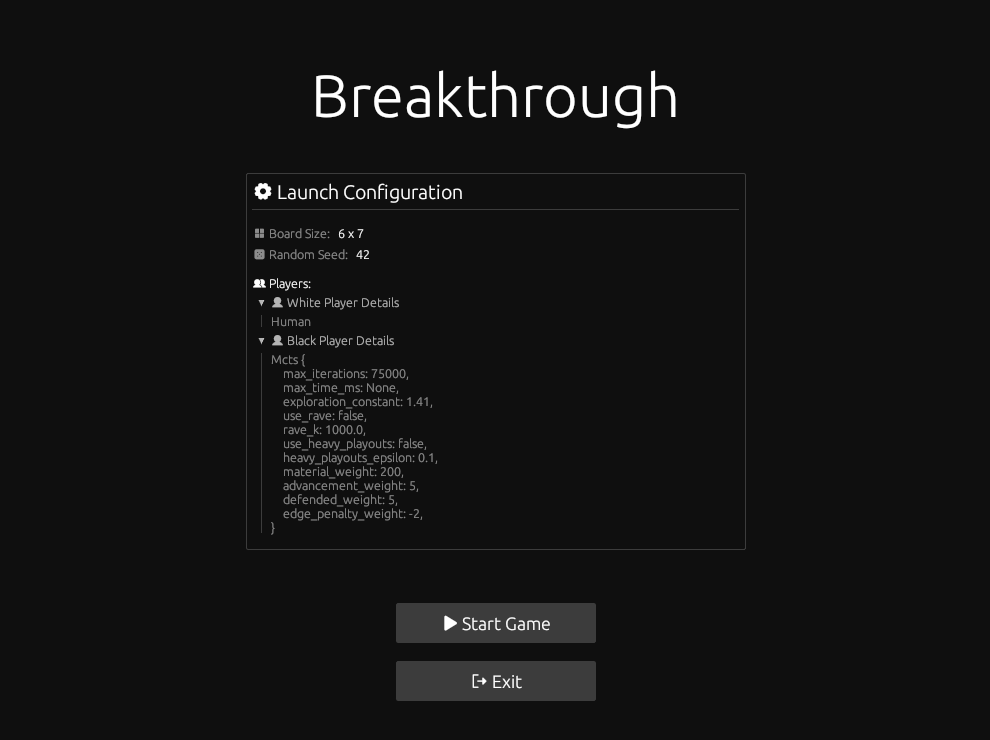
\includegraphics[width=\textwidth]{images/main_menu.png}
        \caption{Ekran startowy.}
        \label{fig:gui-main}
    \end{subfigure}
    \hfill
    \begin{subfigure}[b]{0.49\textwidth}
        \centering
        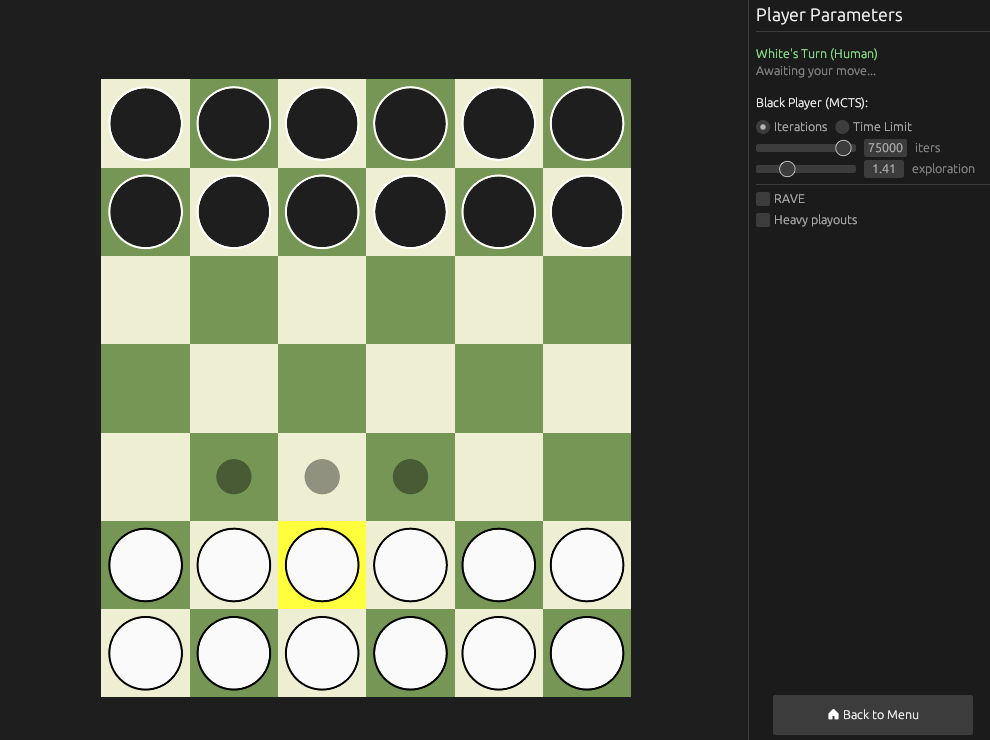
\includegraphics[width=\textwidth]{images/human_turn.png}
        \caption{Oczekiwanie na ruch gracza.}
        \label{fig:gui-human}
    \end{subfigure}

    \vspace{0.5cm}


    \begin{subfigure}[b]{0.49\textwidth}
        \centering
        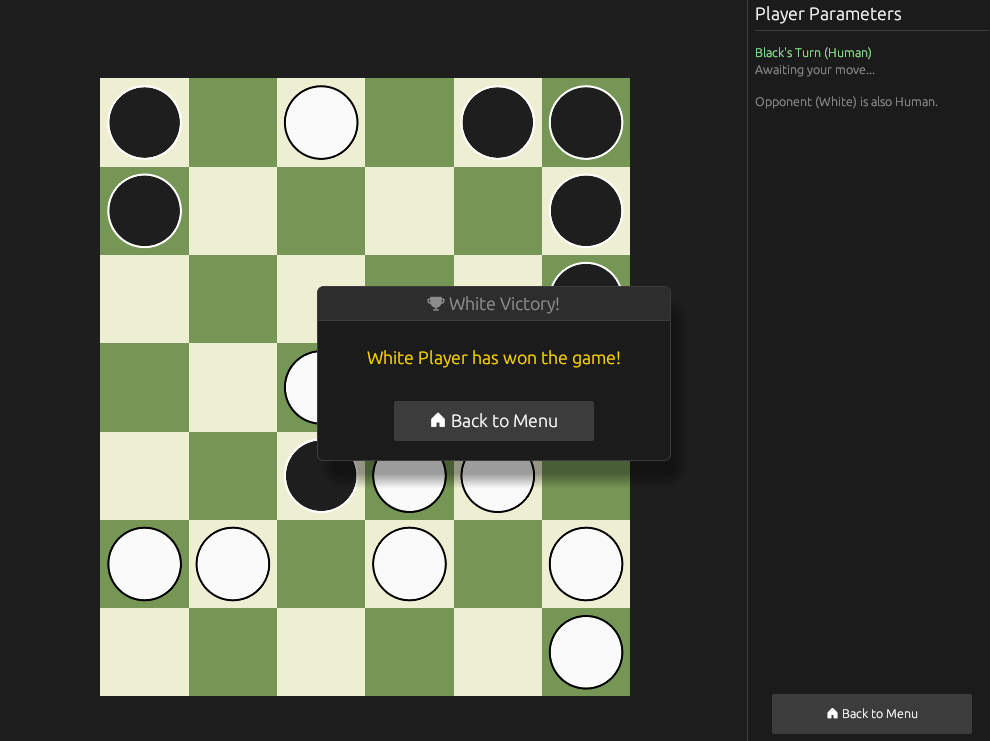
\includegraphics[width=\textwidth]{images/player_won.png}
        \caption{Ekran końcowy z ogłoszeniem zwycięzcy.}
        \label{fig:gui-won}
    \end{subfigure}
    \hfill
    \begin{subfigure}[b]{0.49\textwidth}
        \centering
        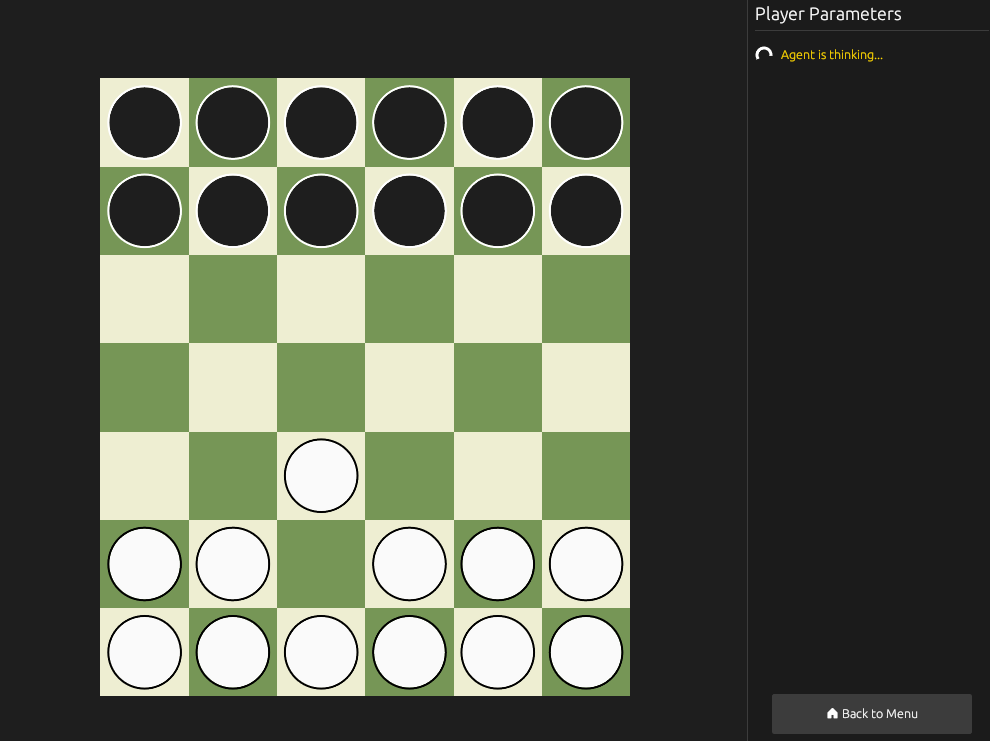
\includegraphics[width=\textwidth]{images/mcts_turn.png}
        \caption{Oczekiwanie na ruch agenta.}
        \label{fig:gui-mcts}
    \end{subfigure}

    \vspace{0.5cm}

    \begin{subfigure}[b]{0.49\textwidth}
        \centering
        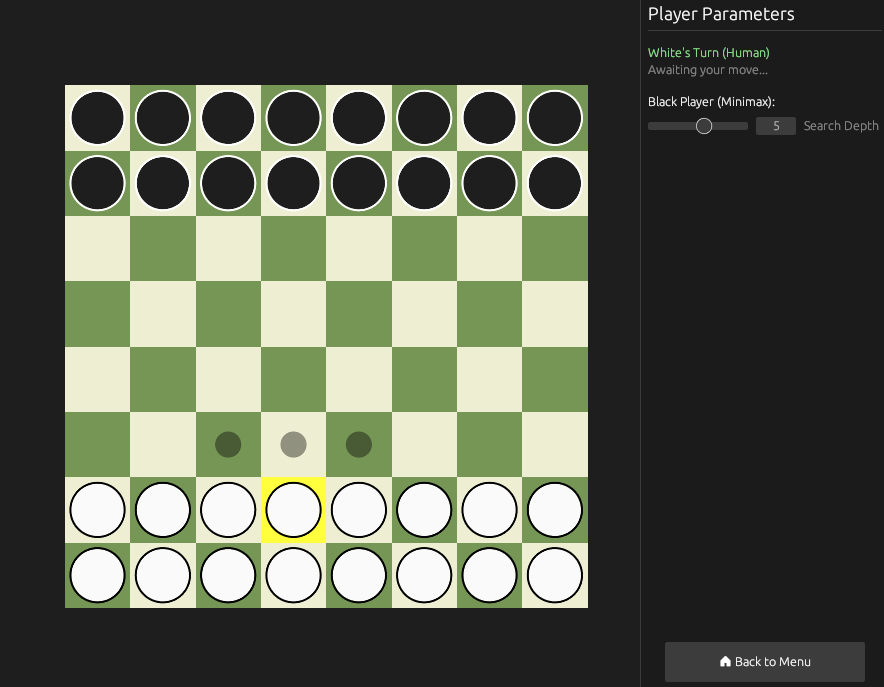
\includegraphics[width=\textwidth]{images/minimax_turn.png}
        \caption{Gra z agentem Minimax.}
        \label{fig:gui-minimax}
    \end{subfigure}

    \caption{Zrzuty ekranu interfejsu graficznego dla gry Breakthrough.}
    \label{fig:gui-overview}
\end{figure}

\newpage
\section{Weryfikacja hipotez badawczych}

\subsection{Hipoteza 1: Wpływ algorytmu RAVE}

\subsubsection{Metodologia i przebieg eksperymentu}

Pierwsza hipoteza badawcza dotyczyła bezpośredniego porównania klasycznego algorytmu MCTS z jego rozszerzeniem wykorzystującym heurystykę RAVE (ang. \textit{Rapid Action Value Estimation}). Celem eksperymentu było sprawdzenie, czy w warunkach stałego budżetu obliczeniowego, zdefiniowanego jako limit iteracji, wariant MCTS + RAVE osiągnie przewagę nad MCTS. Kryterium przyjęcia hipotezy było przekroczenie progu 55\% zwycięstw przez agenta MCTS + RAVE w bezpośrednim starciu z agentem MCTS.

W każdej rozgrywce obaj agenci korzystali z identycznego limitu iteracji równego 10~000. Na wstępie dostrojono hiperparametr $k$ algorytmu RAVE. Z testów wynikało, że wartość $k = 100$ dawała lepsze wyniki niż wartość domyślna $k = 1000$. Parametr $k$ kontroluje tempo zaniku wpływu statystyk AMAF zgodnie ze wzorem:

$$
\beta = \frac{k}{k + n}
$$

\noindent
gdzie $n$ oznacza liczbę odwiedzin rozpatrywanego węzła potomnego. Mniejsza wartość $k$ powoduje zatem szybsze przejście od wartości RAVE do klasycznych statystyk UCT.

Eksperyment przeprowadzono na czterech rozmiarach planszy: $6 \times 8$, $7 \times 7$, $8 \times 6$ oraz $8 \times 8$. Dla każdego rozmiaru planszy rozegrano 50 partii: 25 z agentem MCTS + RAVE jako graczem białym oraz 25 z agentem MCTS + RAVE jako graczem czarnym. Rotacja kolorów została zastosowana w celu ograniczenia wpływu przewagi pierwszego ruchu. Jak pokazują dalsze wyniki, kolor kontrolowanych pionów miał zauważalny wpływ na rezultaty. Łącznie w ramach weryfikacji hipotezy H1 rozegrano 200 partii.

\subsubsection{Analiza wyników}

Zestawienie współczynnika zwycięstw agenta MCTS + RAVE względem klasycznego MCTS przedstawiono na Rysunku~\ref{fig:h1-rave-winrate}. Pierwszy wykres agreguje wyniki według rozmiaru planszy, natomiast drugi dodatkowo rozdziela rezultaty ze względu na kolor kontrolowany przez agenta RAVE. Pozioma linia oznacza próg 55\% zwycięstw, wymagany do pozytywnej weryfikacji hipotezy.

\begin{figure}[H]
    \centering

    \begin{subfigure}[b]{0.49\textwidth}
        \centering
        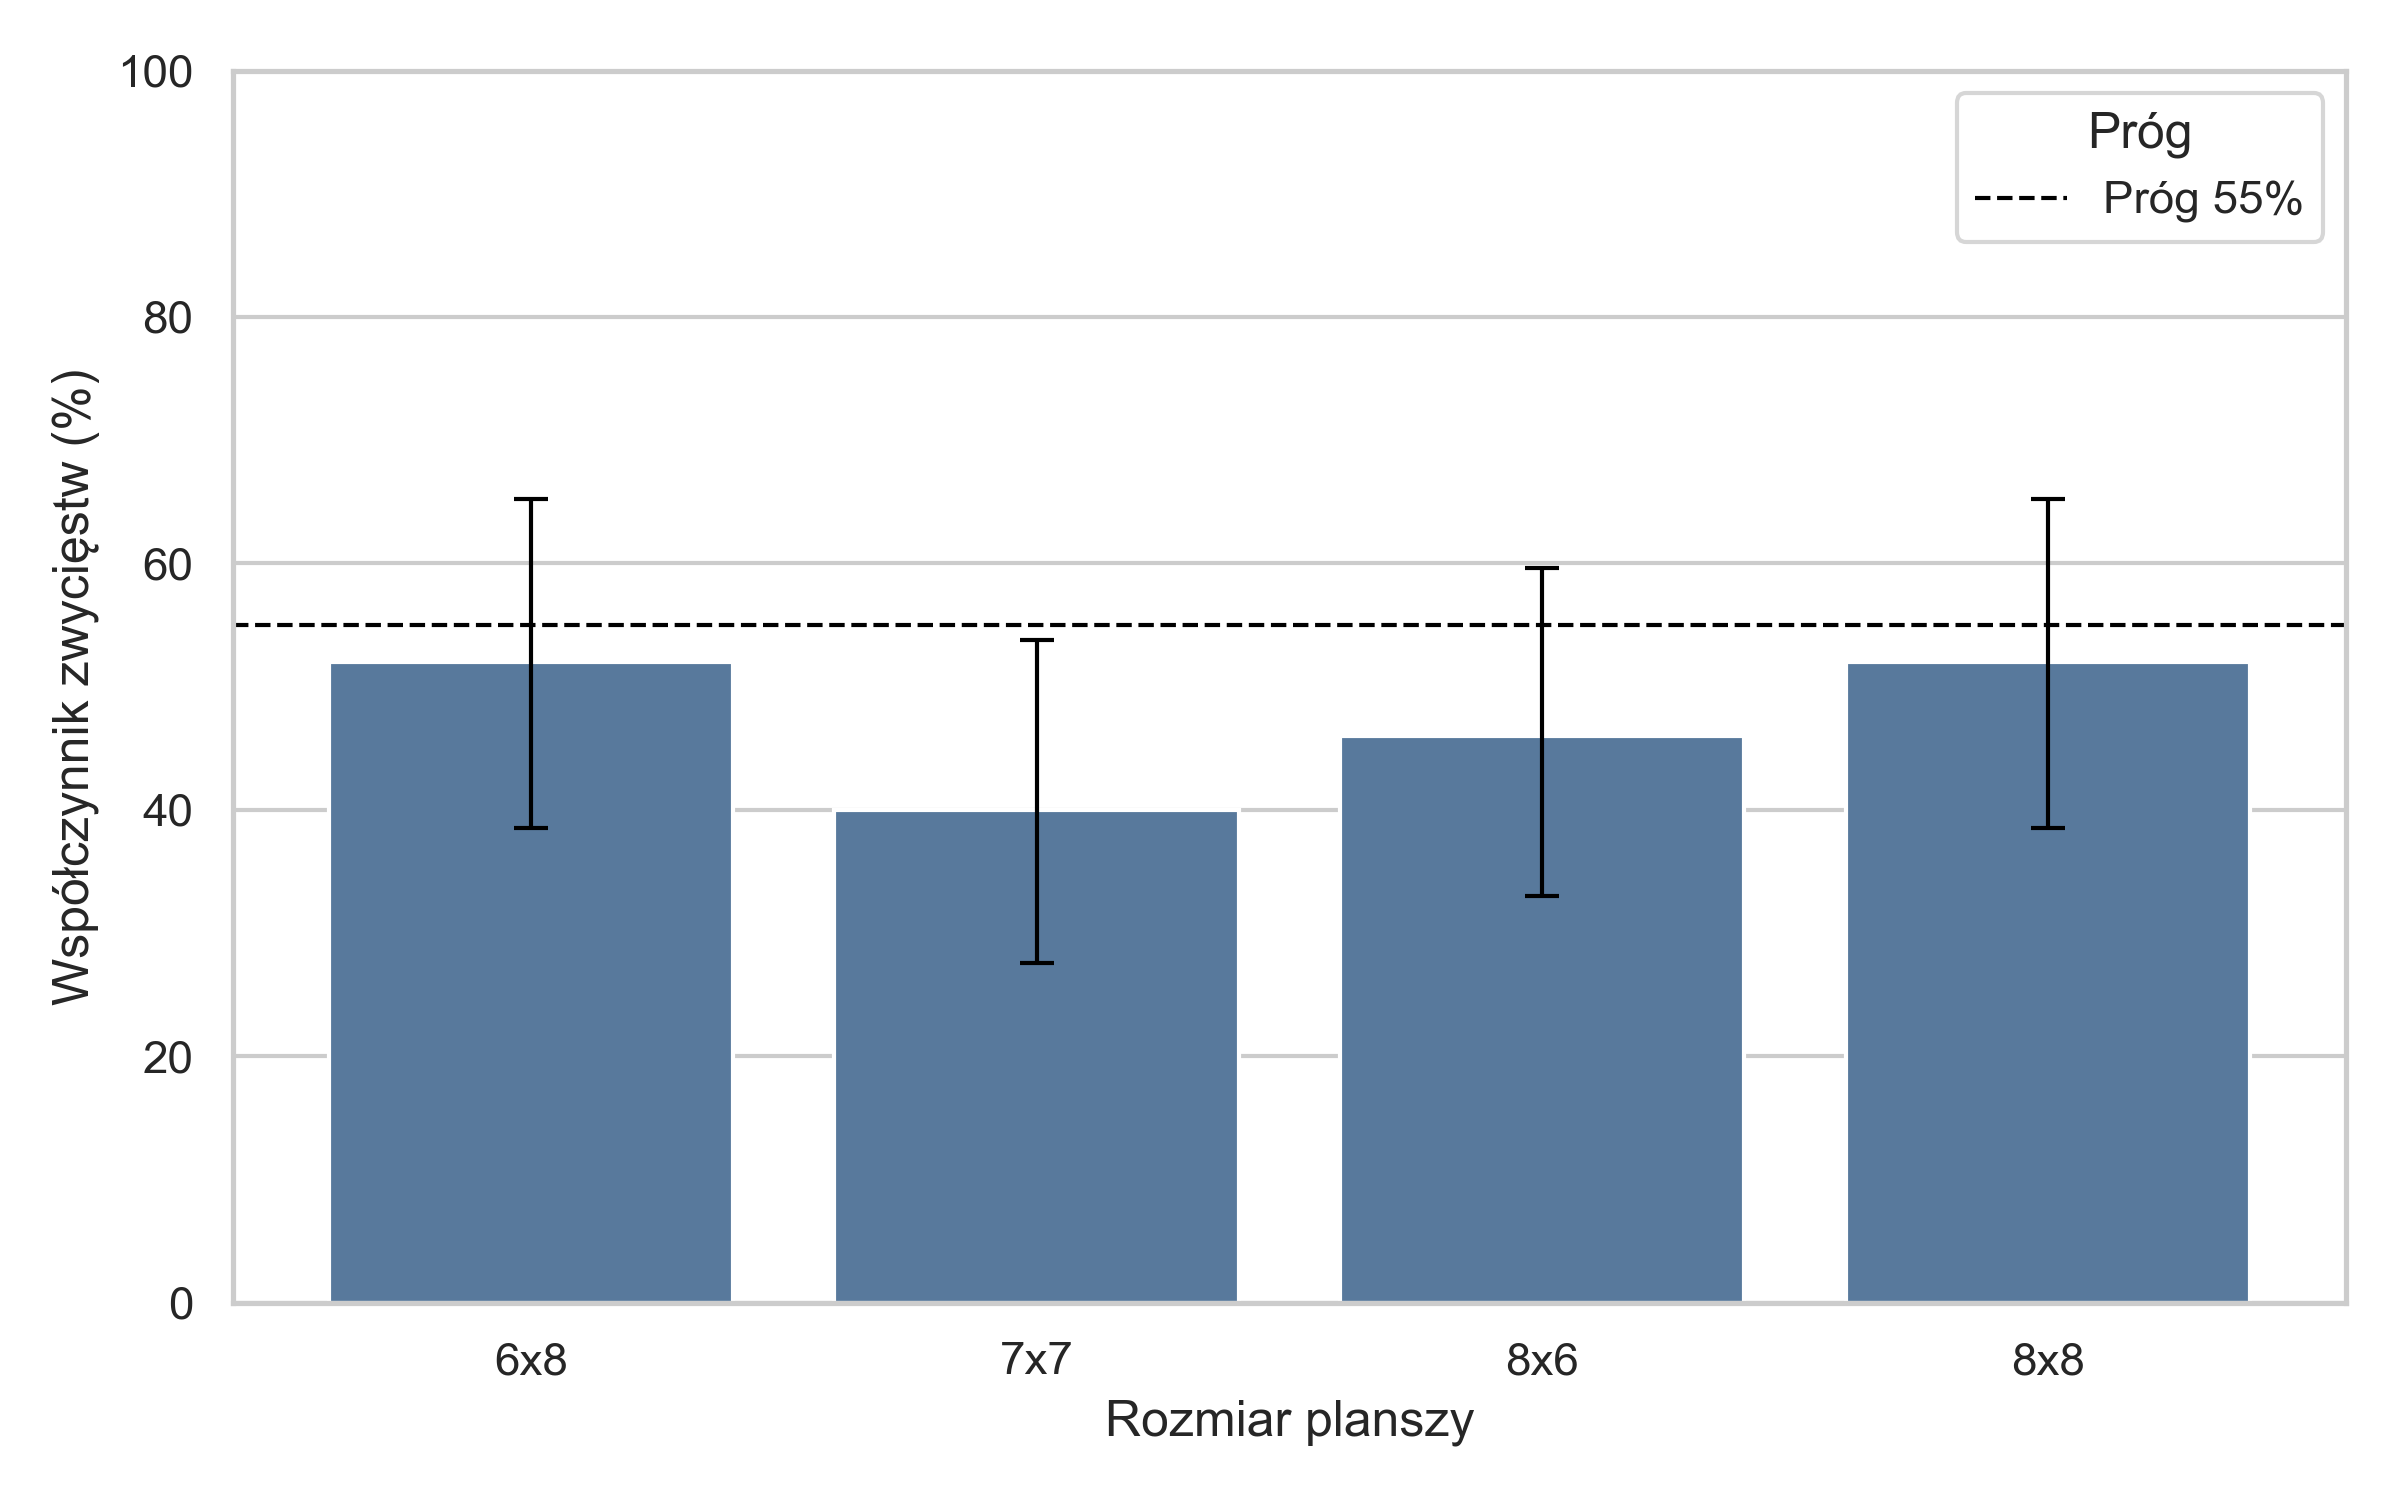
\includegraphics[width=\textwidth]{images/h1_rave_win_rate_by_board.png}
        \caption{Wyniki zagregowane według rozmiaru planszy}
        \label{fig:h1-rave-board}
    \end{subfigure}
    \hfill
    \begin{subfigure}[b]{0.49\textwidth}
        \centering
        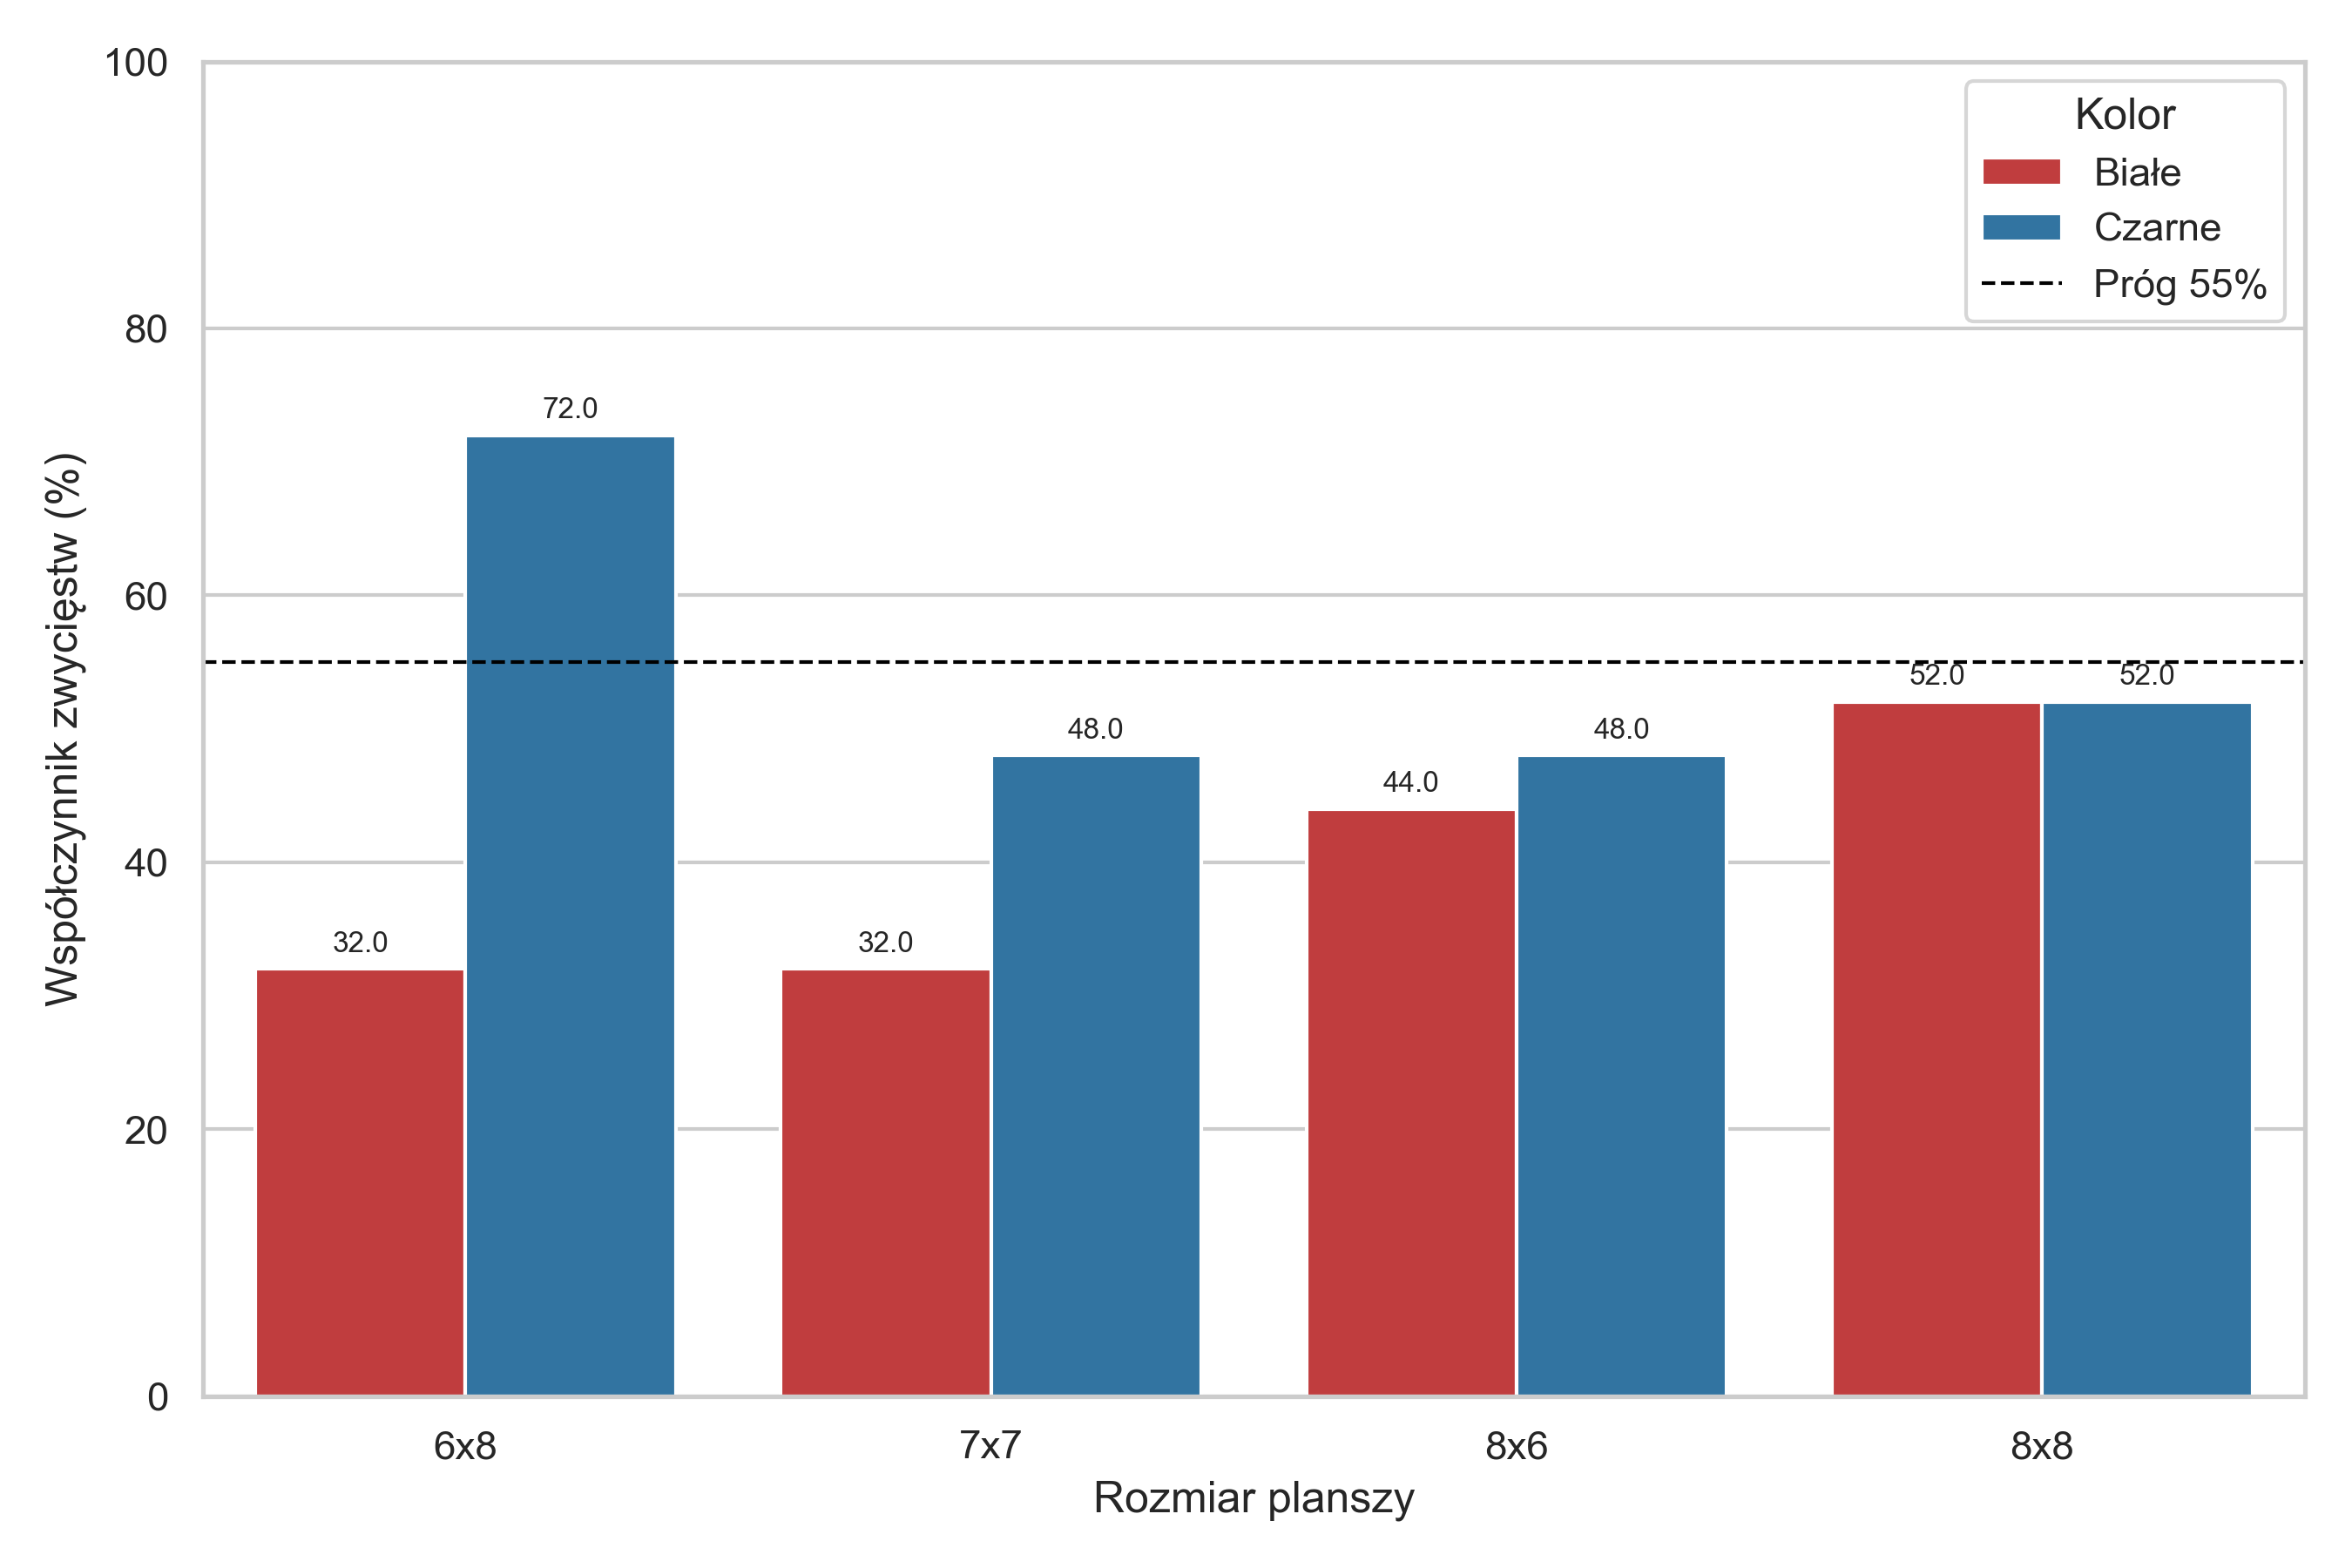
\includegraphics[width=\textwidth]{images/h1_rave_win_rate_by_board_and_color.png}
        \caption{Wyniki z podziałem na kolor agenta RAVE}
        \label{fig:h1-rave-board-color}
    \end{subfigure}

    \caption{Współczynnik zwycięstw agenta MCTS + RAVE w starciu z klasycznym MCTS przy limicie 10~000 iteracji na ruch.}
    \label{fig:h1-rave-winrate}
\end{figure}

\noindent
Wyniki liczbowe przedstawiono w Tabeli~\ref{tab:h1-summary}. W żadnym z badanych rozmiarów planszy średni wynik MCTS + RAVE nie przekroczył progu 55\%. Największą skuteczność agent uzyskiwał na planszach $6 \times 8$ oraz $8 \times 8$, gdzie wariant RAVE wygrał 52.0\% partii. Najsłabszy rezultat odnotowano na planszy $7 \times 7$, gdzie współczynnik zwycięstw wyniósł 40.0\%.

\begin{table}[H]
    \centering
    \caption{Wyniki eksperymentu H1: MCTS + RAVE przeciwko klasycznemu MCTS.}
    \label{tab:h1-summary}
    \renewcommand{\arraystretch}{1.2}
    \begin{tabular}{|c|c|c|c|}
        \hline
        \textbf{Rozmiar planszy} & \textbf{Zwycięstwa RAVE} & \textbf{Skuteczność} & \textbf{Średnia długość partii} \\
        \hline
        $6 \times 8$ & 26/50 & 52.0\% & 46.7 \\
        $7 \times 7$ & 20/50 & 40.0\% & 43.5 \\
        $8 \times 6$ & 23/50 & 46.0\% & 42.1 \\
        $8 \times 8$ & 26/50 & 52.0\% & 54.4 \\
        \hline
        \textbf{Łącznie} & \textbf{95/200} & \textbf{47.5\%} & \textbf{46.7} \\
        \hline
    \end{tabular}
\end{table}

\noindent
Sumaryczny wynik MCTS + RAVE wyniósł 95 zwycięstw w 200 partiach, co odpowiada skuteczności 47.5\%. Przedział ufności Wilsona na poziomie 95\% wynosił $[40.7\%, 54.4\%]$, a więc nawet jego górna granica pozostaje poniżej progu 55\%.

Dodatkowych wniosków dostarcza analiza rozkładu długości partii, przedstawiona na Rysunku~\ref{fig:h1-game-length}.

\begin{figure}[H]
    \centering
    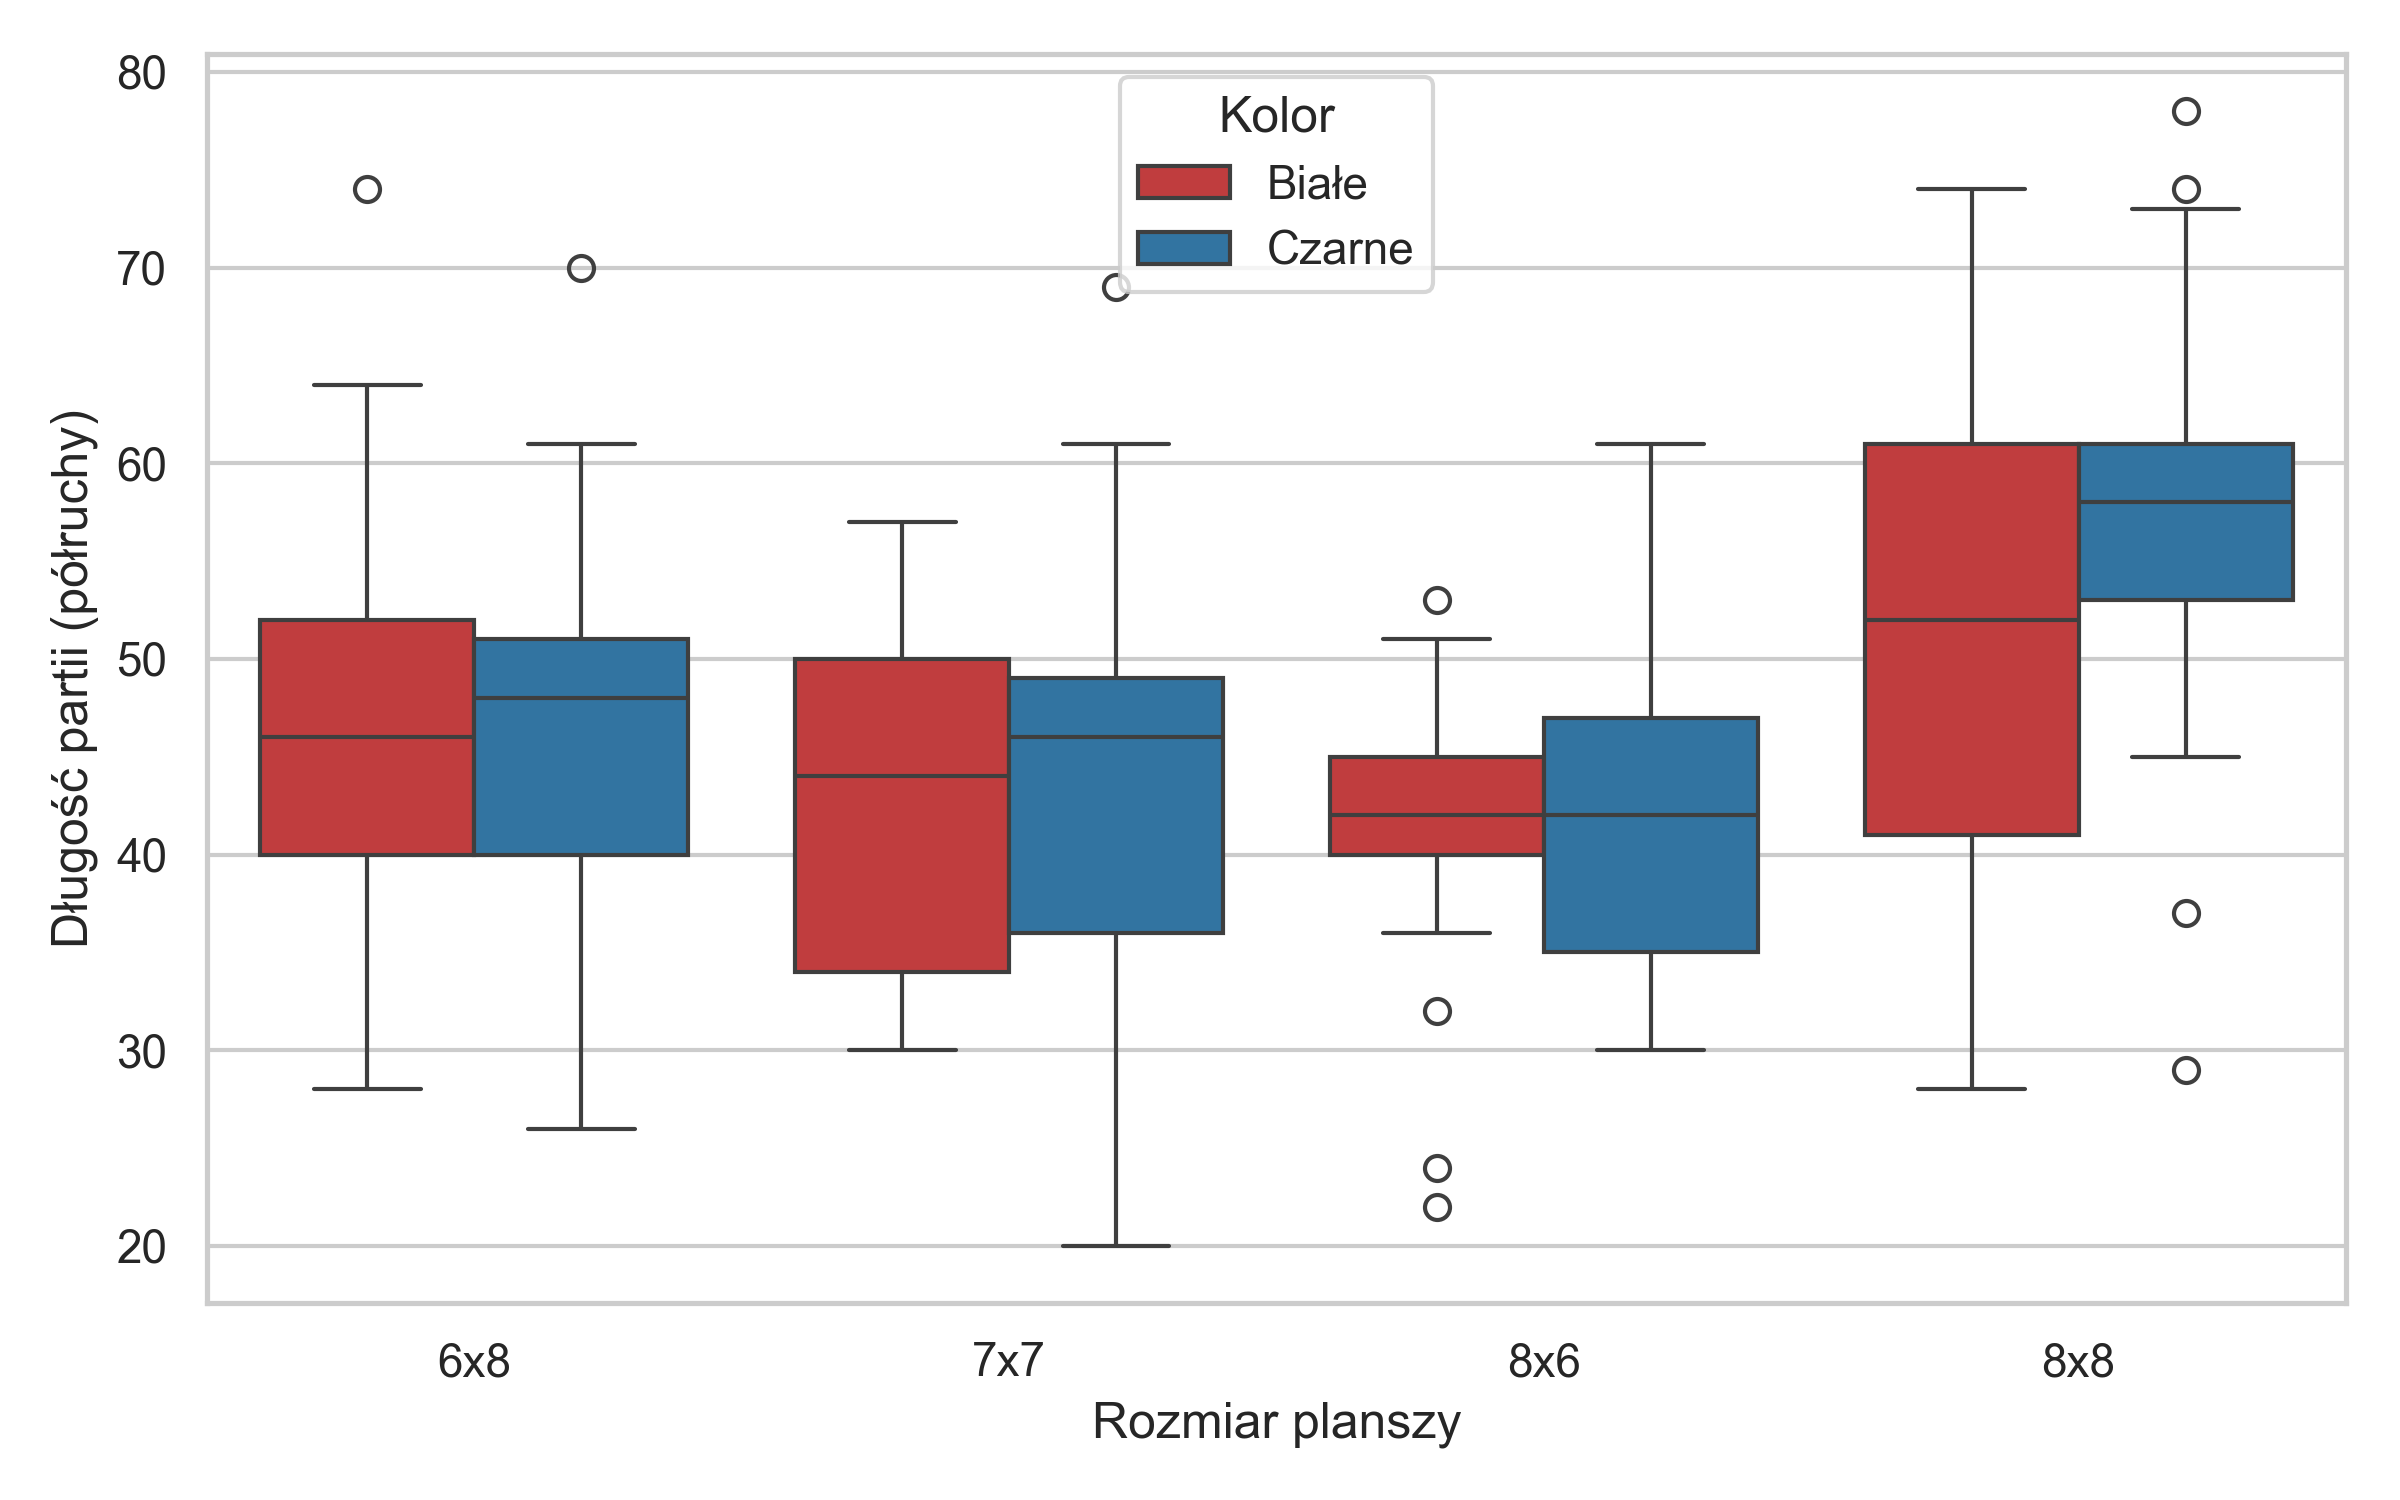
\includegraphics[width=0.8\textwidth]{images/h1_game_length_by_board_and_color.png}
    \caption{Rozkład długości partii (w półruchach) w eksperymencie H1 z podziałem na rozmiar planszy i kolor.}
    \label{fig:h1-game-length}
\end{figure}

\noindent
Rozkład liczby rozegranych półruchów wykazuje silną zależność od fizycznych proporcji planszy. Najkrótsze partie odnotowano na planszy $8 \times 6$ (średnio 42.1 półruchów). Wynika to z faktu, że odległość do końcowej linii przeciwnika wynosi tylko 6 rzędów, co naturalnie skraca rozgrywkę. Z kolei na planszy $8 \times 8$, wymagającej pokonania najdłuższego dystansu przy zachowaniu dużej szerokości frontu, gry były zauważalnie dłuższe (średnio 54.4 półruchów), a rozrzut wyników był największy. Zaskakującą obserwacją jest to, że w trzech z czterech rozmiarów planszy agent RAVE, grając po stronie czarnej, wykonywał średnio więcej ruchów niż grając po stronie białej. Może być to związane ze zwiększoną liczbą zwycięstw odnoszonych po stronie czarnej, choć na pierwszy rzut oka jest to sprzeczne z intuicją: gracz biały, rozpoczynając partię, ma możliwość wykonania jednego ruchu więcej od przeciwnika. Poza tą obserwacją dla badanego wariantu nie zaobserwowano jednoznacznych różnic w długości rozgrywki pomiędzy dwoma kolorami kontrolowanych pionów.

\subsubsection{Wnioski końcowe}

\textbf{Hipoteza H1 zostaje odrzucona}. Dla limitu 10~000 iteracji na ruch agent MCTS + RAVE, nawet po dobraniu korzystniejszego parametru $k = 100$, nie osiągnął wymaganego progu 55\% zwycięstw w bezpośrednim starciu z bazowym MCTS. Wynik sugeruje, że w badanej implementacji i dla przyjętych rozmiarów planszy informacja AMAF nie poprawia stabilnie jakości decyzji względem klasycznego MCTS. Możliwym wyjaśnieniem jest fakt, że w grze Breakthrough kolejność ruchów oraz tempo dojścia do linii końcowej mają duże znaczenie taktyczne. Dodatkowo przypadkowe ruchy wykonywane w fazie \textit{playout} mogą nie nieść wystarczająco użytecznej informacji AMAF, przez co założenie RAVE o użyteczności ruchu niezależnie od momentu jego wykonania okazuje się w tym środowisku zbyt silne i może prowadzić do przeszukiwania nieoptymalnych gałęzi drzewa gry.

\newpage
\subsection{Hipoteza 2: Wpływ algorytmu Heavy Playouts}

\subsubsection{Metodologia i przebieg eksperymentu}

Druga hipoteza badawcza dotyczyła wpływu ukierunkowania fazy \textit{playout} zgodnie z przyjętą funkcją heurystyczną, na jakość decyzji podejmowanych przez agenta MCTS. W odróżnieniu od eksperymentu H1, w tej serii pomiarowej nie narzucono stałej liczby iteracji. Wynika to z faktu, że pojedyncza iteracja agenta Heavy Playouts jest znacznie wolniejsza, ponieważ symulacja rozgrywki od liścia drzewa wymaga dodatkowej oceny pozycji, a nie jedynie wyboru losowego legalnego ruchu. Z tego powodu zastosowano limit czasowy, który lepiej odpowiada realistycznym ograniczeniom decyzyjnym. Celem było sprawdzenie, czy agent MCTS + Heavy Playouts osiąga współczynnik zwycięstw powyżej 55\% w bezpośrednim starciu z bazowym MCTS.

Limit czasu wynosił 250 milisekund, co pozwoliło utrzymać akceptowalny czas całego eksperymentu przy zachowaniu porównywalnych warunków dla obu agentów. Obaj gracze korzystali z tego samego limitu czasowego. Dodatkowo agent MCTS + Heavy Playouts w fazie symulacji wykorzystywał strategię $\epsilon$-greedy z parametrem $\epsilon = 0.1$, dzięki czemu z prawdopodobieństwem 10\% wykonywał losowy legalny ruch, a w pozostałych przypadkach kierował się oceną heurystyczną.

Podobnie jak w przypadku H1, eksperyment przeprowadzono na planszach $6 \times 8$, $7 \times 7$, $8 \times 6$ oraz $8 \times 8$. Dla każdego rozmiaru planszy rozegrano 40 partii: 20 z agentem MCTS + Heavy Playouts jako graczem białym oraz 20 z tym samym agentem jako graczem czarnym. Łącznie w celu weryfikacji hipotezy H2 rozegrano 160 partii.

\subsubsection{Analiza wyników}

Wyniki eksperymentu przedstawiono na Rysunku~\ref{fig:h2-heavy-winrate}. Są one przeciwne do obserwacji uzyskanych dla hipotezy H1. Wariant wykorzystujący Heavy Playouts zdecydowanie przekroczył próg 55\% dla każdego badanego rozmiaru planszy. Najniższą skuteczność osiągnął na planszach $7 \times 7$ oraz $8 \times 8$, gdzie współczynnik zwycięstw wyniósł 87.5\%. Najlepszy rezultat uzyskano na planszy $6 \times 8$, gdzie agent wygrał 38 z 40 rozgrywek (95.0\%). Co istotne, wyraźna przewaga utrzymała się zarówno przy agregacji wyników, jak i przy rozbiciu na kolor kontrolowany przez agenta testowego. Dla każdego rozmiaru planszy agent MCTS + Heavy Playouts osiągał wyniki co najmniej tak dobre po stronie czarnej jak po stronie białej. Największą dysproporcję zaobserwowano dla planszy $8 \times 8$, gdzie współczynnik zwycięstw wyniósł 80\% dla białych oraz 95\% dla czarnych. Wynik 95\% pojawił się również dla czarnych na planszy $8 \times 6$ oraz dla obu kolorów na planszy $6 \times 8$.

\begin{figure}[H]
    \centering

    \begin{subfigure}[b]{0.49\textwidth}
        \centering
        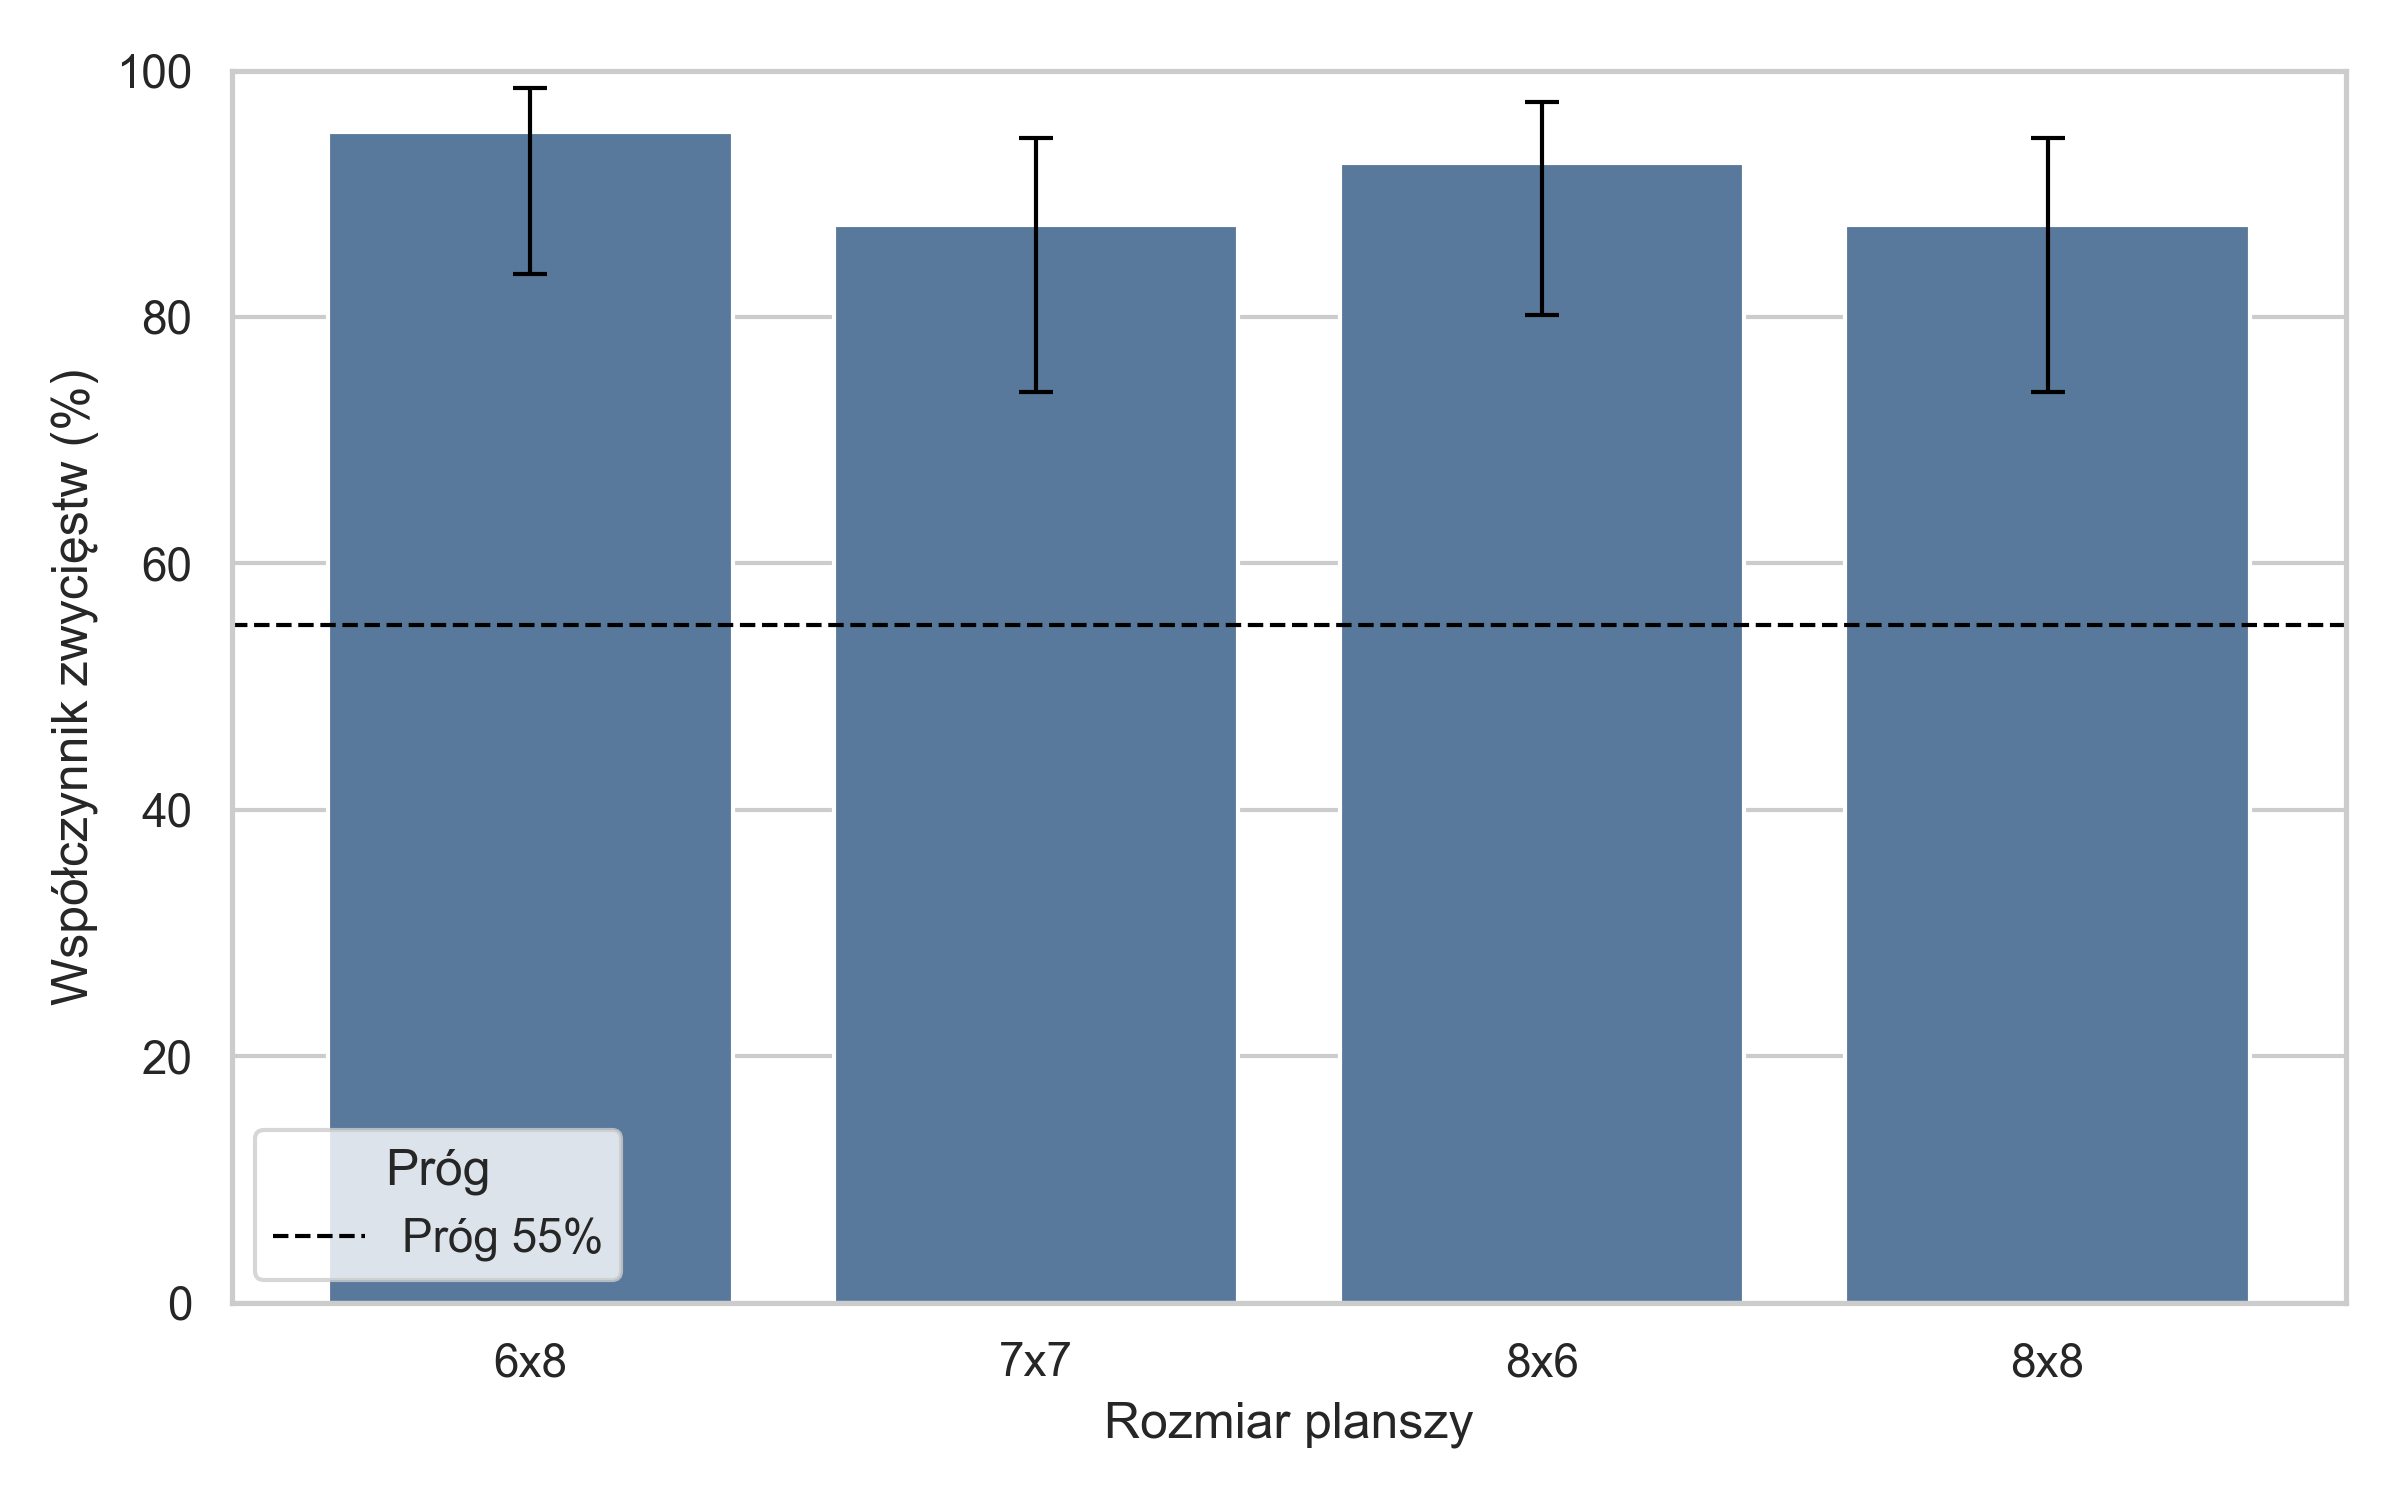
\includegraphics[width=\textwidth]{images/h2_heavyplayouts_win_rate_by_board.png}
        \caption{Wyniki zagregowane według rozmiaru planszy}
        \label{fig:h2-heavy-board}
    \end{subfigure}
    \hfill
    \begin{subfigure}[b]{0.49\textwidth}
        \centering
        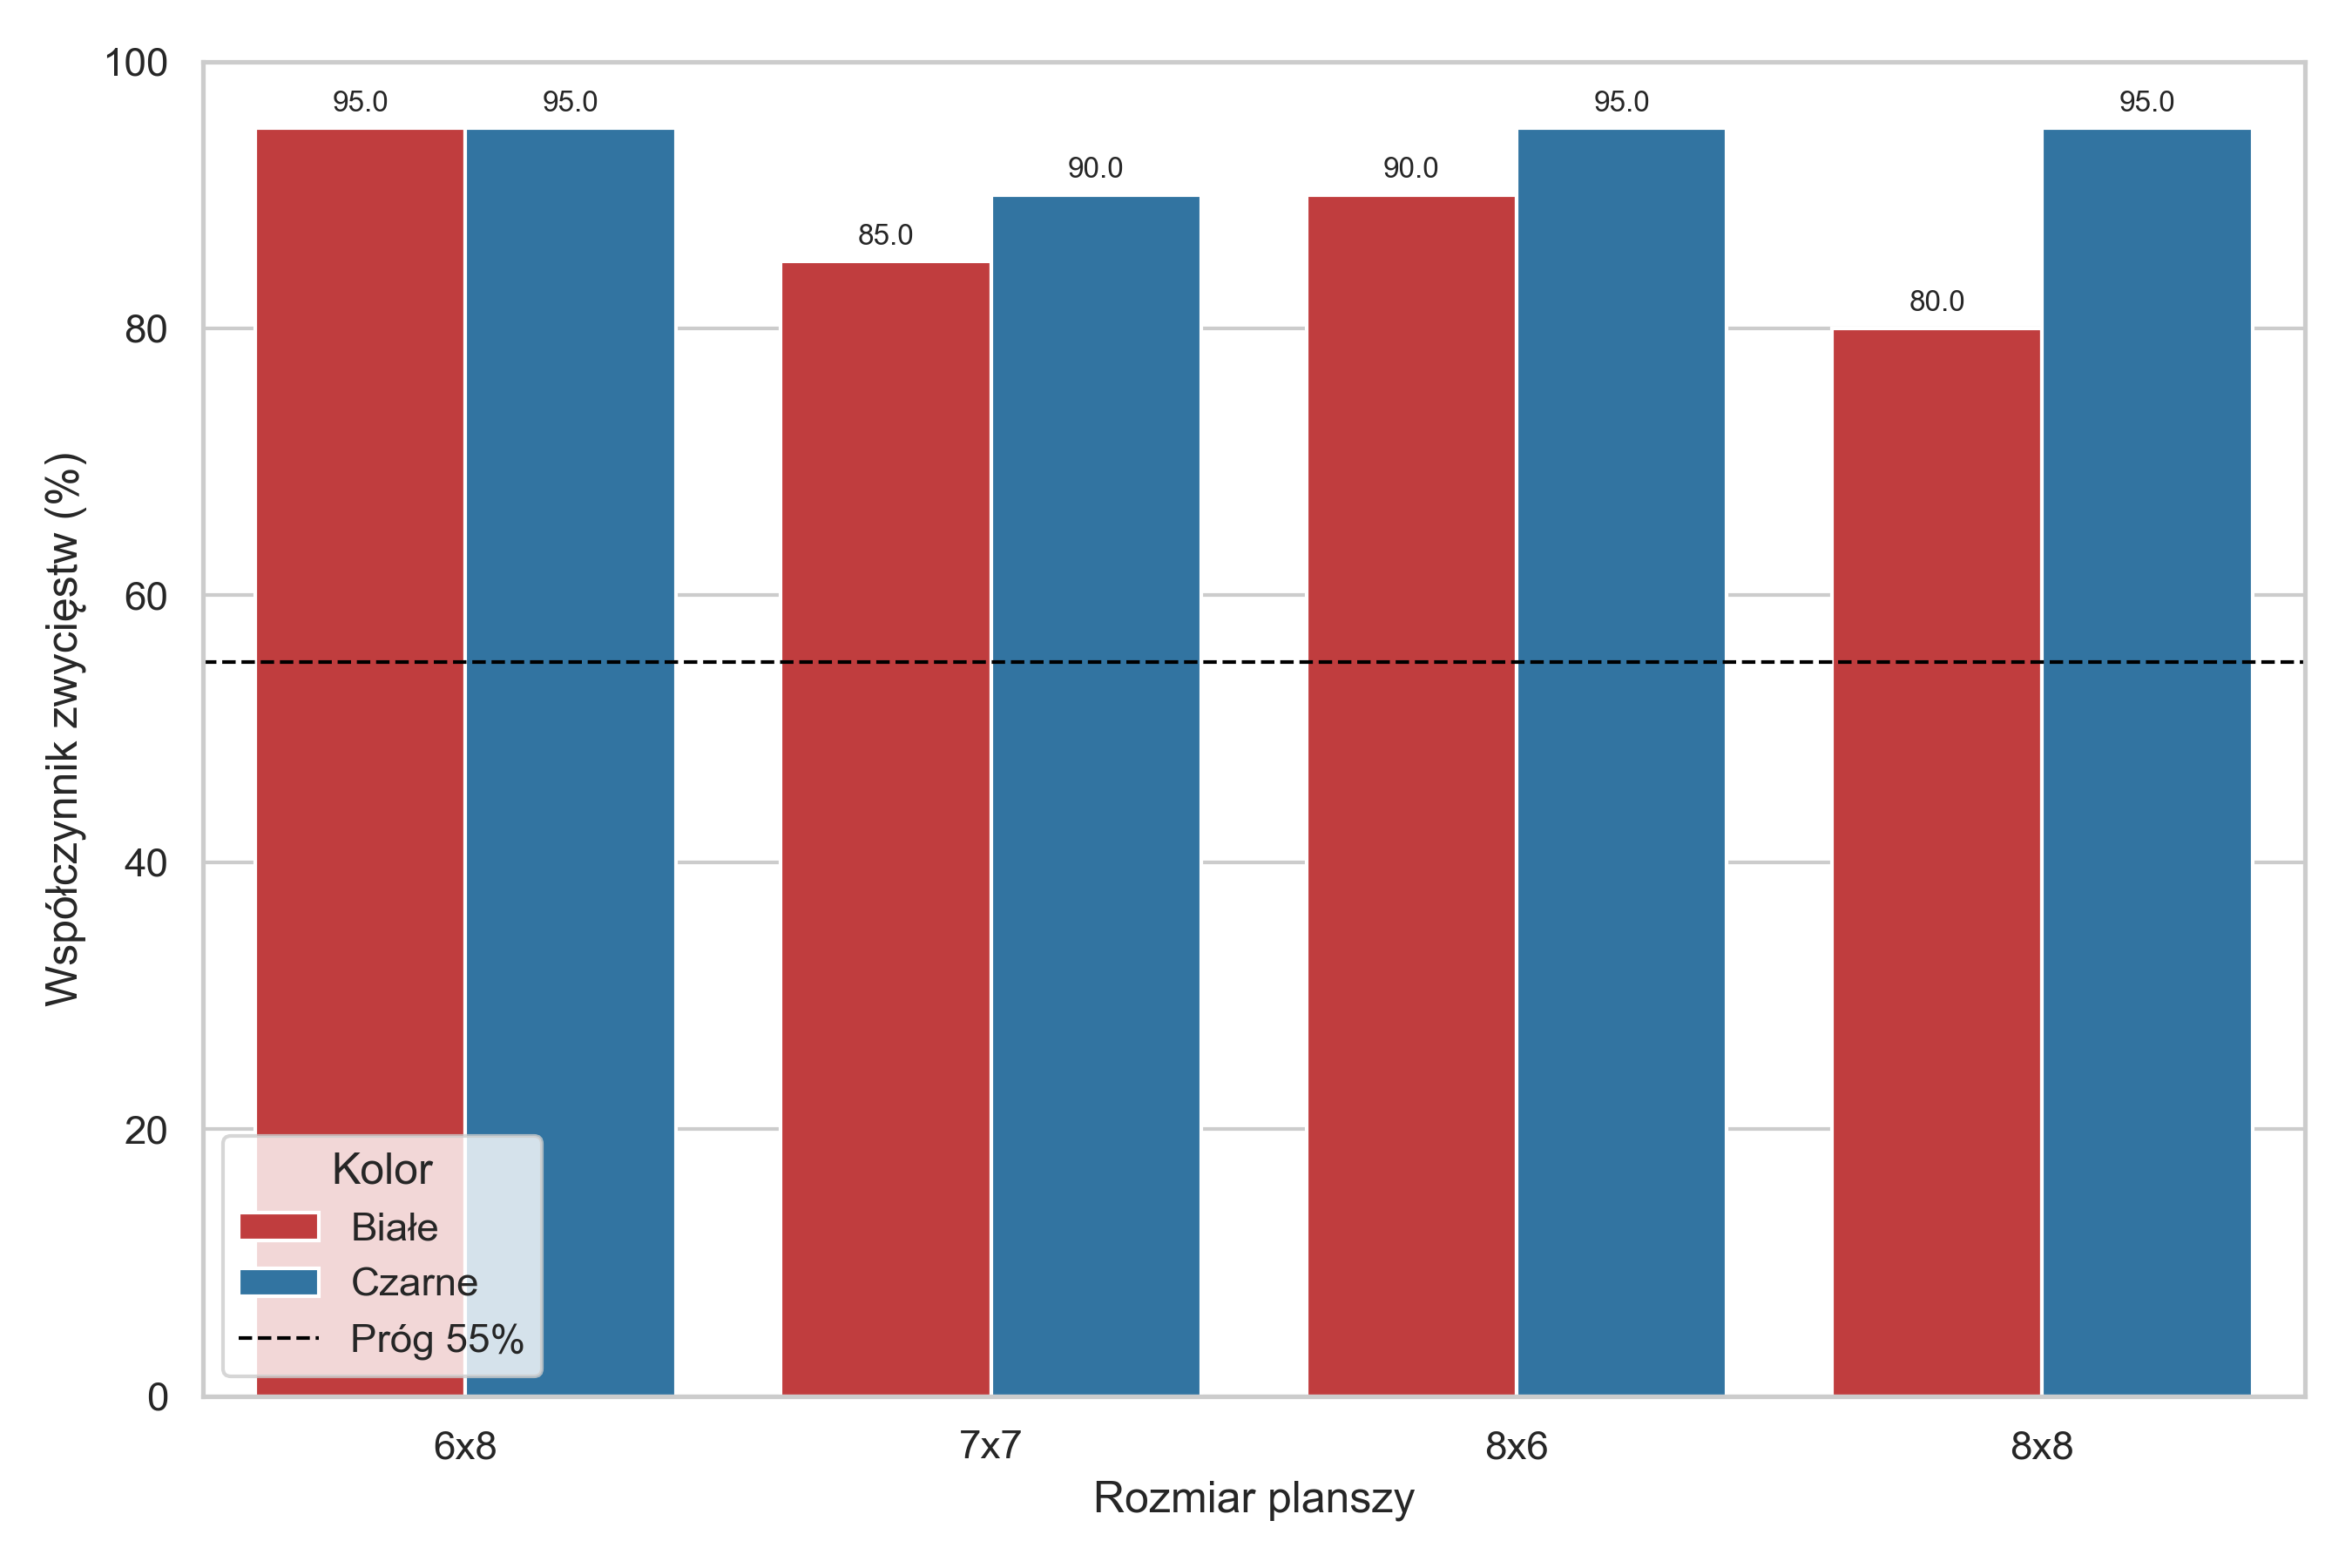
\includegraphics[width=\textwidth]{images/h2_heavyplayouts_win_rate_by_board_and_color.png}
        \caption{Wyniki z podziałem na kolor agenta}
        \label{fig:h2-heavy-board-color}
    \end{subfigure}

    \caption{Współczynnik zwycięstw agenta MCTS + Heavy Playouts w starciu z klasycznym MCTS przy limicie 250 ms na ruch.}
    \label{fig:h2-heavy-winrate}
\end{figure}

\noindent
Szczegółowe wyniki liczbowe oraz analizę obciążenia obliczeniowego przedstawiono w Tabeli~\ref{tab:h2-summary}.

\begin{table}[H]
    \centering
    \caption{Wyniki eksperymentu H2: MCTS + Heavy Playouts przeciwko klasycznemu MCTS.}
    \label{tab:h2-summary}
    \renewcommand{\arraystretch}{1.2}
    \begin{tabular}{|c|c|c|c|c|}
        \hline
        \textbf{Plansza} & \textbf{Zwycięstwa HP} & \textbf{Skuteczność} & \textbf{Śr. dł. partii} & \textbf{Śr. iteracje (HP / MCTS)} \\
        \hline
        $6 \times 8$ & 38/40 & 95.0\% & 53.4 & 1.19M / 3.67M \\
        $7 \times 7$ & 35/40 & 87.5\% & 47.8 & 0.91M / 3.37M \\
        $8 \times 6$ & 37/40 & 92.5\% & 38.1 & 0.90M / 2.86M \\
        $8 \times 8$ & 35/40 & 87.5\% & 61.0 & 0.60M / 2.82M \\
        \hline
        \textbf{Łącznie} & \textbf{145/160} & \textbf{90.6\%} & \textbf{50.1} & \textbf{--} \\
        \hline
    \end{tabular}
\end{table}

\noindent
Sumarycznie agent MCTS + Heavy Playouts wygrał 145 ze 160 partii, co daje skuteczność 90.6\%. Przedział ufności Wilsona na poziomie 95\% wynosił $[85.1\%, 94.2\%]$. Jest to przedział estymujący prawdopodobny zakres rzeczywistego współczynnika zwycięstw na podstawie skończonej próby 160 partii. Zastosowanie przedziału Wilsona jest korzystne dla danych procentowych, ponieważ daje stabilniejszą ocenę niepewności niż proste przybliżenie normalne, szczególnie gdy wynik znajduje się blisko 0\% lub 100\%. W tym przypadku cały przedział leży znacznie powyżej progu 55\%, co wzmacnia wniosek o pozytywnej weryfikacji hipotezy.

Kluczową obserwacją w tym eksperymencie jest duża dysproporcja w liczbie iteracji wykonywanych przez oba algorytmy w tym samym oknie czasowym (250 ms). Jak wcześniej wspomniano, wprowadzenie heurystyki do fazy \textit{playout} jest kosztowne obliczeniowo. W efekcie algorytm Heavy Playouts wykonywał średnio od około 3 do 4.7 razy mniej iteracji niż klasyczny wariant MCTS. Dla plansz $7 \times 7$ oraz $8 \times 8$ różnica ta była najwyższa (odpowiednio około 3.7 oraz 4.7) i korelowała z nieco niższą skutecznością agenta. Dla plansz $6 \times 8$ i $8 \times 6$ relacja wynosiła około 3.1 iteracji klasycznego MCTS na jedną iterację Heavy Playouts.

\begin{figure}[H]
    \centering

    \begin{subfigure}[b]{0.49\textwidth}
        \centering
        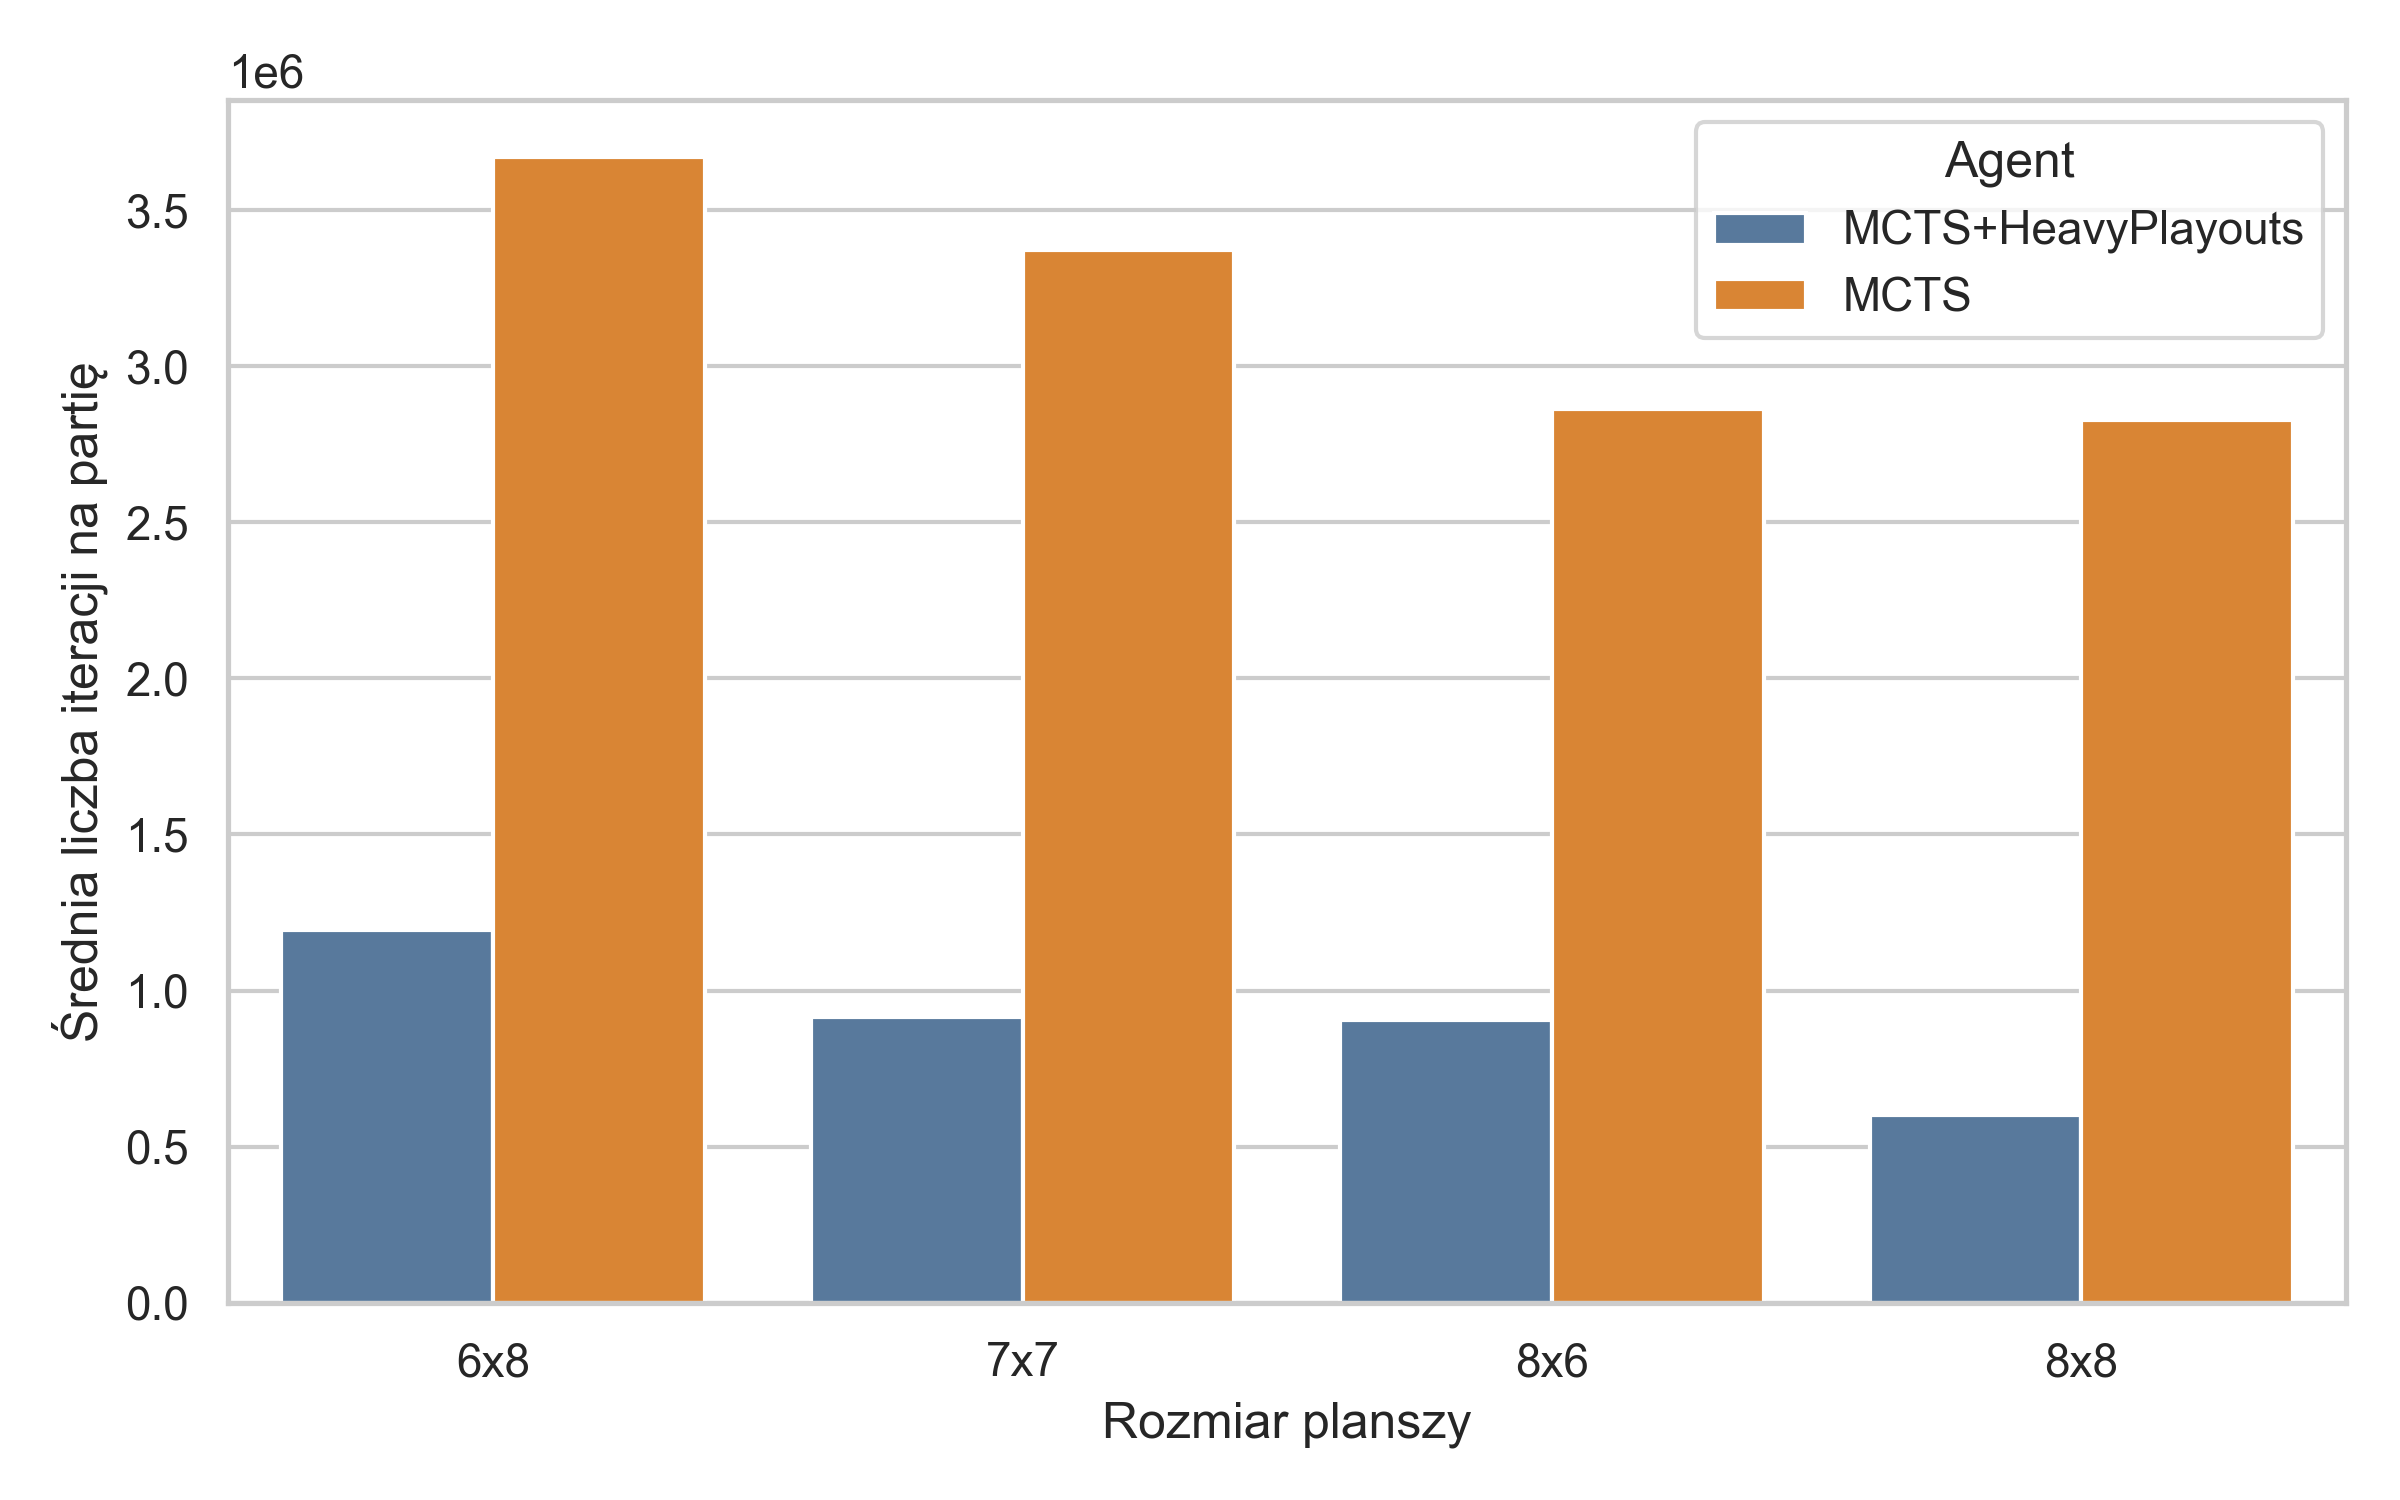
\includegraphics[width=\textwidth]{images/h2_iterations_by_board.png}
        \caption{Średnia liczba iteracji}
        \label{fig:h2-iterations}
    \end{subfigure}
    \hfill
    \begin{subfigure}[b]{0.49\textwidth}
        \centering
        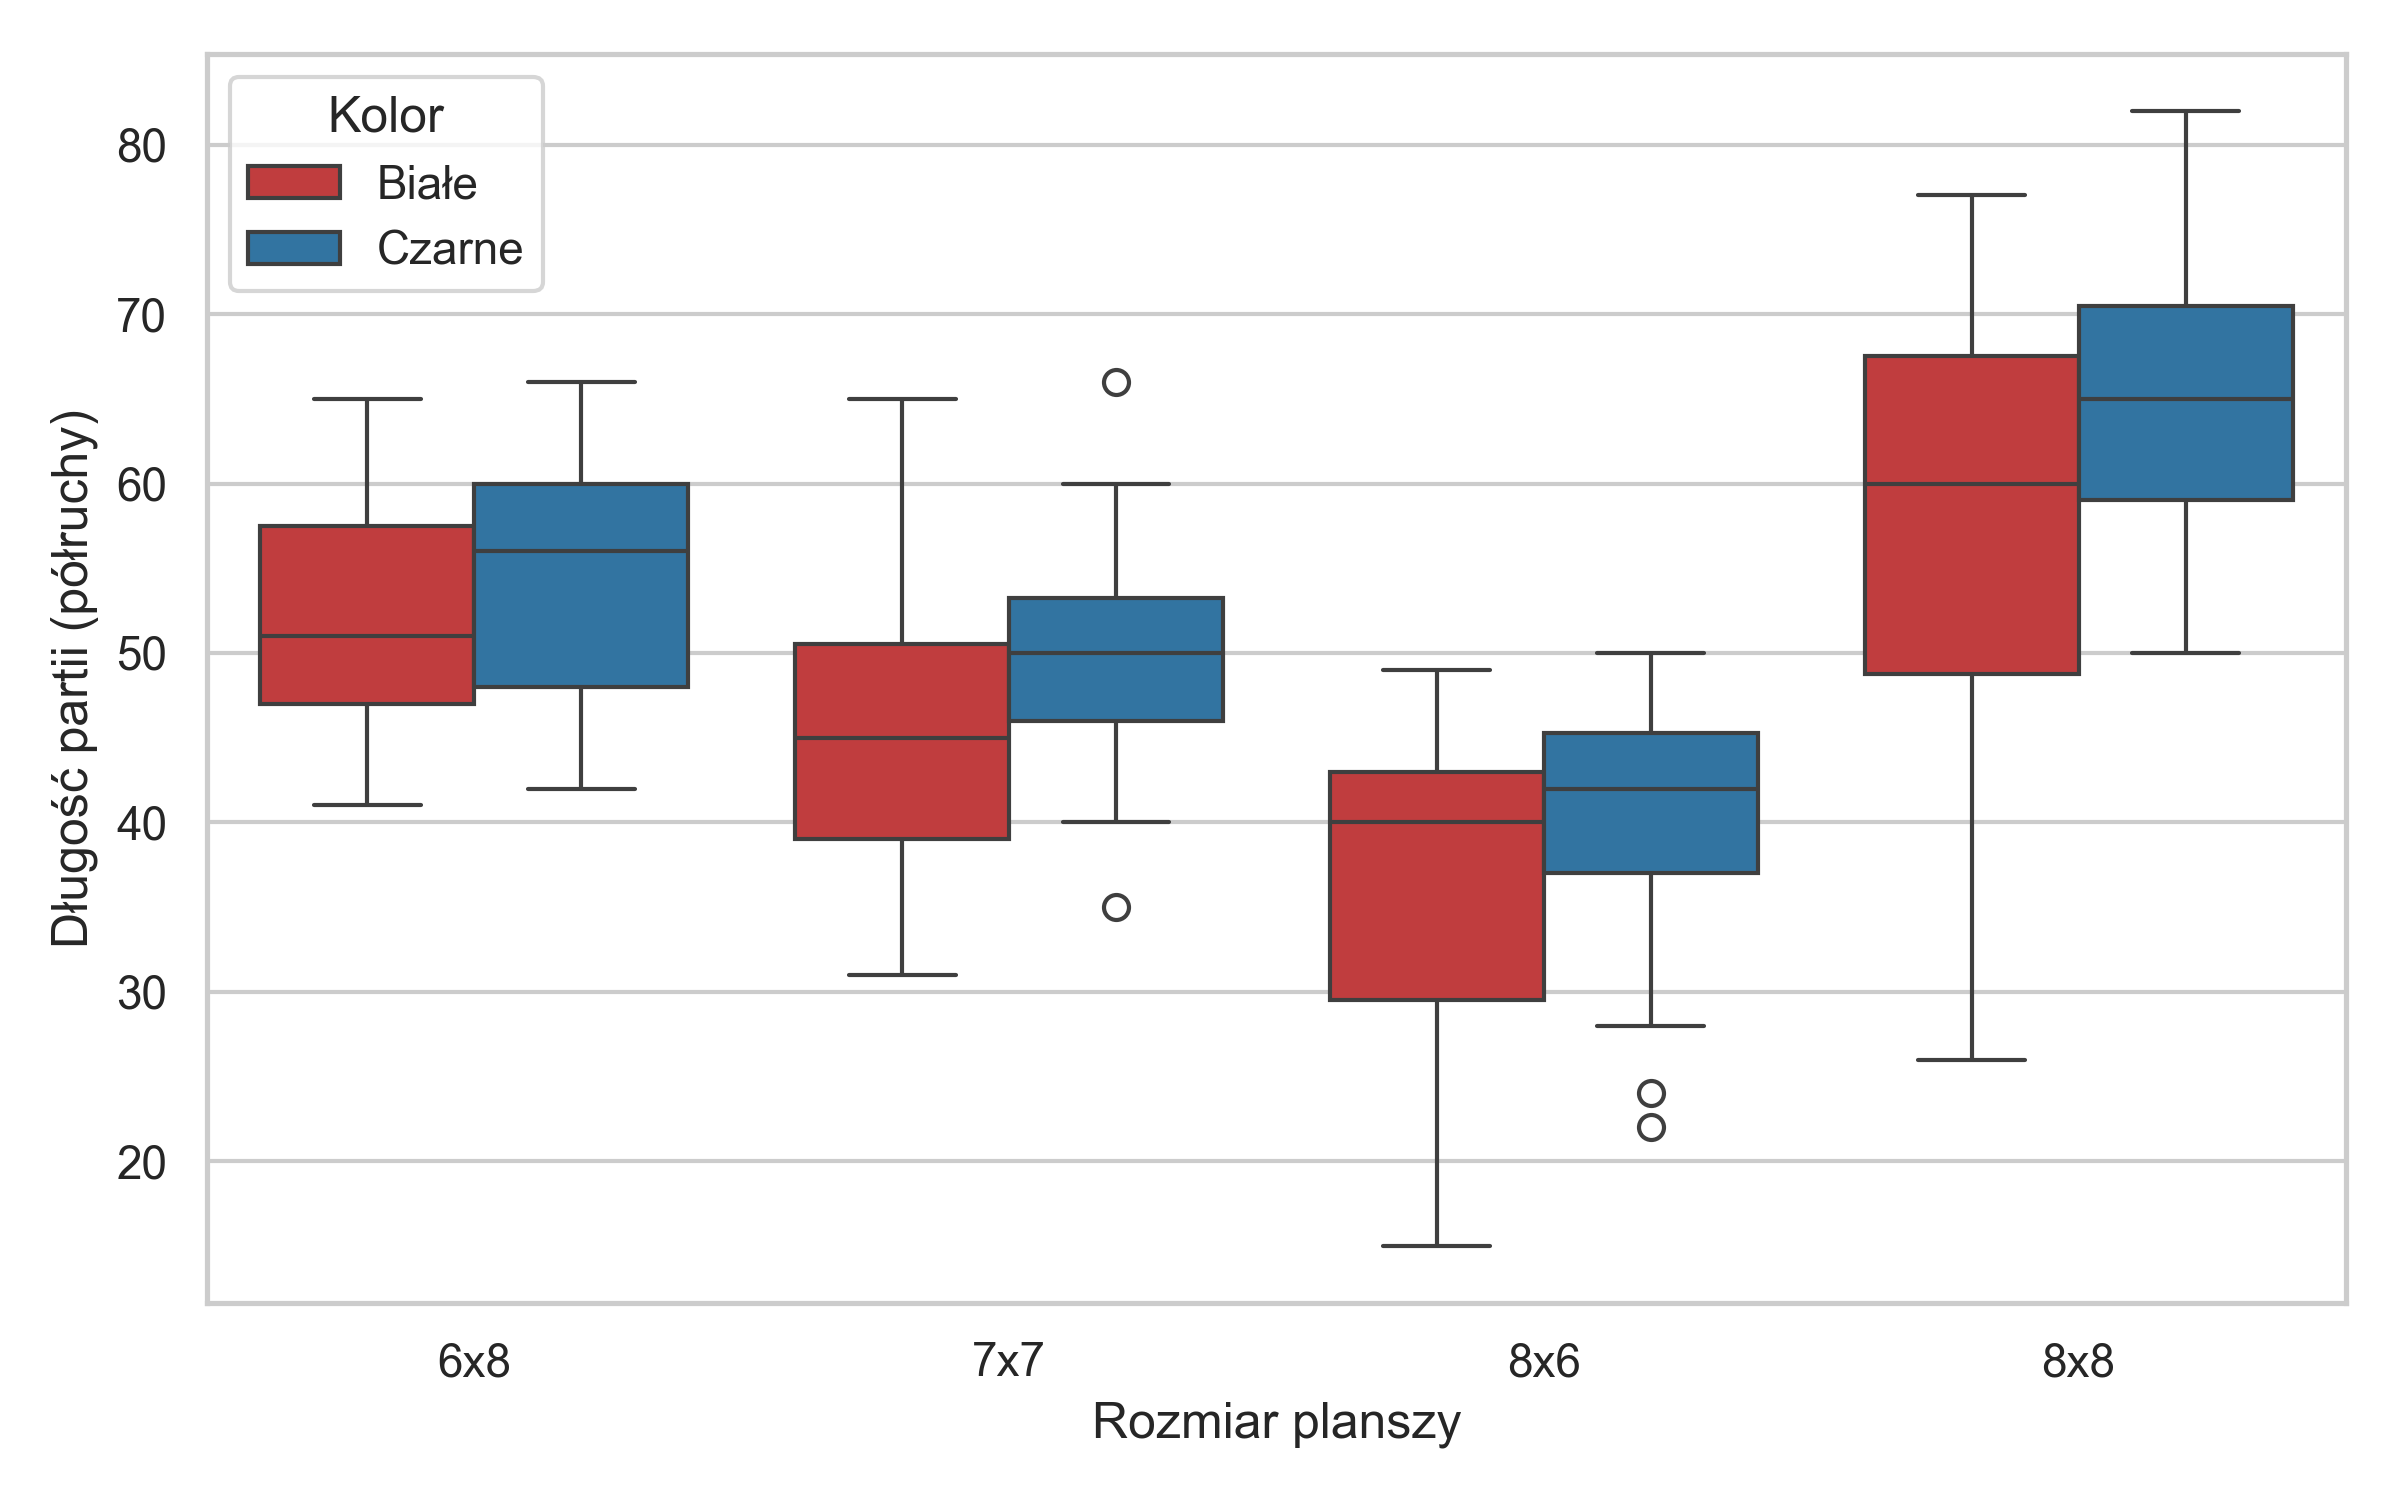
\includegraphics[width=\textwidth]{images/h2_game_length_by_board_and_color.png}
        \caption{Rozkład długości partii}
        \label{fig:h2-game-length}
    \end{subfigure}

    \caption{Dodatkowe charakterystyki eksperymentu H2: koszt obliczeniowy oraz długość partii.}
    \label{fig:h2-additional}
\end{figure}

\noindent
Na wszystkich badanych rozmiarach plansz widoczna jest wyraźna asymetria długości gry w zależności od koloru kontrolowanego przez agenta Heavy Playouts (Rysunek~\ref{fig:h2-game-length}). Partie, w których wariant heurystyczny grał czarnymi, były konsekwentnie dłuższe od partii, w których grał białymi. Jak wspomniano wcześniej, w grze Breakthrough białe posiadają naturalną przewagę pierwszego ruchu. W tym eksperymencie dłuższa rozgrywka po stronie czarnej może jednak wynikać z faktu, że Heavy Playouts skuteczniej opóźniał postęp przeciwnika dzięki trafniejszej ewaluacji defensywnej podczas symulacji. Wydłużało to czas trwania partii, pozwalając agentowi zneutralizować inicjatywę białych i częściej wygrywać w późniejszej fazie gry.

\subsubsection{Wnioski końcowe}

\textbf{Hipoteza H2 zostaje przyjęta}. Przy limicie 250 ms na ruch agent MCTS + Heavy Playouts osiągnął 90.6\% zwycięstw w bezpośrednim starciu z bazowym MCTS, wyraźnie przekraczając wymagany próg 55\%. Wyniki eksperymentu wskazują, że w grze Breakthrough podniesienie jakości pojedynczej symulacji poprzez wprowadzenie wiedzy domenowej kompensuje straty wynikające ze zwiększonego czasu obliczeń i mniejszego rozmiaru generowanego drzewa gry. Mimo że agent wykonuje mniej iteracji, informacje płynące z każdej symulacji są bardziej wartościowe. Heurystyka w fazie \textit{playout} lepiej odzwierciedla zachowania istotne strategicznie: bicie pionów przeciwnika, ochronę własnych pionów oraz unikanie niekorzystnych pozycji na krawędziach planszy. Na podstawie tak ukierunkowanych symulacji agent podejmuje decyzje wyraźnie skuteczniejsze niż klasyczny MCTS.

\newpage
\subsection{Hipoteza 3: Przewaga nad ewaluacją statyczną}

\subsubsection{Metodologia i przebieg eksperymentu}

Weryfikacja hipotezy wymagała przeprowadzenia serii rozgrywek turniejowych, w których zautomatyzowani agenci bazujący na algorytmie MCTS zostali skonfrontowani z agentem heurystycznym, wykorzystującym algorytm Minimax ze statyczną funkcją oceny pozycji. Celem eksperymentu było zbadanie, czy probabilistyczne podejście do przeszukiwania przestrzeni stanów pozwala na uzyskanie przewagi nad deterministycznym oponentem o ograniczonym horyzoncie planowania.

Eksperyment podzielono na trzy główne serie pomiarowe, odpowiadające testowanym wariantom algorytmu sterującego: MCTS, MCTS + RAVE oraz MCTS + Heavy Playouts. W każdej z serii agent testowy (korzystający ze stałego budżetu iteracyjnego 10000) rozgrywał partie przeciwko agentowi Minimax. Siła oponenta była stopniowo zwiększana poprzez inkrementację limitu maksymalnej głębokości przeszukiwania drzewa gry (parametr $d$) w przedziale od $d=1$ do $d=7$. Pozwoliło to na weryfikację zachowania wariantów stochastycznych w starciu z przeciwnikiem o rosnących zdolnościach taktycznych.

Dla każdej testowanej głębokości oponenta rozegrano 20 niezależnych partii. Aby zneutralizować wpływ przewagi pierwszego ruchu, zrezygnowano z przypisywania stałych ról –- w 10 partiach agent kontrolował piony białe, a w pozostałych 10 piony czarne. Tym samym każda z trzech serii pomiarowych składała się ze 140 partii, co przełożyło się na 420 rozegranych gier w całym eksperymencie.

Zgodnie z przyjętymi założeniami, główną metryką decydującą o weryfikacji hipotezy H3 był sumaryczny odsetek wygranych partii (wymagany próg powyżej 70\%). Dodatkowo, w celu pogłębienia analizy, z zebranych logów wyodrębniono informacje na temat średniej długości trwania rozgrywki (liczby ruchów) oraz czasów namysłu poszczególnych algorytmów.

\subsubsection{Analiza wyników}

Zestawienie odsetka wygranych partii dla wszystkich trzech wariantów algorytmu MCTS (MCTS, MCTS + RAVE oraz MCTS + Heavy Playouts) w zależności od głębokości przeszukiwania agenta Minimax przedstawiono na Rysunku~\ref{fig:comparison-winrate} oraz w Tabeli \ref{tab:comparison-win-rate}. \\

\begin{figure}[H]
    \centering

    \begin{subfigure}[b]{0.49\textwidth}
        \centering
        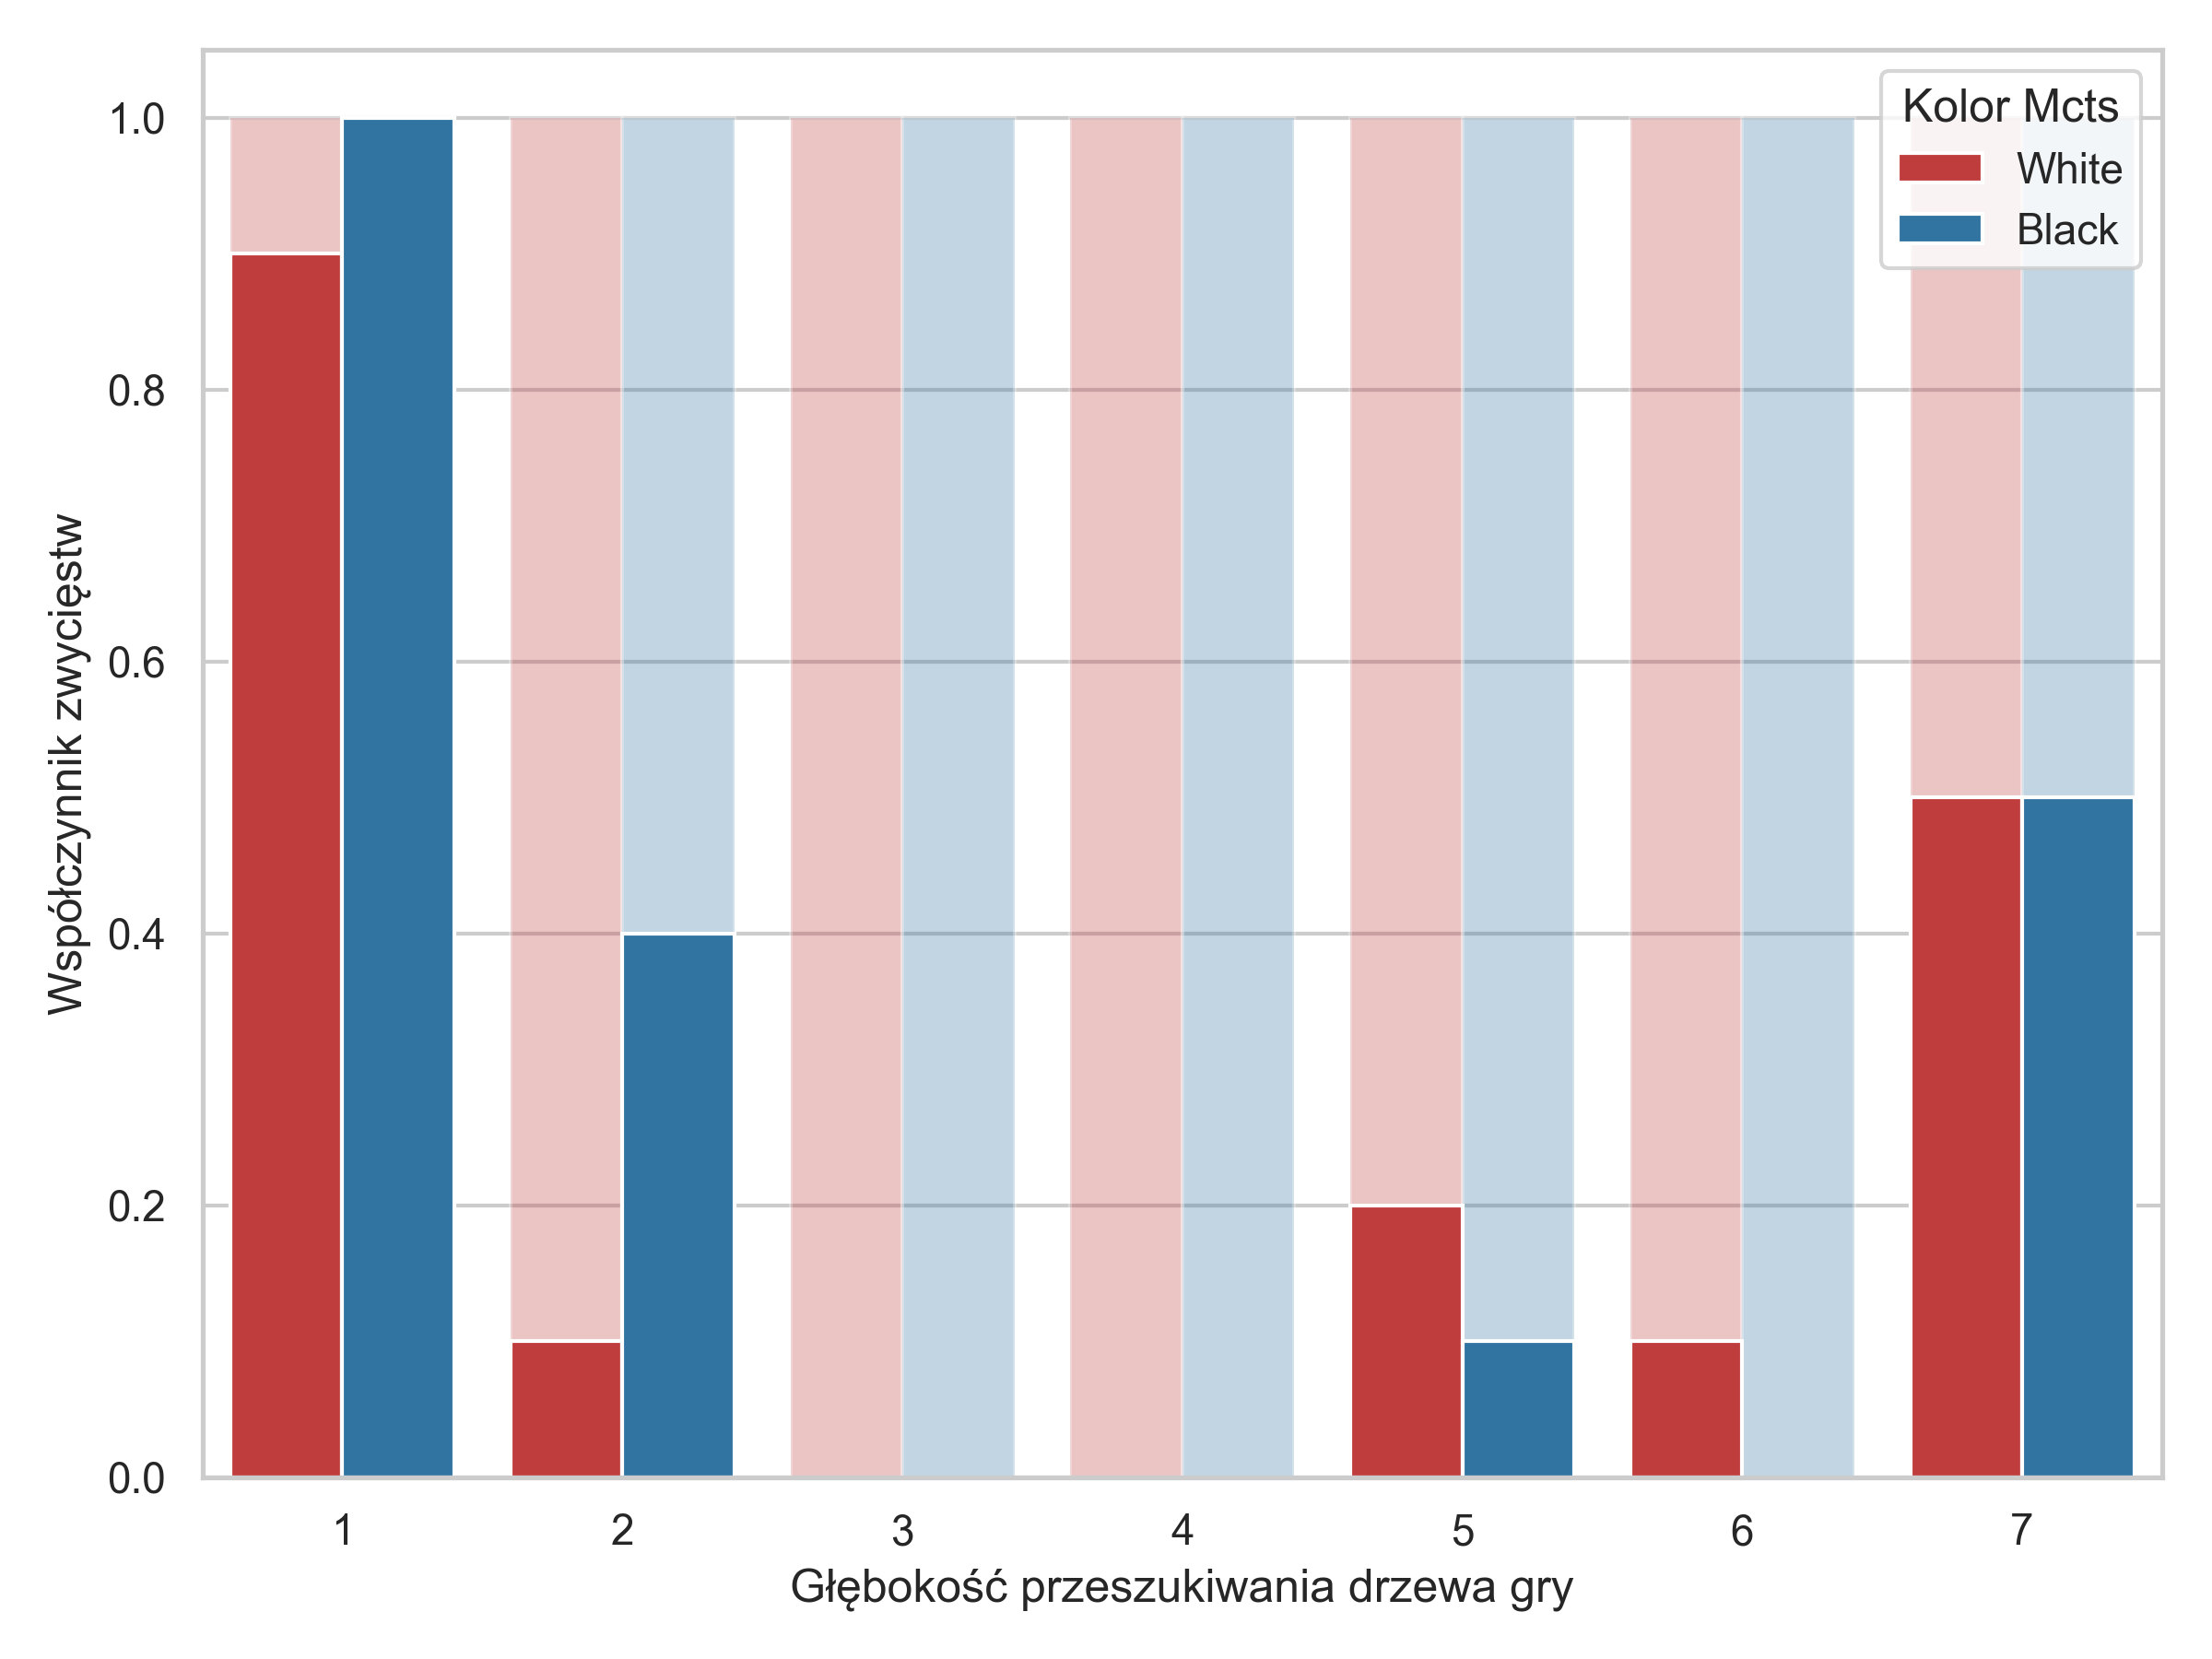
\includegraphics[width=\textwidth]{images/mcts_win_rate.png}
        \caption{Klasyczny MCTS}
        \label{fig:winrate-mcts}
    \end{subfigure}
    \hfill
    \begin{subfigure}[b]{0.49\textwidth}
        \centering
        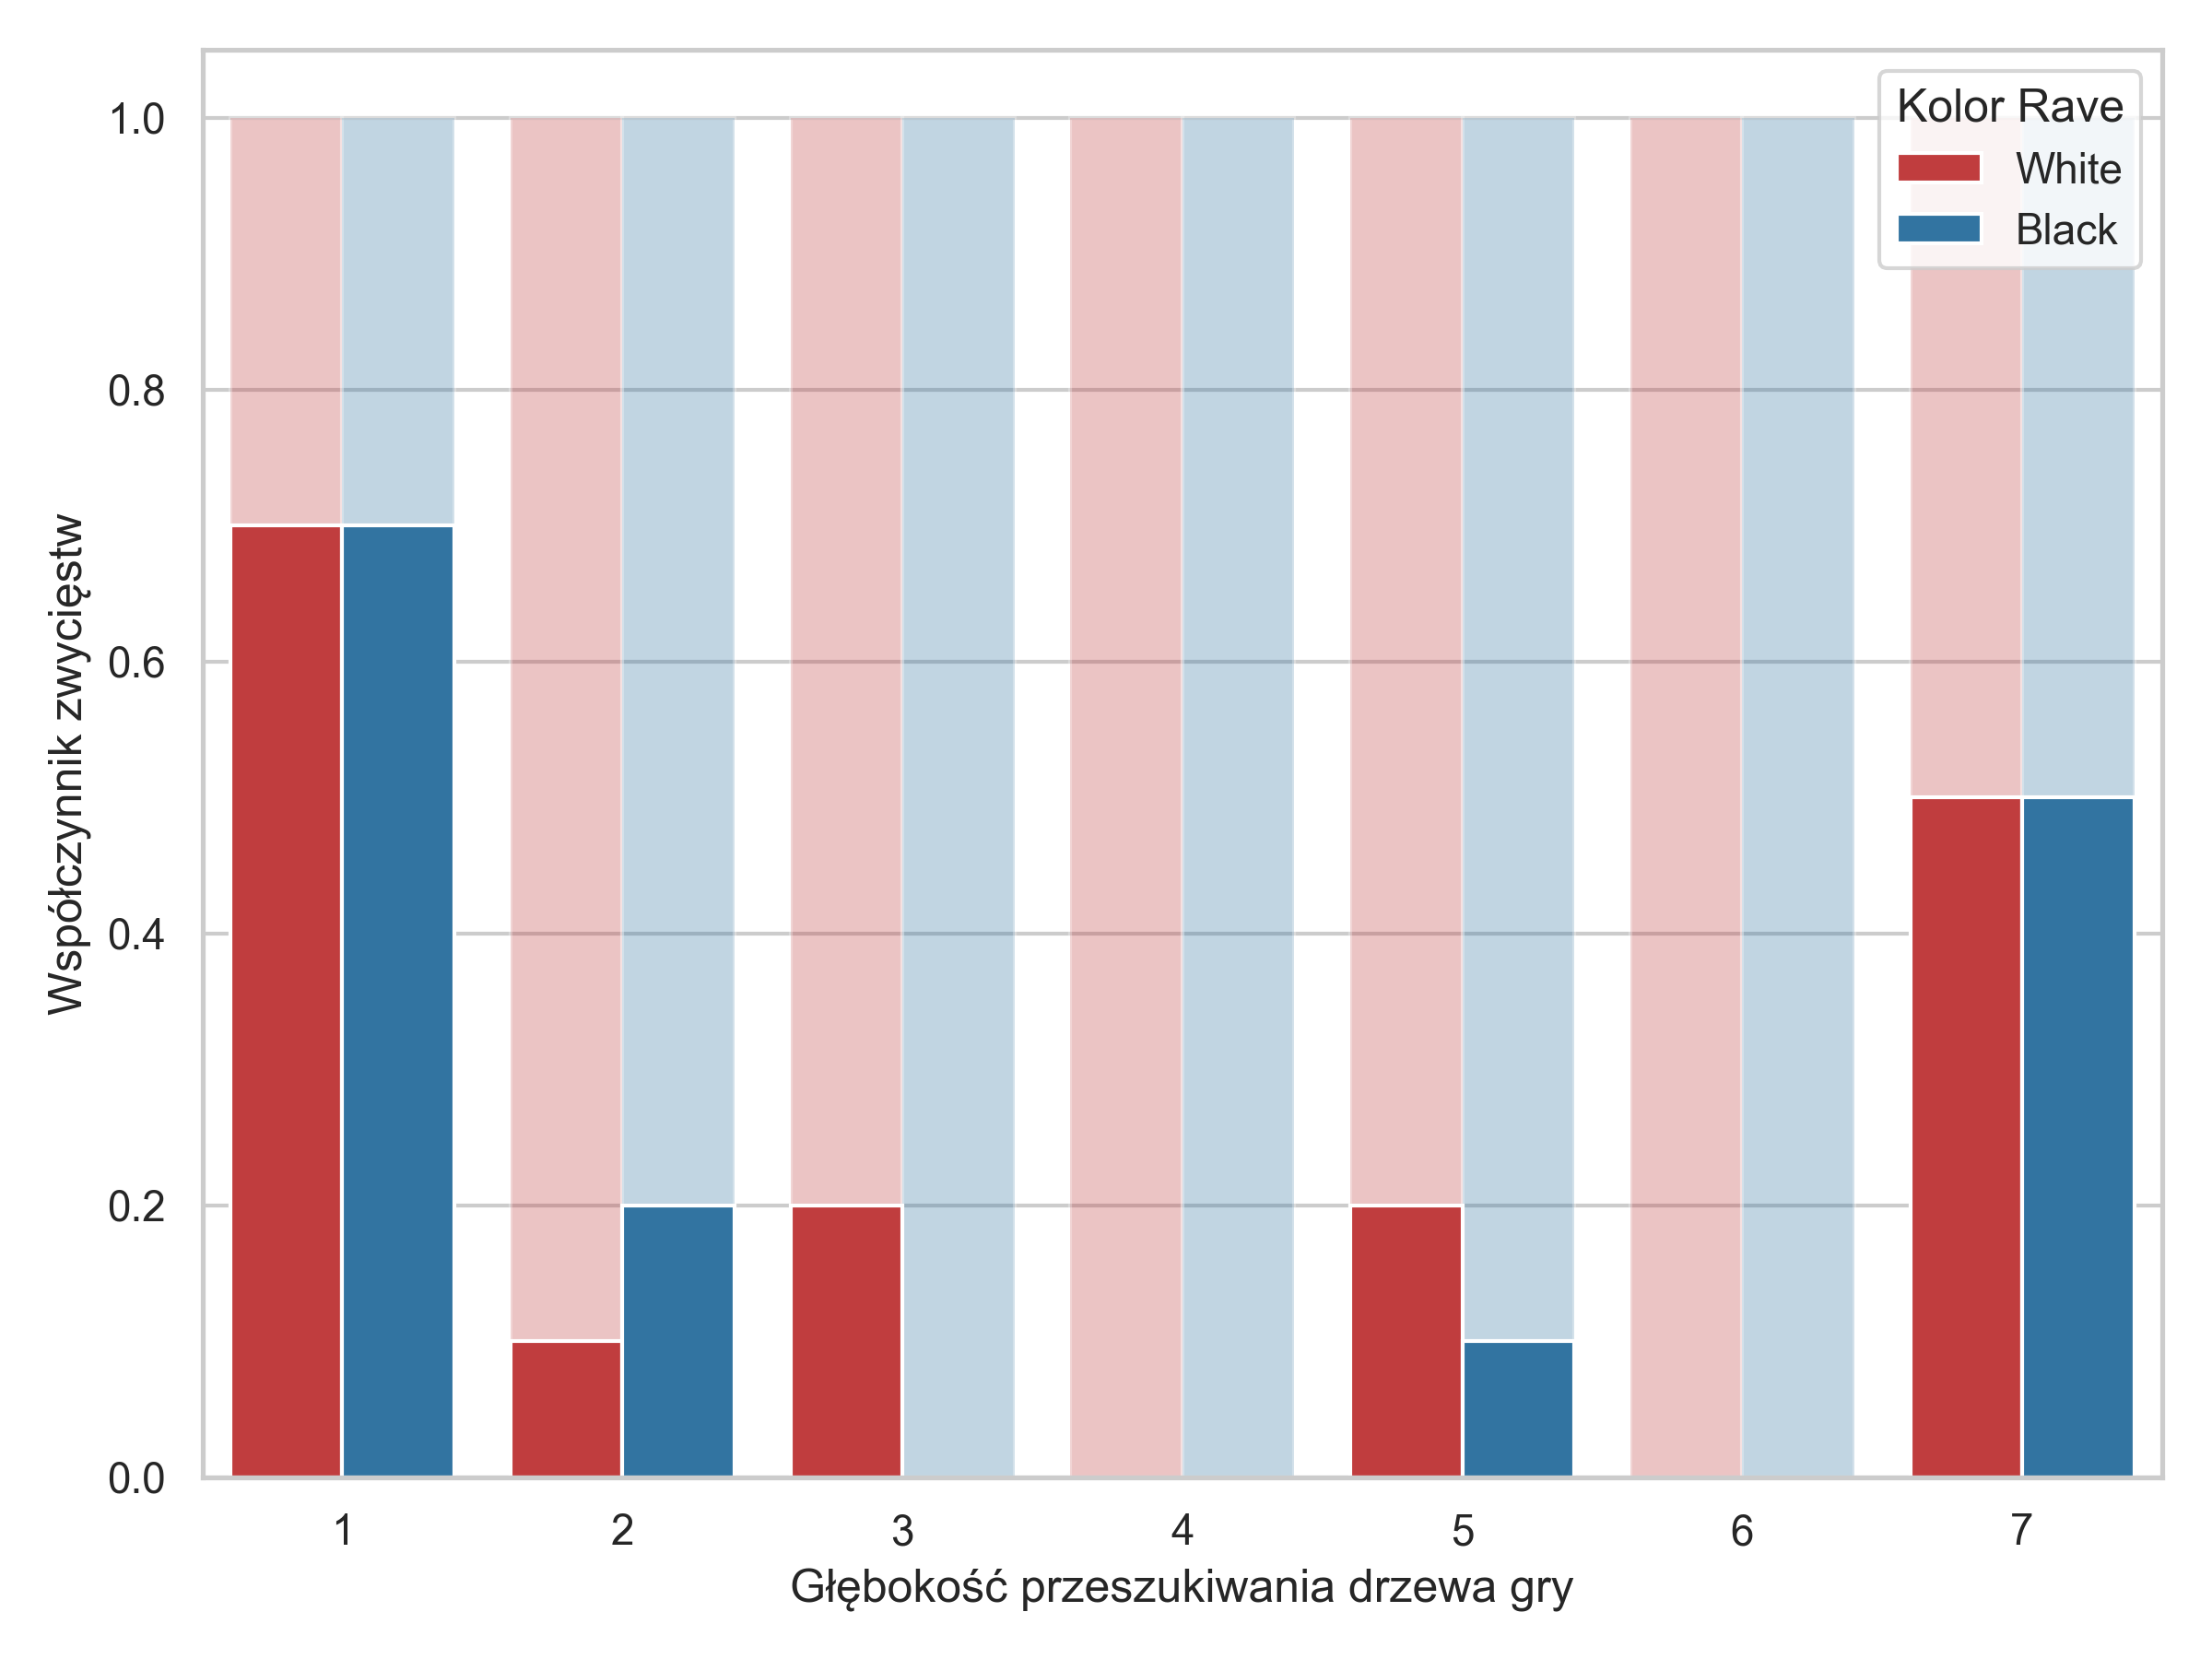
\includegraphics[width=\textwidth]{images/rave_win_rate.png}
        \caption{MCTS + RAVE}
        \label{fig:winrate-rave}
    \end{subfigure}

    \vspace{0.5cm}

    \begin{subfigure}[b]{0.49\textwidth}
        \centering
        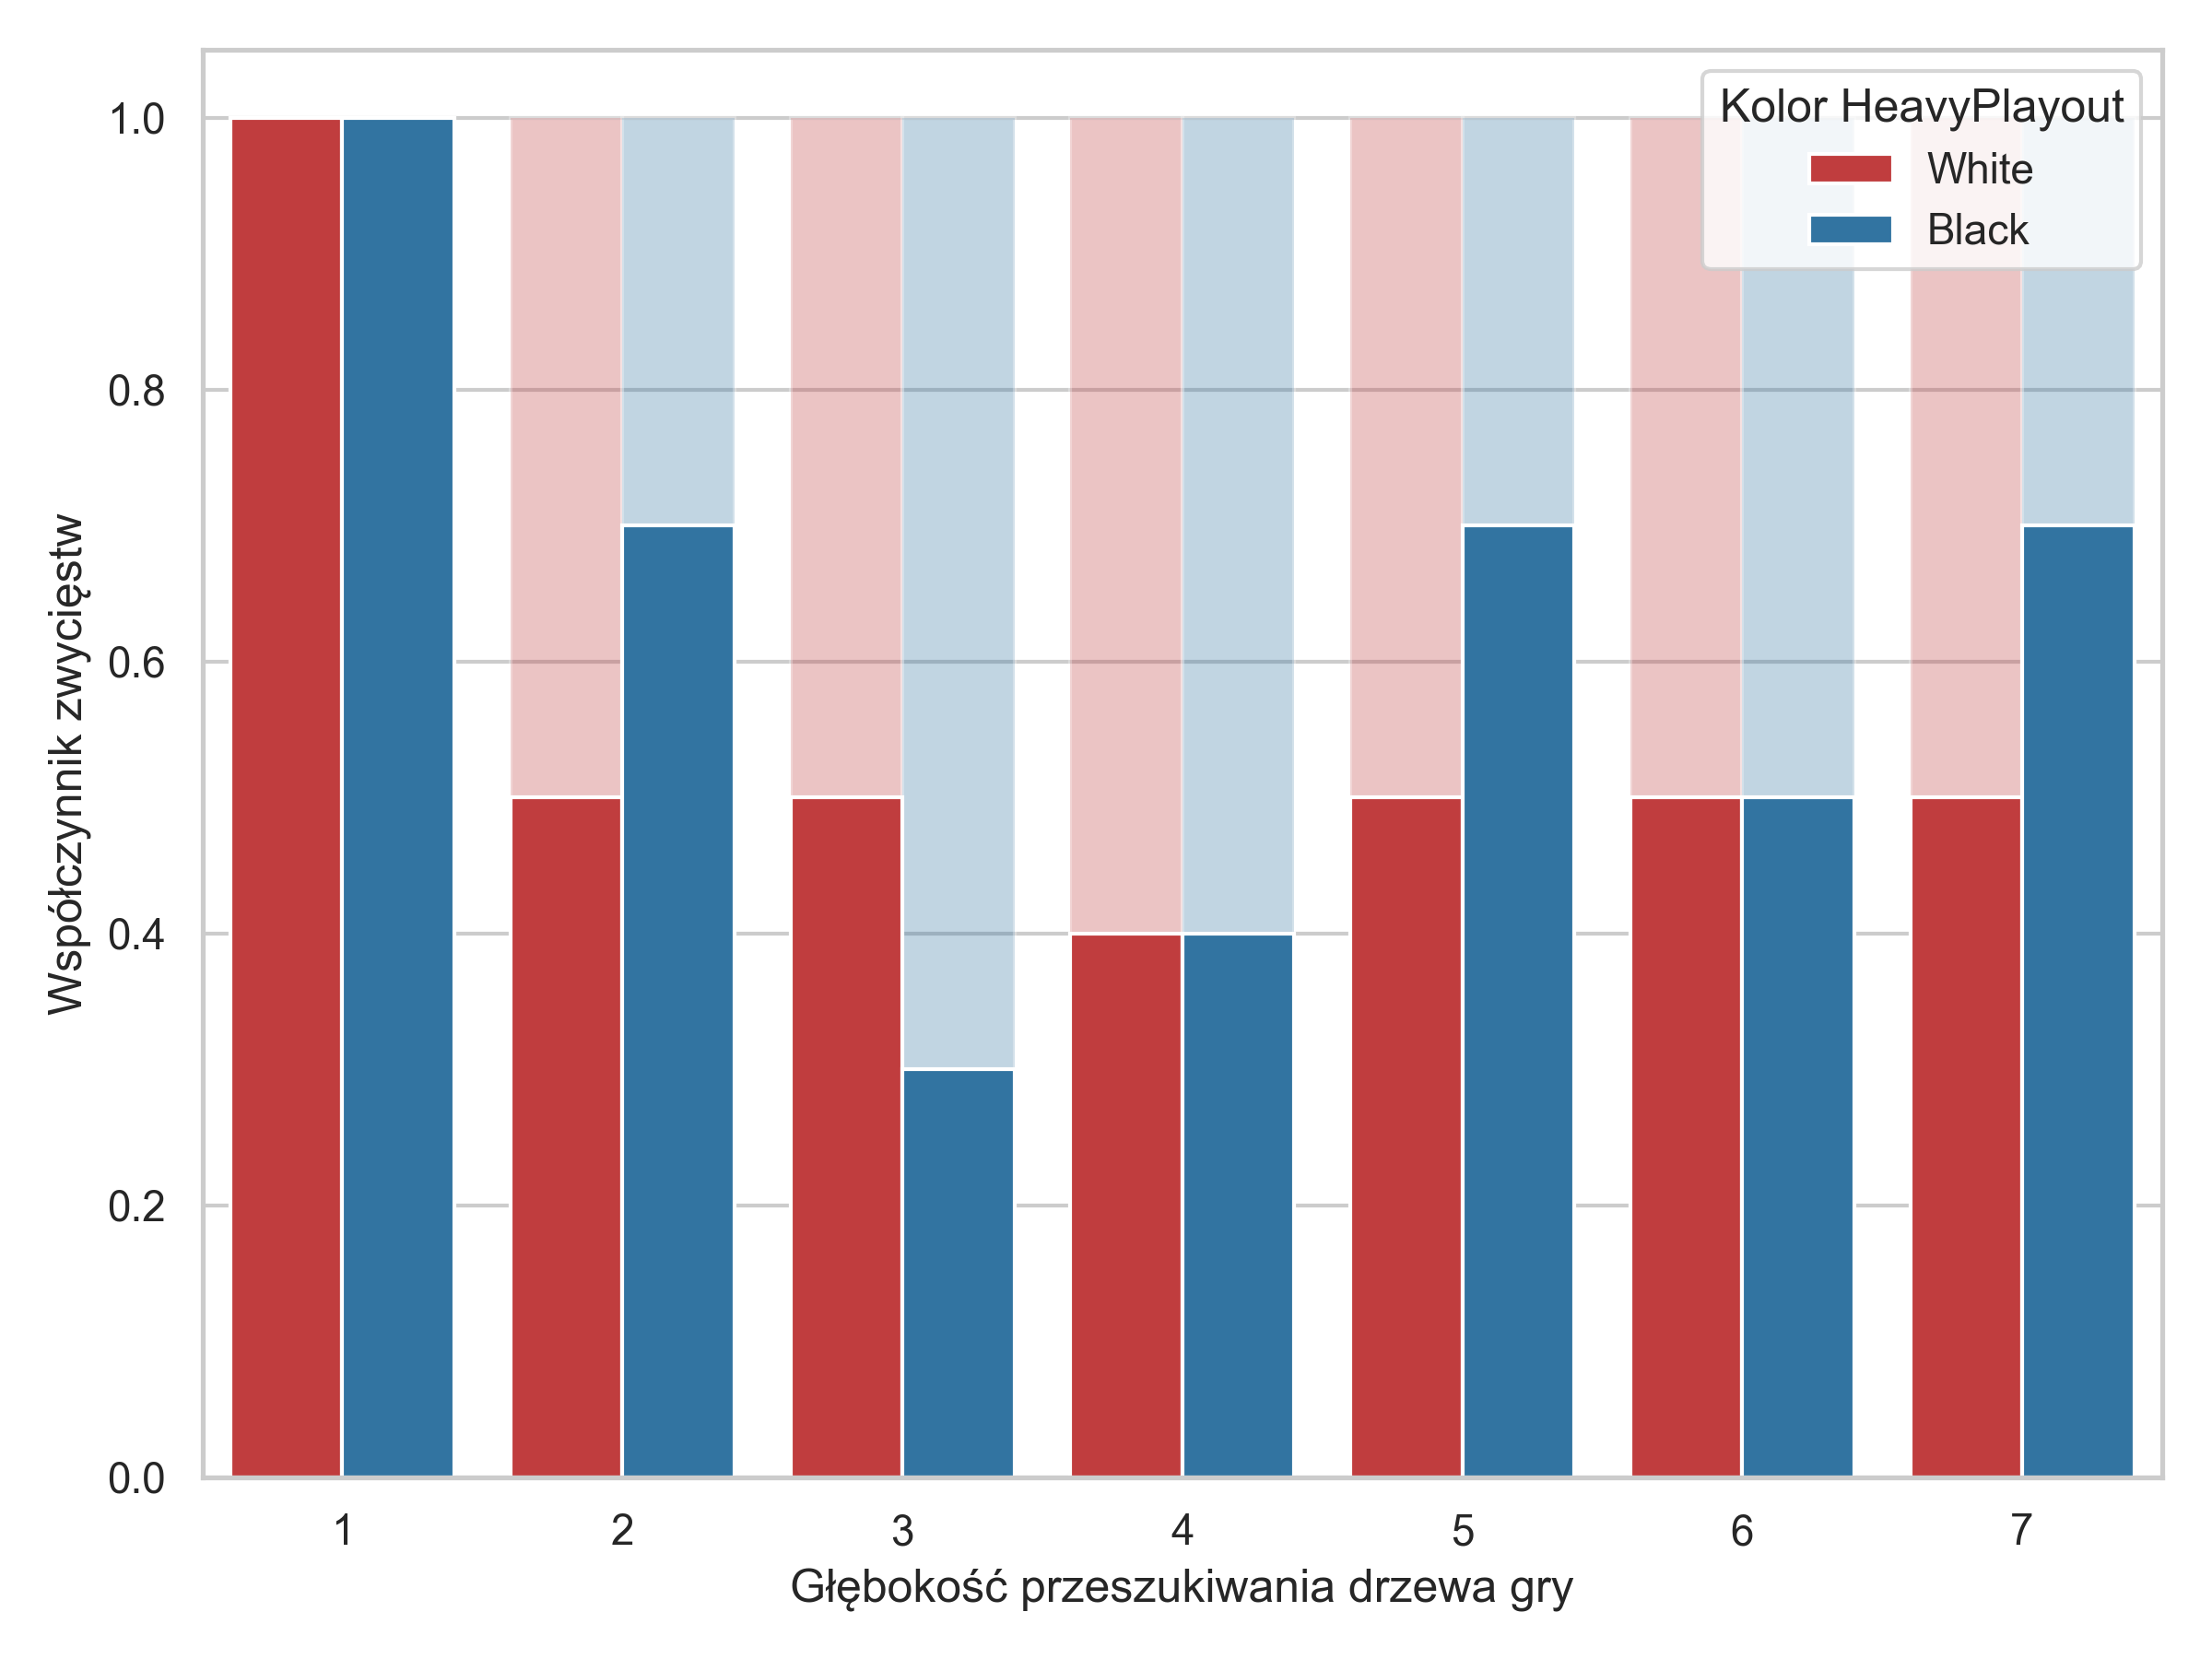
\includegraphics[width=\textwidth]{images/heavyplayouts_win_rate.png}
        \caption{MCTS + Heavy Playouts}
        \label{fig:winrate-heavy}
    \end{subfigure}

    \caption{Porównanie odsetka wygranych partii w zależności od głębokości przeszukiwania agenta Minimax dla różnych wariantów algorytmu MCTS.}
    \label{fig:comparison-winrate}
\end{figure}

\noindent
Bezpośrednie porównanie tych wykresów pozwala na sformułowanie kilku obserwacji dotyczących stabilności i siły gry poszczególnych modyfikacji:

\begin{enumerate}
    \item Niezależnie od zastosowanego wariantu MCTS, można zaobserwować wyraźny trend spadku skuteczności w początkowej fazie wykresu. Dla najmniejszej głębokości ($d=1$), wszystkie modyfikacje oparte na symulacjach całkowicie dominują agenta Minimax, osiągając wskaźniki zwycięstw bliskie lub równe 100\% ($\geq 70\%)$. Jednakże, wraz ze wzrostem limitu głębokości do $d=3$ i $d=4$, siła gry Minimaxa znacząco rośnie, co przekłada się na gwałtowny spadek skuteczności agentów probabilistycznych. W tym przedziale klasyczny MCTS oraz MCTS z modyfikacją RAVE przegrywają niemal wszystkie partie, co obnaża podatność losowych oraz pół-losowych symulacji na szerszy horyzont planowania agenta Minimax
    \item Szczególnie interesujące jest zachowanie algorytmów dla dużych głębokości przeszukiwania oponenta ($d \geq 5$). Na wykresach zauważalne jest swoiste odwrócenie trendu –- skuteczność wariantów MCTS ponownie zaczyna rosnąć, a dla $d=7$ agent Minimax zaczyna regularnie przegrywać z ulepszonymi wariantami (Heavy Playouts i RAVE osiągają lepsze wyniki w tym rejonie w porównaniu do klasycznego MCTS, choć i on odnotowuje wzrost do poziomu około 50\%). Przy bardzo dużych głębokościach (np. $d=7$), agent Minimax staje się ofiarą własnego determinizmu -- ,,ślepo'' ufa zaprogramowanym wagom heurystycznym. Warianty MCTS, dzięki pełnym symulacjom do końca partii, potrafią elastyczniej identyfikować rzeczywiste szanse na wygraną.
    \item Spośród testowanych modyfikacji, wariant MCTS + Heavy Playouts (Rysunek~\ref{fig:winrate-heavy}) wykazał się największą odpornością na siłę taktyczną Minimaxa w środkowym przedziale głębokości ($d=3$, $d=4$).
    \item RAVE (Rysunek~\ref{fig:winrate-rave}) zachowywało się w sposób zbliżony do klasycznego MCTS.
\end{enumerate}

\begin{table}[H]
    \centering
    \caption{Odsetek wygranych partii przez różne warianty algorytmu MCTS w starciu z algorytmami Minimax o zmiennej głębokości przeszukiwania ($d$).}
    \label{tab:comparison-win-rate}
    \renewcommand{\arraystretch}{1.2}

    \begin{tabular}{|c|c|p{1.6cm}|p{3cm}|}
        \hline
        \textbf{Głębokość} & \textbf{MCTS} & \textbf{MCTS + RAVE} & \textbf{MCTS + Heavy Playouts} \\
        \hline
        1 & \hfill 95.0\% & \hfill 70.0\% & \hfill 100.0\% \\
        2 & \hfill 25.0\% & \hfill 15.0\% & \hfill 60.0\% \\
        3 & \hfill 0.0\% & \hfill 10.0\% & \hfill 40.0\% \\
        4 & \hfill 0.0\% & \hfill 0.0\% & \hfill 40.0\% \\
        5 & \hfill 15.0\% & \hfill 15.0\% & \hfill 60.0\% \\
        6 & \hfill 5.0\% & \hfill 0.0\% & \hfill 50.0\% \\
        7 & \hfill 50.0\% & \hfill 50.0\% & \hfill 60.0\% \\
        \hline
    \end{tabular}
\end{table}

\begin{figure}[H]
    \centering

    \begin{subfigure}[b]{0.49\textwidth}
        \centering
        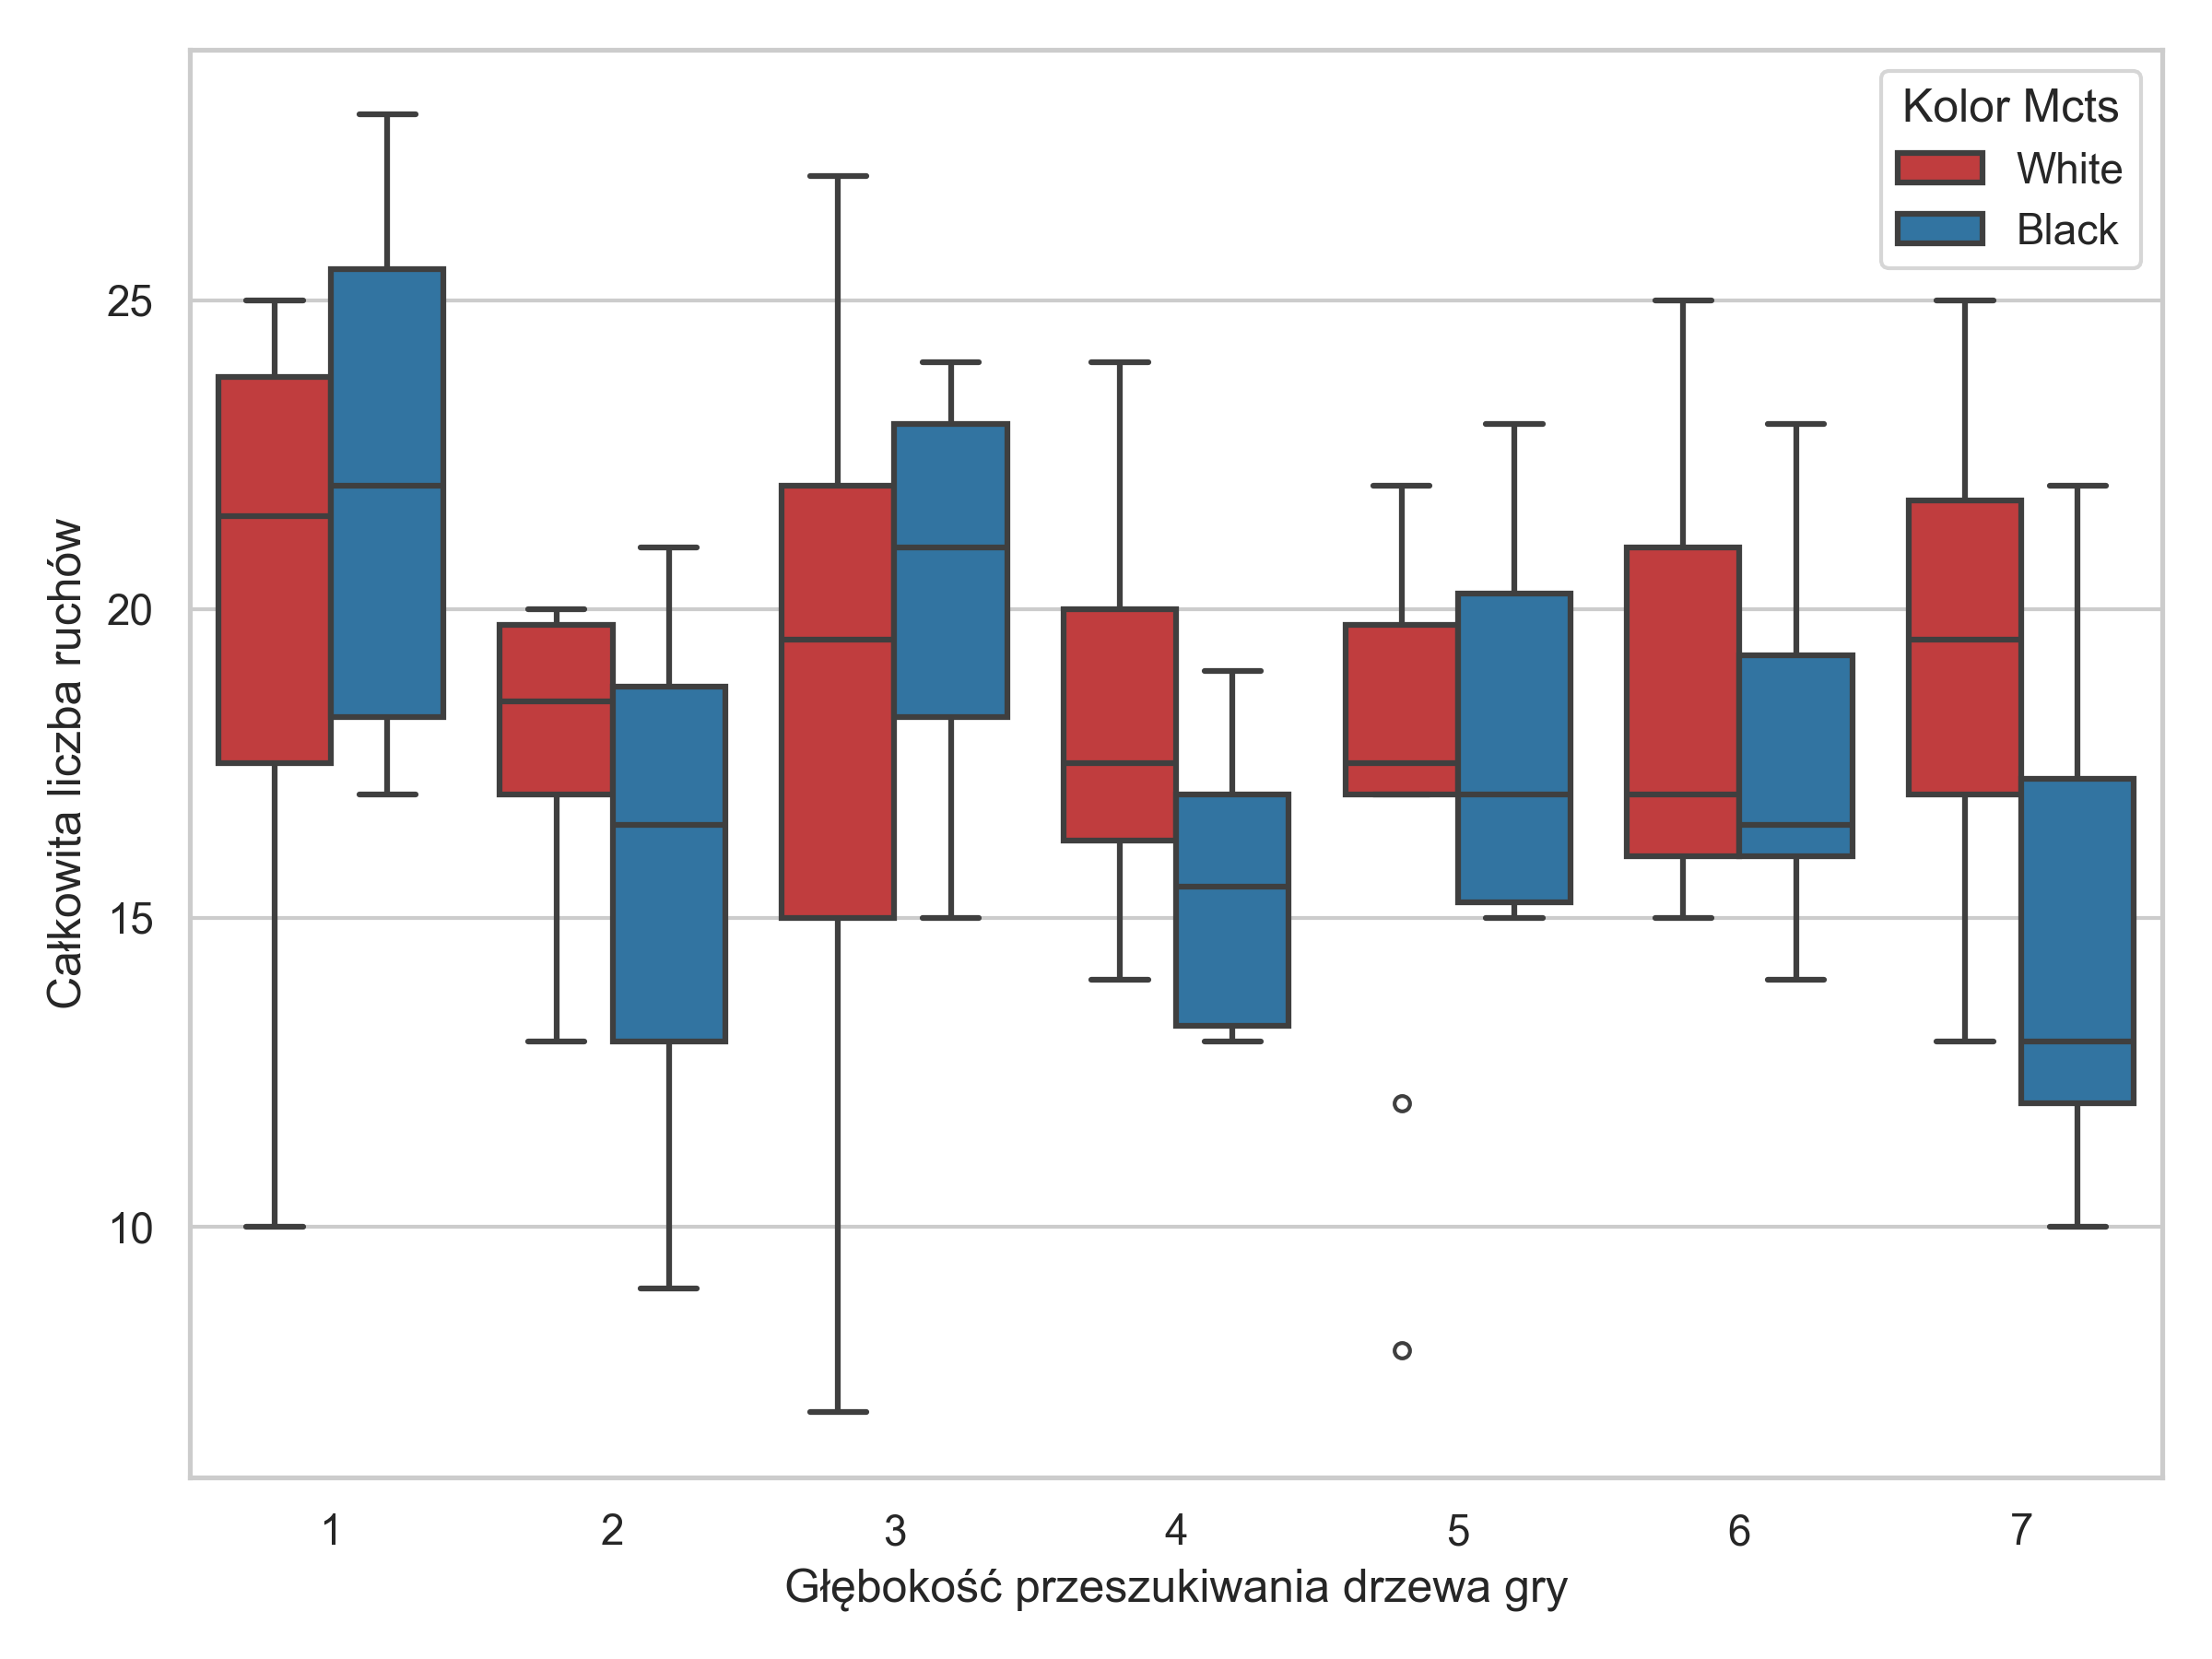
\includegraphics[width=\textwidth]{images/mcts_total_moves.png}
        \caption{Klasyczny MCTS}
        \label{fig:moves-mcts}
    \end{subfigure}
    \hfill
    \begin{subfigure}[b]{0.49\textwidth}
        \centering
        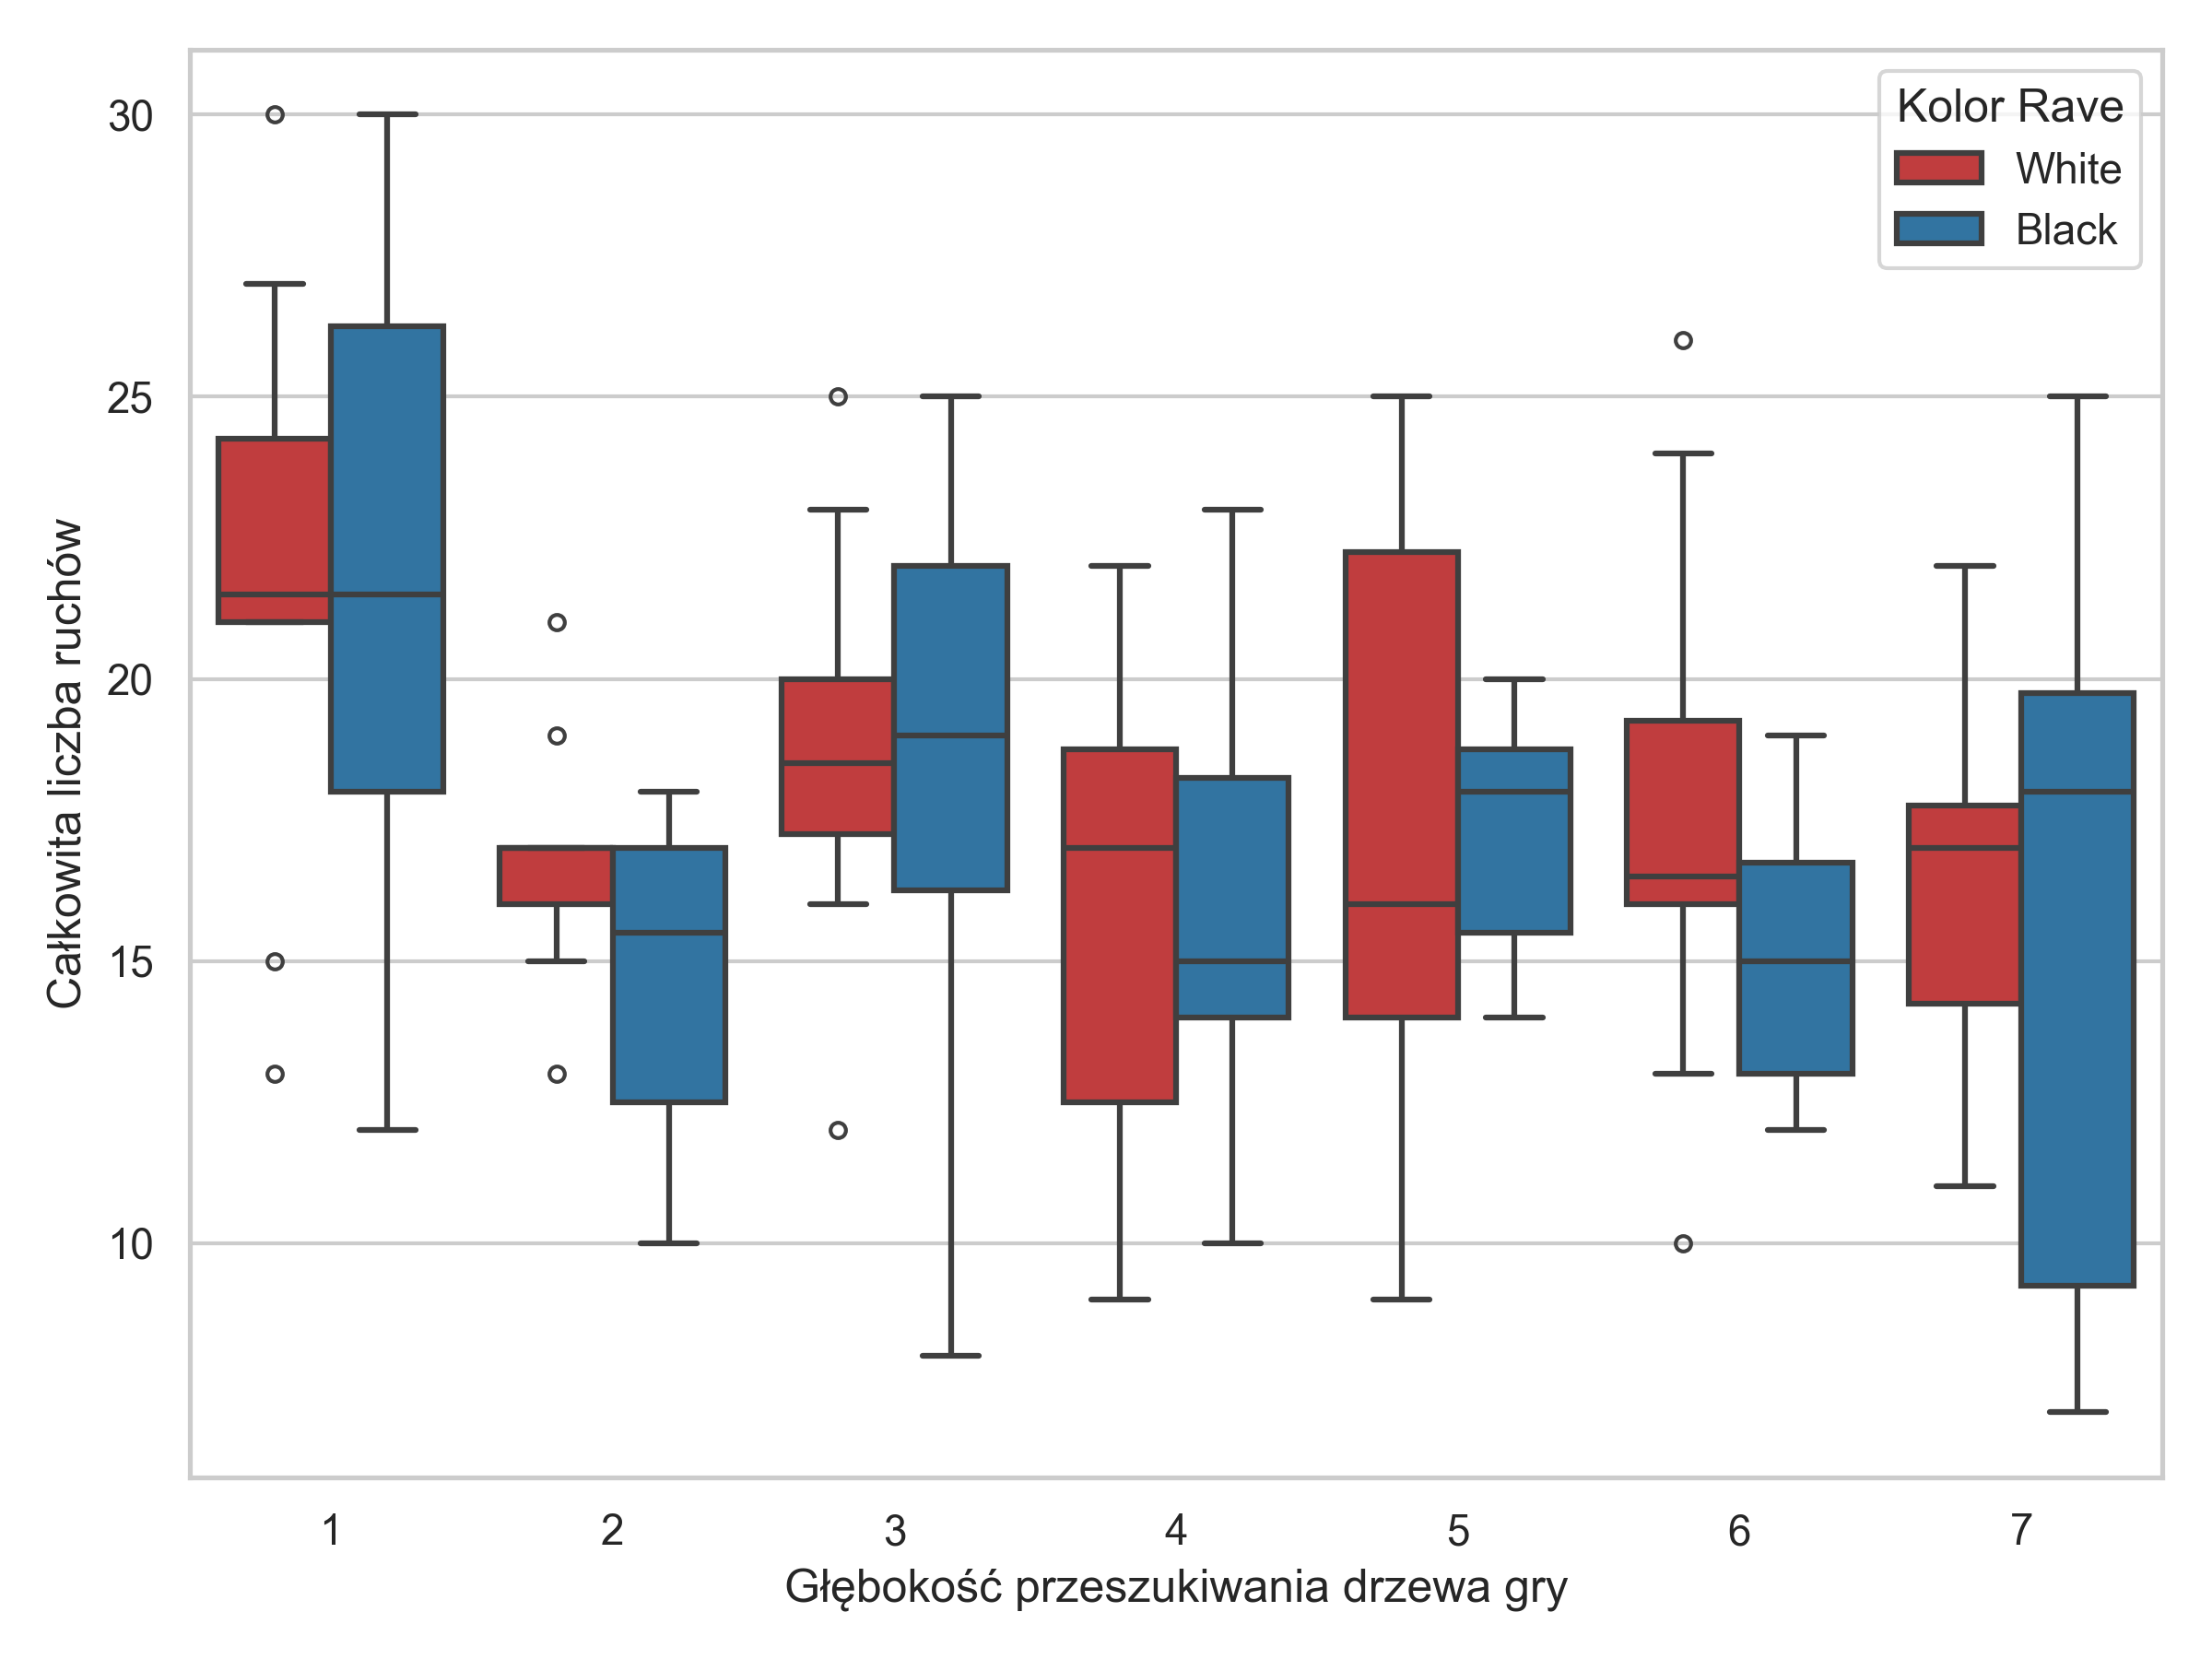
\includegraphics[width=\textwidth]{images/rave_total_moves.png}
        \caption{MCTS + RAVE}
        \label{fig:moves-rave}
    \end{subfigure}

    \vspace{0.5cm}

    \begin{subfigure}[b]{0.49\textwidth}
        \centering
        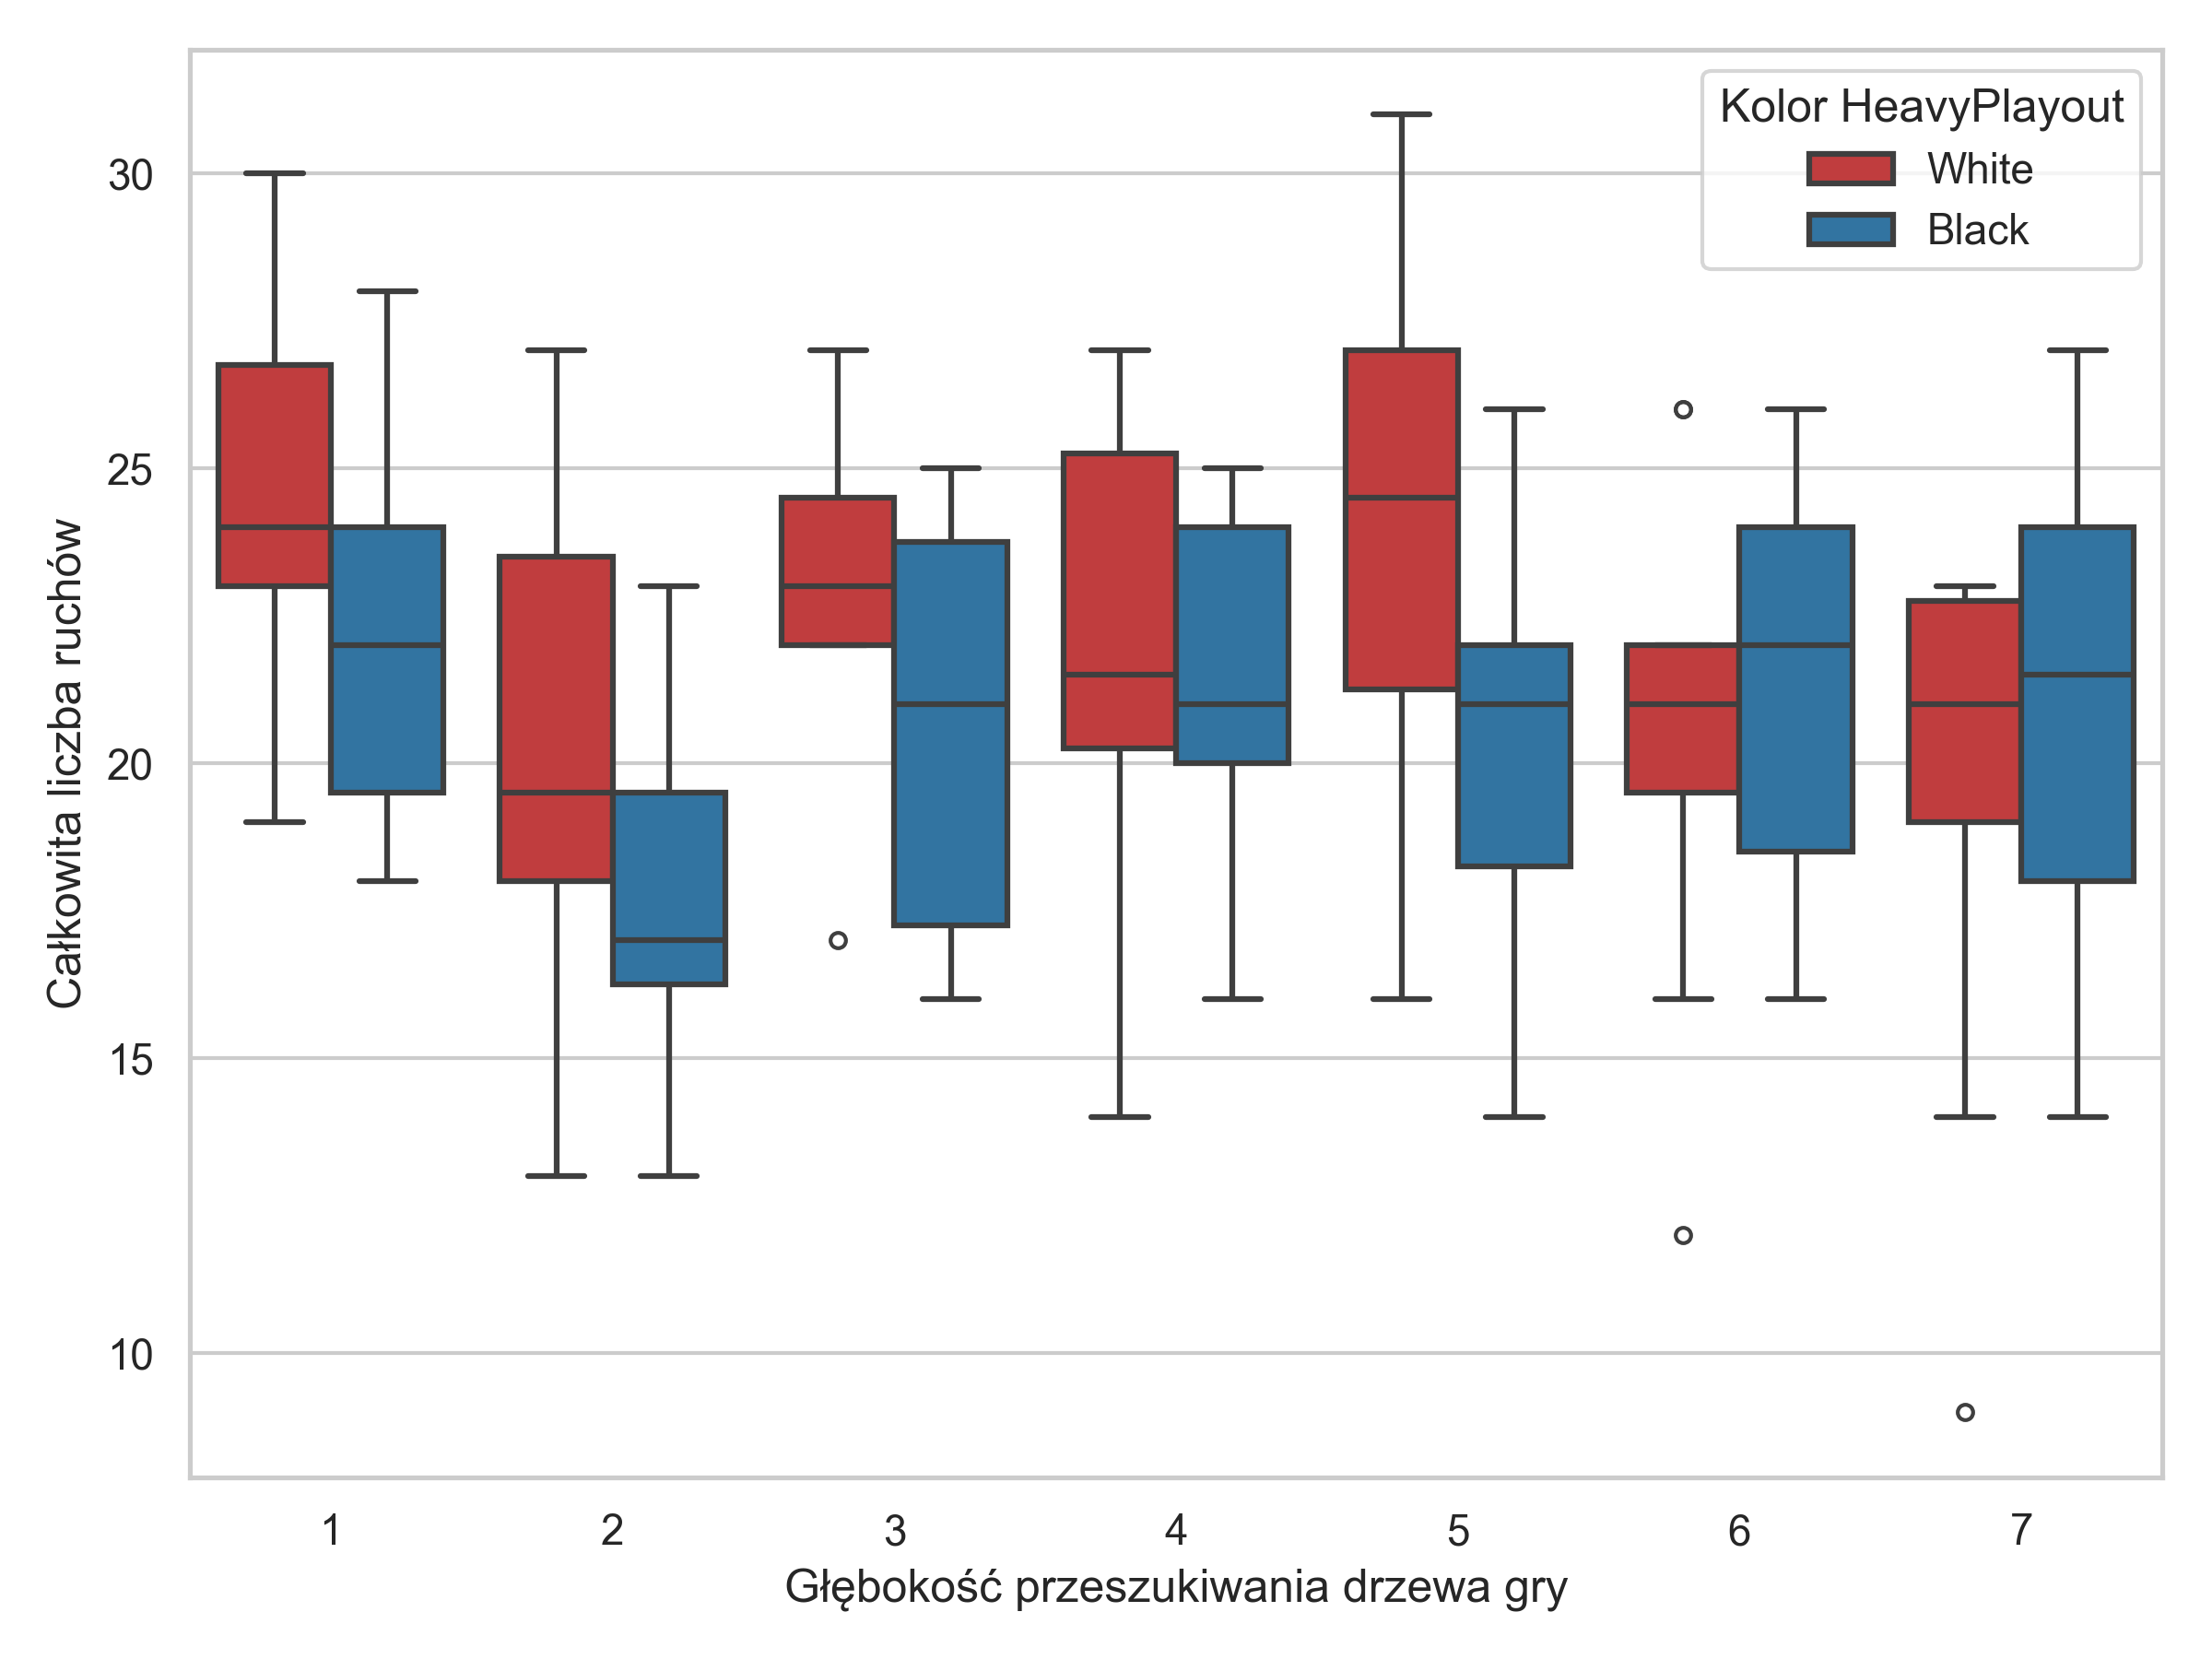
\includegraphics[width=\textwidth]{images/heavyplayouts_total_moves.png}
        \caption{MCTS + Heavy Playouts}
        \label{fig:moves-heavy}
    \end{subfigure}

    \caption{Zestawienie dystrybucji całkowitej liczby ruchów rozegranych w partiach przeciwko agentowi Minimax dla różnych wariantów algorytmu MCTS.}
    \label{fig:comparison-moves}
\end{figure}

\noindent
Kolejnym elementem poddanym analizie była średnia długość rozegranych partii, wyrażona jako całkowita liczba ruchów wykonana przez obu graczy przed osiągnięciem stanu końcowego (Rysunek~\ref{fig:comparison-moves}, Tabela \ref{tab:comparison-game-length}). Wykresy uwzględniają odrębne ,,pudełka'' dla sytuacji, w której agent MCTS steruje bierkami białymi oraz czarnymi.

\begin{table}[H]
    \centering
    \caption{Średnia długość partii (wyrażona jako całkowita liczba ruchów obu graczy) wraz z odchyleniem standardowym, w starciach wariantów MCTS z algorytmem Minimax.}
    \label{tab:comparison-game-length}
    \renewcommand{\arraystretch}{1.2}

    \begin{tabular}{|c|c|p{1.6cm}|p{3cm}|}
        \hline
        \textbf{Głębokość} & \textbf{MCTS} & \textbf{MCTS + RAVE} & \textbf{MCTS + Heavy Playouts} \\
        \hline
        1 & \hfill 21.1 $\pm$ 4.3 & \hfill 21.5 $\pm$ 5.5 & \hfill 23.4 $\pm$ 3.5 \\
        2 & \hfill 17.0 $\pm$ 3.2 & \hfill 15.8 $\pm$ 2.6 & \hfill 19.1 $\pm$ 3.9 \\
        3 & \hfill 19.6 $\pm$ 4.7 & \hfill 18.6 $\pm$ 4.5 & \hfill 21.8 $\pm$ 3.4 \\
        4 & \hfill 16.9 $\pm$ 2.9 & \hfill 16.1 $\pm$ 4.1 & \hfill 21.8 $\pm$ 3.3 \\
        5 & \hfill 17.4 $\pm$ 3.5 & \hfill 17.4 $\pm$ 3.9 & \hfill 22.1 $\pm$ 4.2 \\
        6 & \hfill 17.9 $\pm$ 3.1 & \hfill 16.3 $\pm$ 3.9 & \hfill 21.0 $\pm$ 3.8 \\
        7 & \hfill 17.1 $\pm$ 4.7 & \hfill 15.8 $\pm$ 4.9 & \hfill 20.2 $\pm$ 4.4 \\
        \hline
    \end{tabular}
\end{table}

\begin{figure}[H]
    \centering

    \begin{subfigure}[b]{0.49\textwidth}
        \centering
        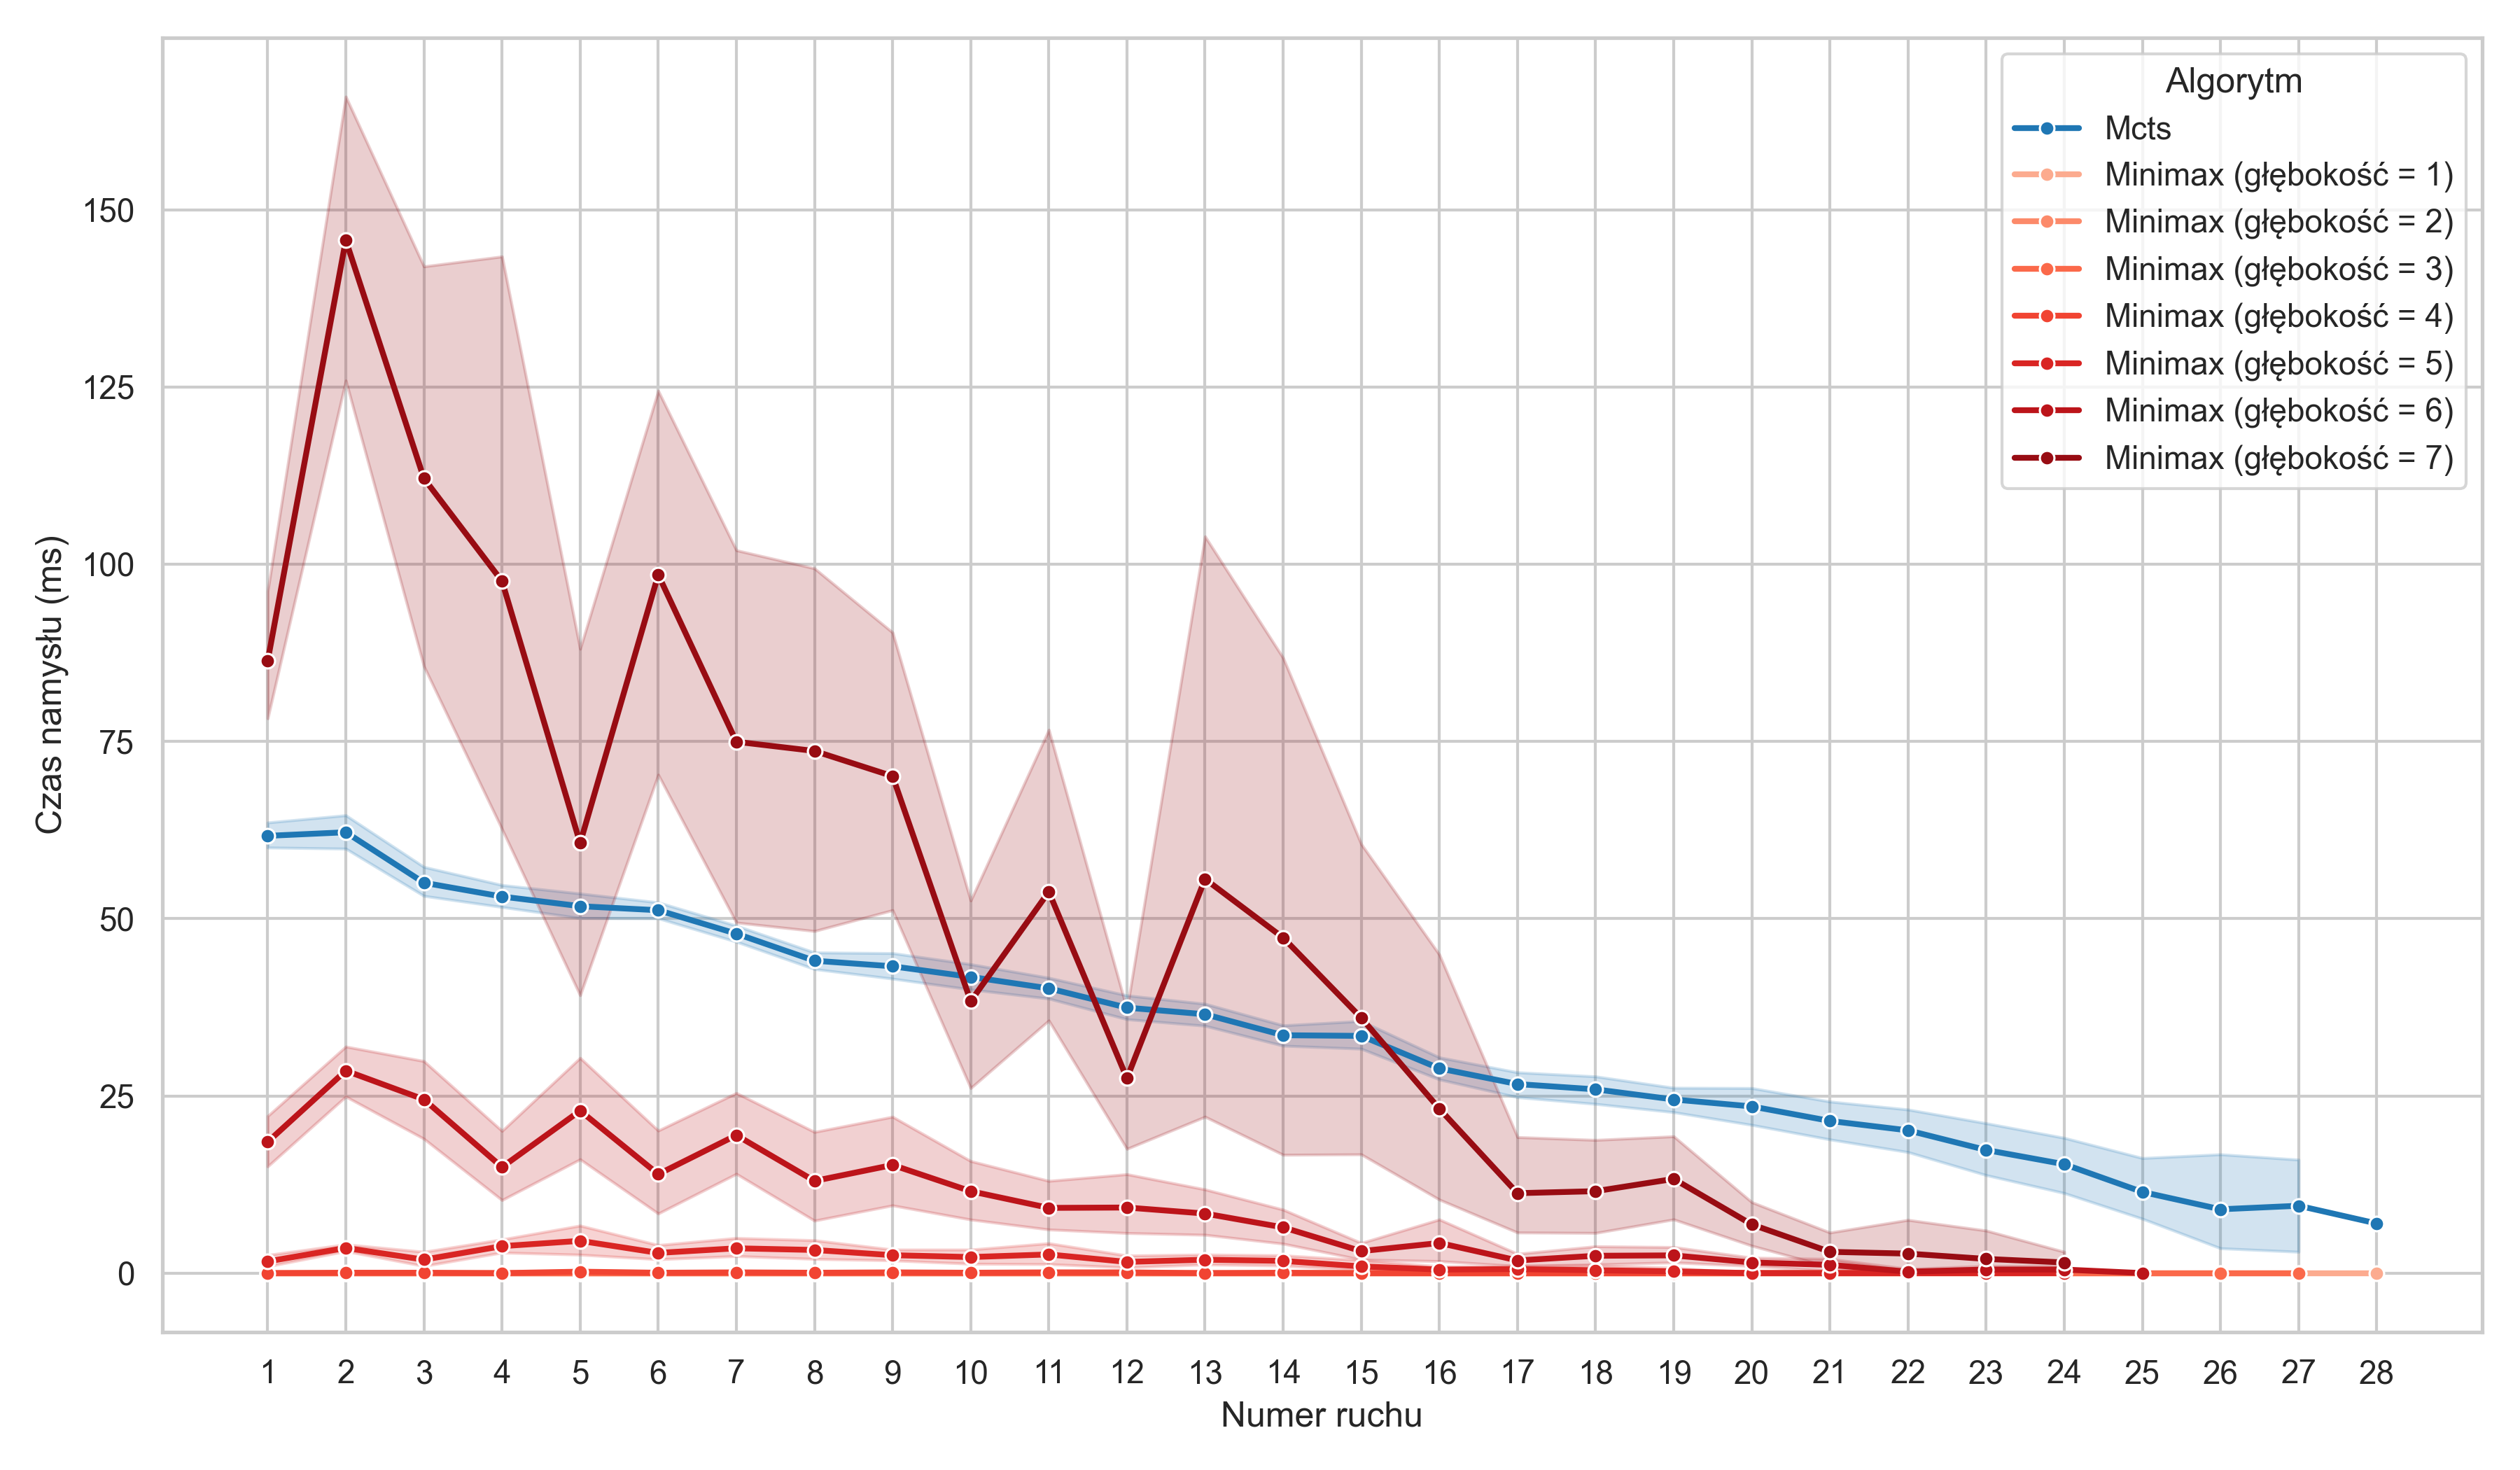
\includegraphics[width=\textwidth]{images/mcts_thinking_time.png}
        \caption{Klasyczny MCTS}
        \label{fig:time-mcts}
    \end{subfigure}
    \hfill
    \begin{subfigure}[b]{0.49\textwidth}
        \centering
        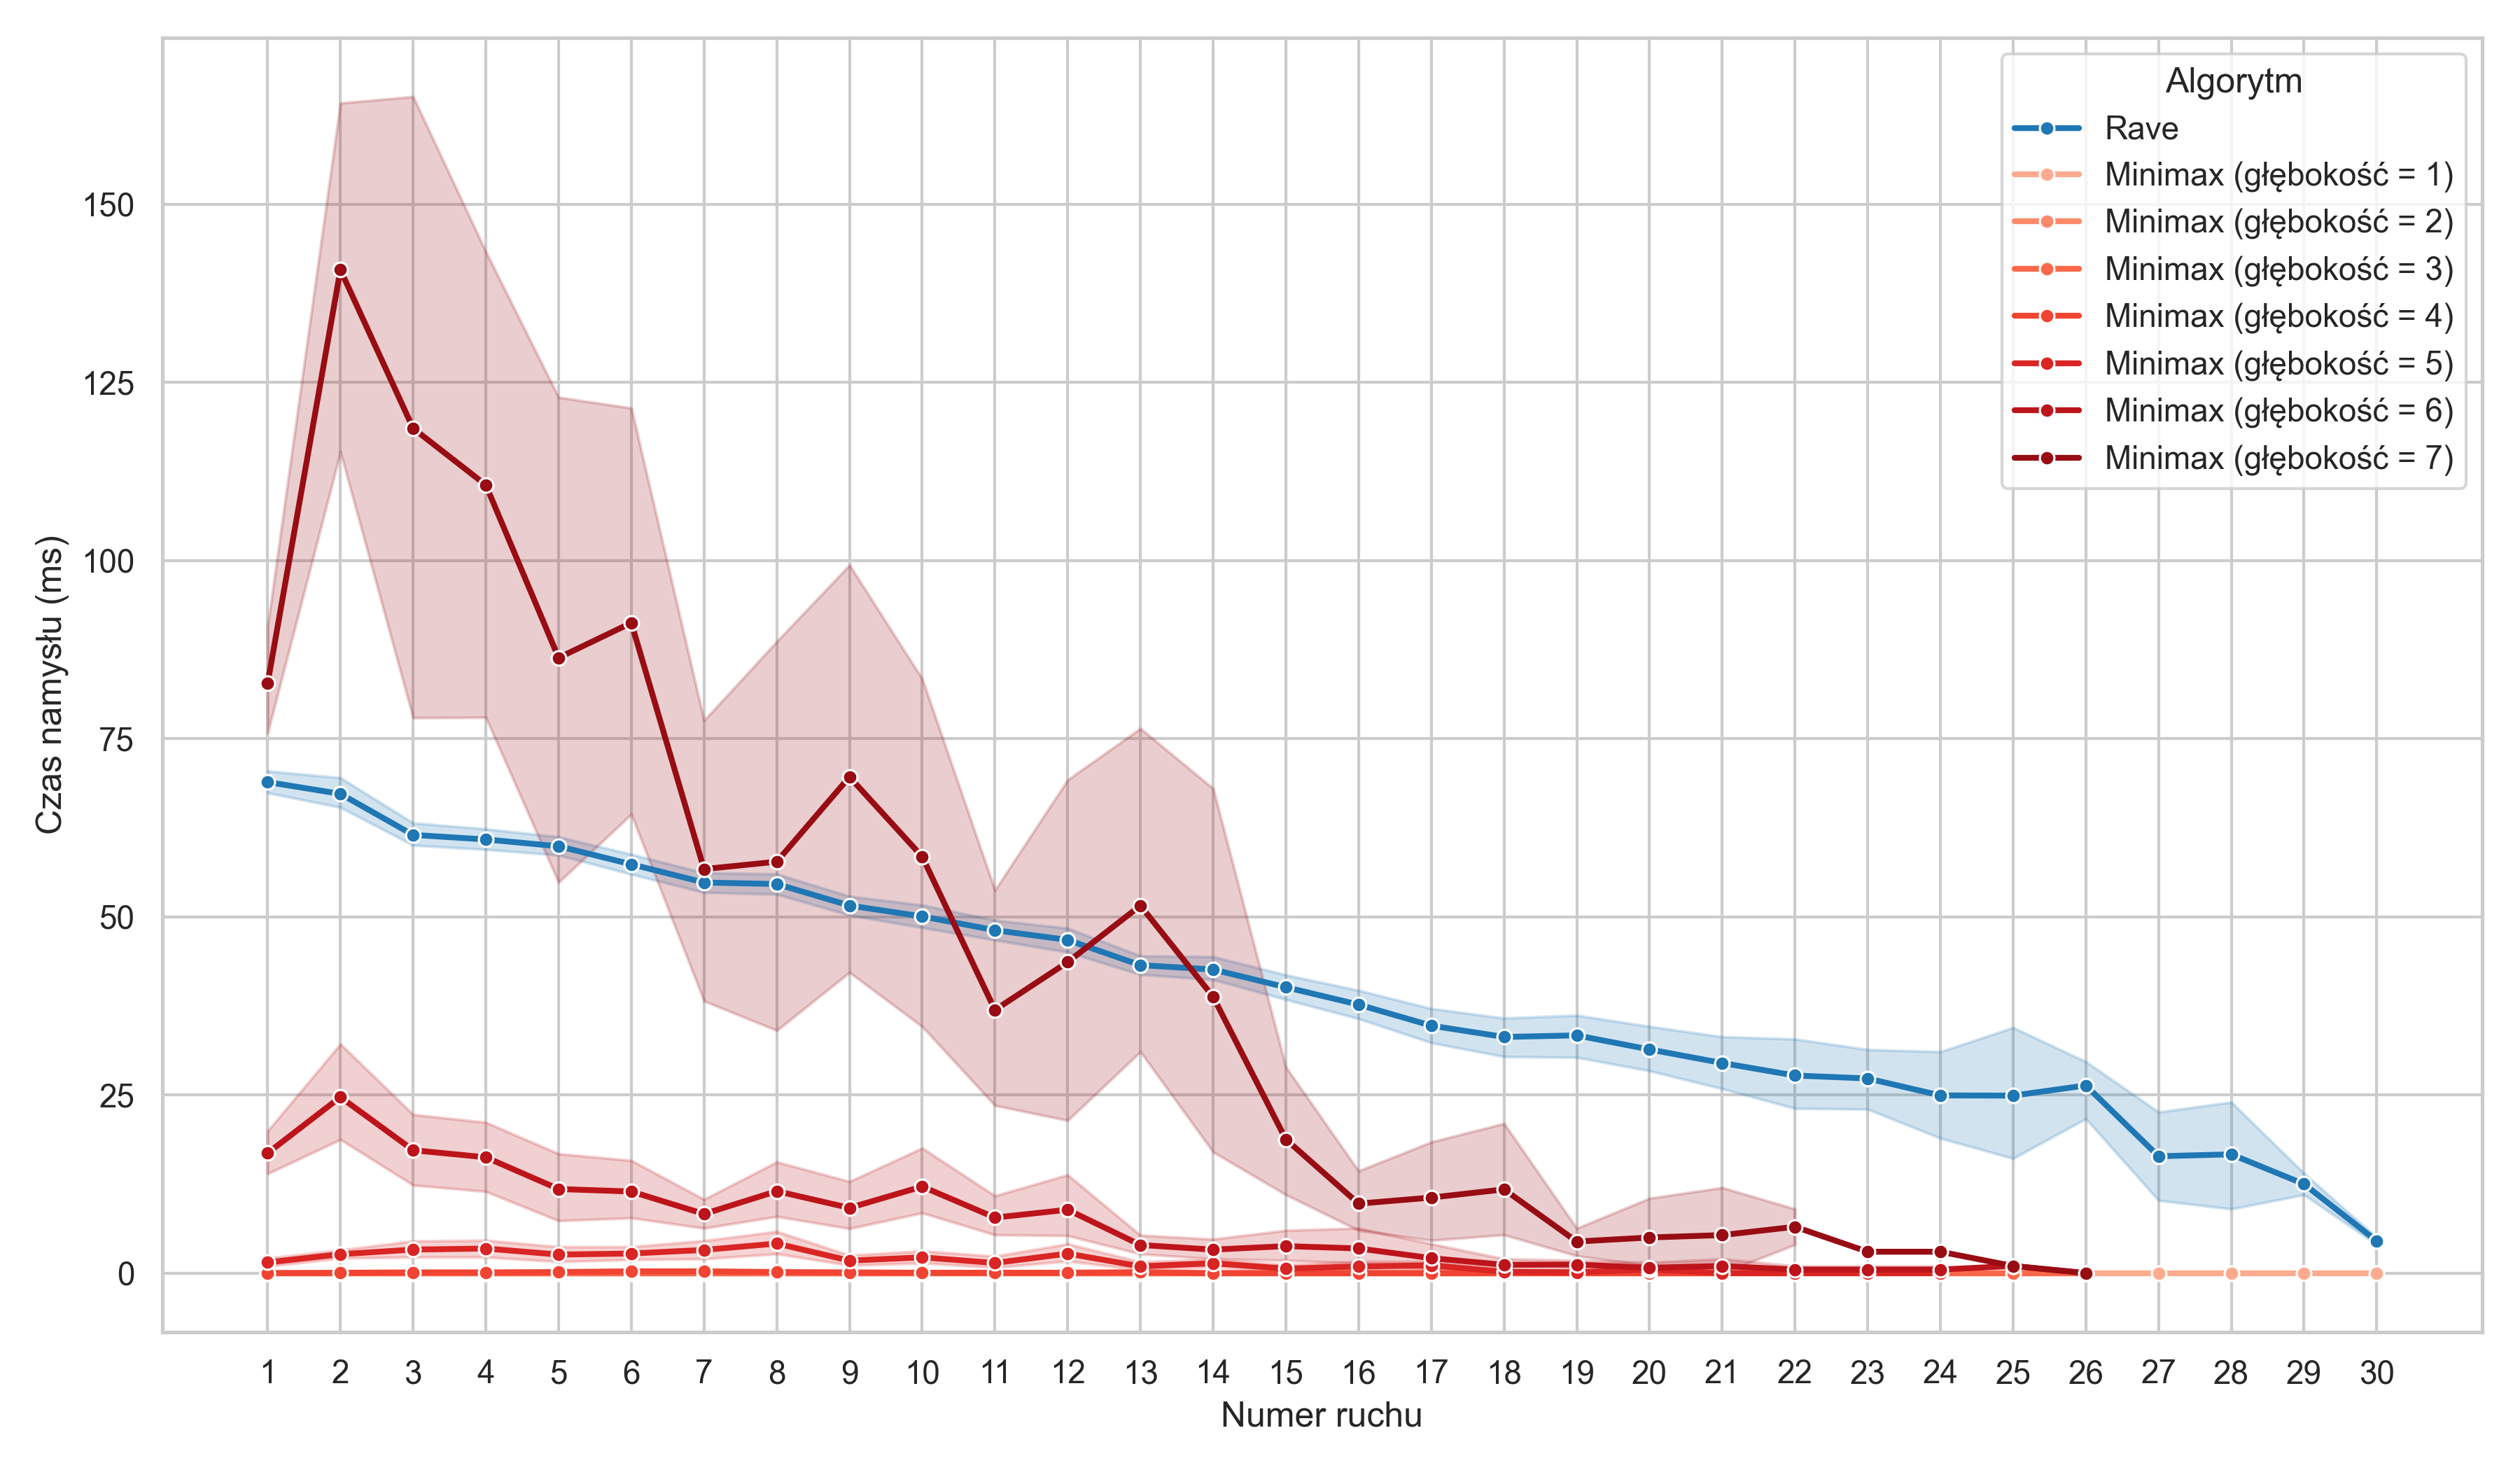
\includegraphics[width=\textwidth]{images/rave_thinking_time.png}
        \caption{MCTS + RAVE}
        \label{fig:time-rave}
    \end{subfigure}

    \vspace{0.5cm}

    \begin{subfigure}[b]{0.49\textwidth}
        \centering
        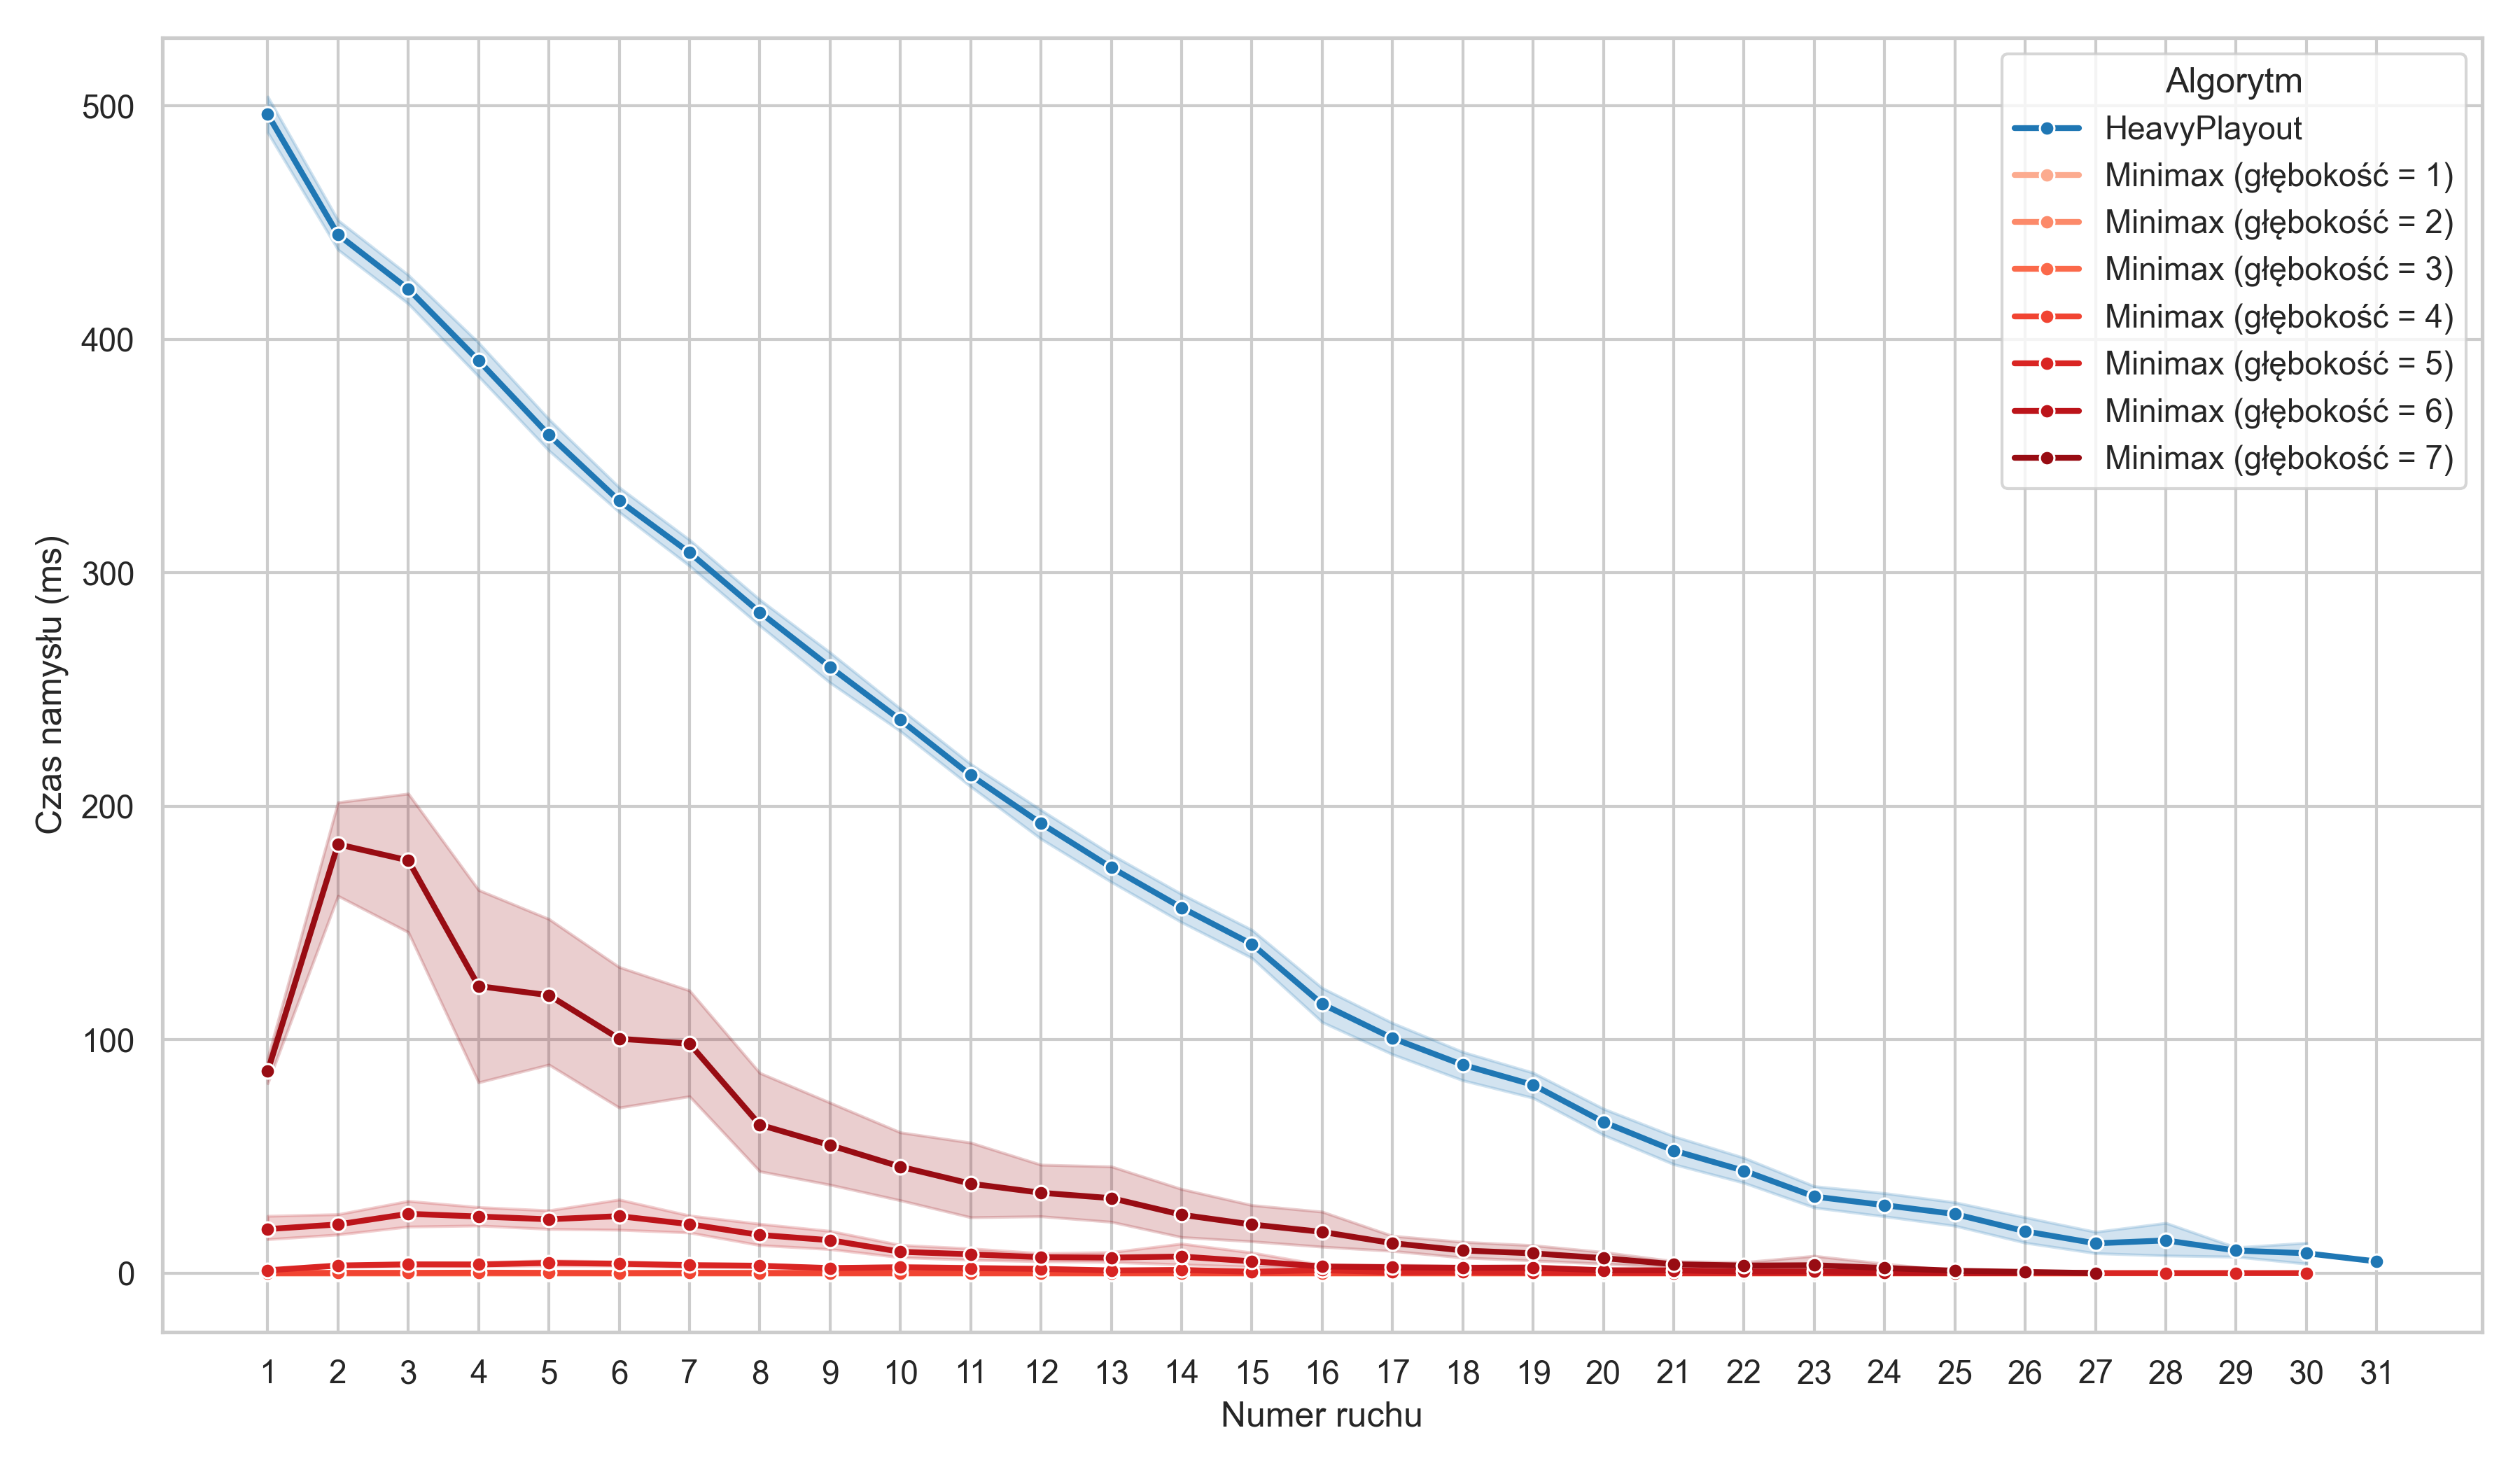
\includegraphics[width=\textwidth]{images/heavyplayouts_thinking_time.png}
        \caption{MCTS + Heavy Playouts}
        \label{fig:time-heavy}
    \end{subfigure}

    \caption{Średni czas namysłu (w milisekundach) dla różnych wariantów algorytmu MCTS oraz ich przeciwników (agenta Minimax o rosnącej głębokości przeszukiwania).}
    \label{fig:comparison-time}
\end{figure}

\noindent
Ostatnim, w ramach tego eksperymentu, badanym elementem była analiza średniego czasu namysłu wymaganego do wygenerowania pojedynczego ruchu. Profile wydajnościowe, zestawione na układzie wykresów (Rysunek~\ref{fig:comparison-time}), obrazują różnice w naturze obu podejść do przeszukiwania przestrzeni stanów.

Przewidywalną obserwacją, jest wykładniczy wzrost czasu namysłu algorytmu Minimax wraz ze wzrostem limitu głębokości przeszukiwania ($d$). Dla płytkich wartości ($d \le 4$), decyzje podejmowane są niemal natychmiastowo, jednakże przekroczenie progu $d=5$ powoduje drastyczne wzrost wielkości drzewa gry (wynikające z wysokiego współczynnika rozgałęzienia w gry). Dla maksymalnej testowanej głębokości ($d=7$), pojedynczy ruch oponenta statycznego zajmuje znacząco więcej czasu niż iteracyjne rozwijanie drzewa przez warianty MCTS oraz MCTS + RAVE, co pokazuje ograniczenia skalowalności naiwnego (bądź wyposażonego jedynie w cięcia alfa-beta) przeglądu zupełnego.

Ciekawszym zjawiskiem jest zachowanie czasu namysłu dla algorytmów opartych na MCTS. Mimo iż operowały one na stałym, odgórnie narzuconym limicie całkowitej liczby iteracji w każdym ruchu (niezależnie od przeciwnika), czas potrzebny na realizację tego budżetu skraca się (w przybliżeniu liniowo) wraz z rozwojem gry. Losowe lub pół-losowe rozgrywki algorytmów MCTS trwają coraz krócej ponieważ pozostało niewiele ruchów do zakończenia rozgrywki.

Analizując warianty MCTS między sobą, można zauważyć, że zastosowanie heurystyki RAVE nie wprowadziło znaczącego narzutu obliczeniowego, natomiast wielokrotne wywoływanie funkcji oceny pozycji w wariancie Heavy Playouts, dosyć znacząco wydłuża czas namysłu algorytmu, którego średni czas namysłu do 11 ruchu przekracza 200 ms (przy stałym limicie 10000 iteracji).

\subsubsection{Wnioski końcowe}

Analiza zebranych danych pozwala stwierdzić, że dla najbardziej podstawowego wariantu płytkiego przeszukiwania, czyli dla głębokości $d=1$, wszystkie testowane modyfikacje algorytmu stochastycznego z sukcesem osiągnęły lub przekroczyły wymagany próg skuteczności. Klasyczny wariant MCTS uzyskał wynik 95.0\%, MCTS z heurystyką RAVE osiągnął barierę 70.0\%, natomiast wariant kierowany (Heavy Playouts) zdominował przeciwnika całkowicie, wygrywając 100.0\% rozegranych partii.

\textbf{Hipoteza H3 zostaje przyjęta}. Należy jednak zaznaczyć, że założony próg 70\% wygranych jest spełniony wyłącznie dla głębokości równej 1. Zwiększenie horyzontu planowania agenta Minimax zaledwie o jeden lub dwa półruchy ($d \ge 2$) powodowało gwałtowne załamanie skuteczności metod opartych o algorytm MCTS.

\newpage
\subsection{Hipoteza 4: Wpływ rozmiaru planszy na asymetrię szans}

\subsubsection{Metodologia i przebieg eksperymentu}

Weryfikacja czwartej hipotezy badawczej (H4) koncentrowała się na ocenie wpływu geometrii planszy na asymetrię szans w grze. Ze względu na specyfikę mechaniki Breakthrough, w której celem jest dotarcie do linii końcowej przeciwnika, gracz wykonujący pierwszy ruch (białe) dysponuje naturalną przewagą tempa. Hipoteza zakładała, że wraz ze wzrostem wymiarów planszy przewaga koloru białego ulegnie marginalizacji na rzecz strategii. Zgodnie z hipotezą, zmodyfikowane algorytmy MCTS będą w stanie odnosić relatywnie częstsze zwycięstwa z pozycji czarnych na większych planszach.

Rozgrywki przeprowadzono dla asymetrycznych wymiarów planszy. Szerokość ustalono jako stałą wartość $W = 8$, natomiast wysokość ($H$) stanowiła zmienną niezależną przyjmującą wartości z rosnącego zbioru: $H \in \{5, 6, 7, 8, 9, 10, 11\}$. 

Eksperyment podzielono na trzy symetryczne serie pomiarowe, w których po obu stronach planszy stawali identyczni agenci:
\begin{enumerate}
    \item \textbf{Seria 1:} Klasyczny algorytm MCTS (UCT) grający przeciwko sobie.
    \item \textbf{Seria 2:} Wariant MCTS + RAVE.
    \item \textbf{Seria 3:} Wariant MCTS + Heavy Playouts.
\end{enumerate}

\noindent
Aby zapewnić agentom budżet adekwatny do rozmiaru gry, maksymalna liczba iteracji zmieniała się liniowo w zależności od wysokości planszy zgodnie ze wzorem:

$$I = 2000 \cdot H$$

\noindent
Tym samym dla planszy $8 \times 5$ limit wynosił 10000 iteracji, a dla $8 \times 11$ już 22000. \\

\noindent
Dla każdego z testowanych wymiarów planszy i dla każdej z trzech serii rozegrano dokładnie 50 partii turniejowych. Ponieważ w każdej serii agenci reprezentowali identyczną siłę gry, zrezygnowano z rotacji kolorów na rzecz jednorodnego monitorowania współczynnika zwycięstw z perspektywy białego gracza.

\subsubsection{Analiza wyników}

Zgromadzone dane pozwoliły na prześledzenie zachowania wskaźnika zwycięstw dla gracza rozpoczynającego (Białe) w zależności od wysokości planszy $H$. Zestawienie wyników dla wszystkich trzech symetrycznych par algorytmów (Klasyczny MCTS, MCTS + RAVE, MCTS + Heavy Playouts) przedstawiono w formie wykresów na Rysunku~\ref{fig:h4-winrate-comparison}. Szczegółowe dane liczbowe zostały zgromadzone w Tabeli~\ref{tab:h4-summary}.

\begin{figure}[H]
    \centering

    \begin{subfigure}[b]{0.49\textwidth}
        \centering
        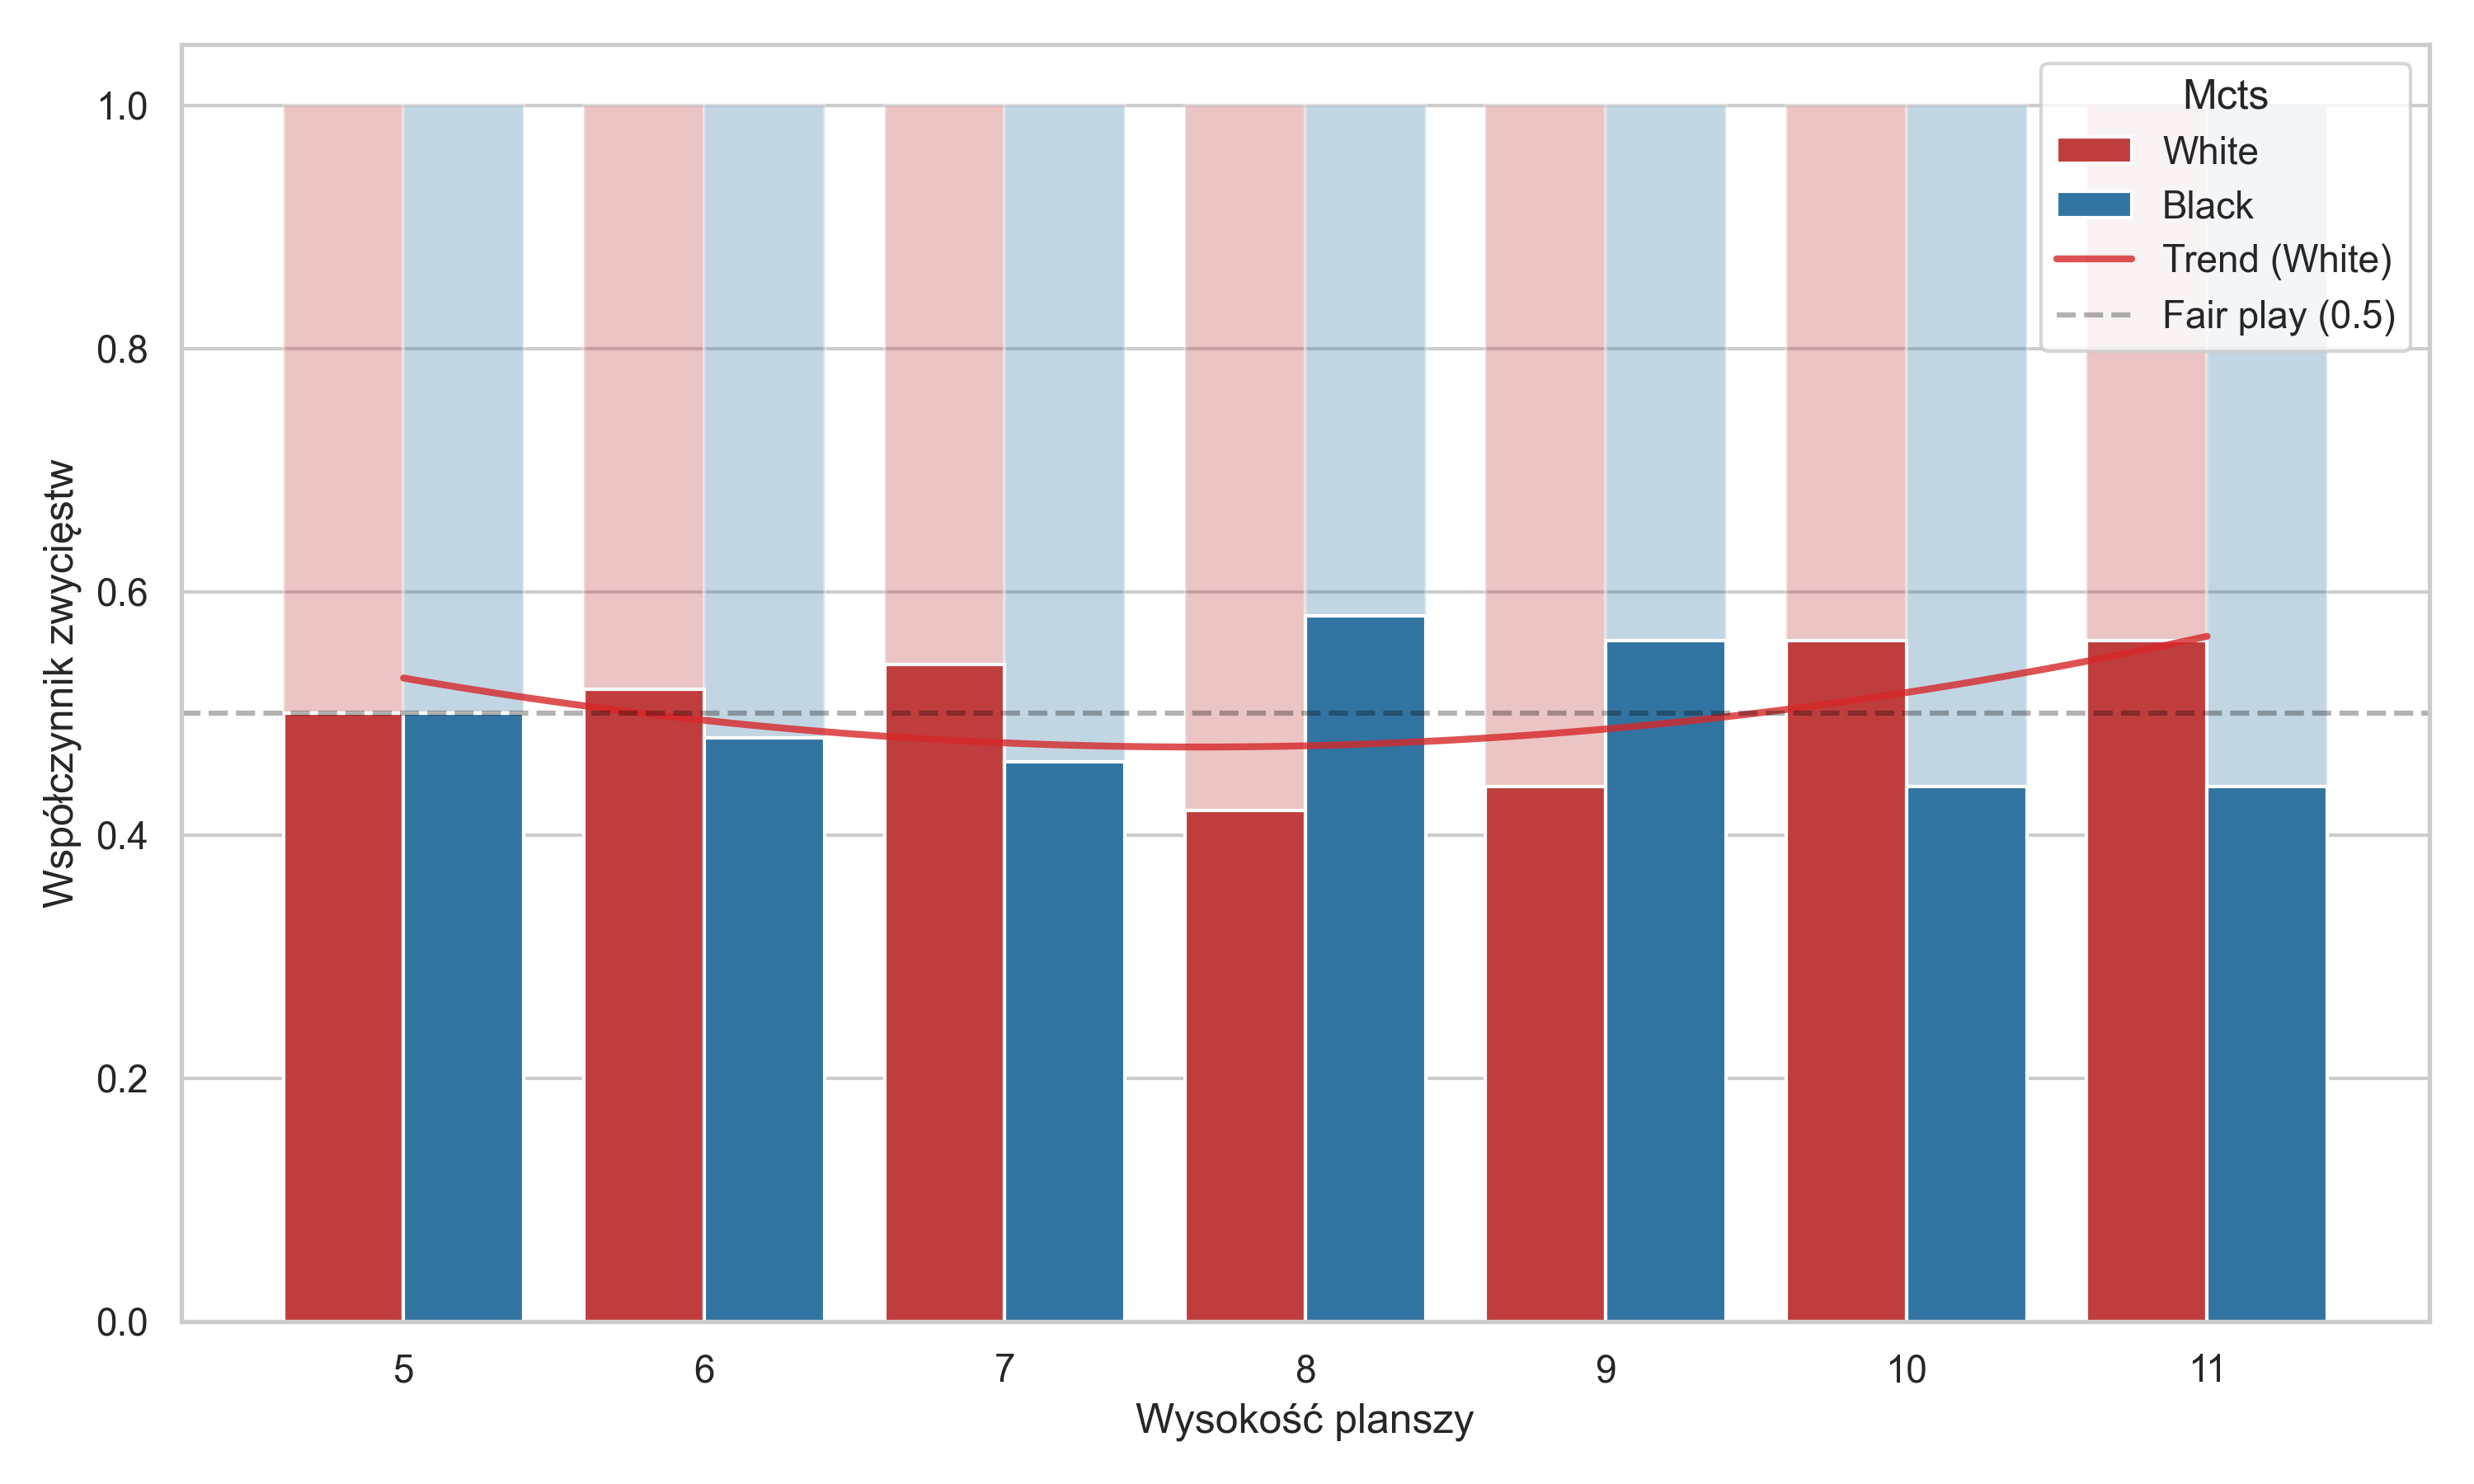
\includegraphics[width=\textwidth]{images/mcts_board_size_win_rate.png}
        \caption{Klasyczny MCTS}
        \label{fig:h4-mcts}
    \end{subfigure}
    \hfill
    \begin{subfigure}[b]{0.49\textwidth}
        \centering
        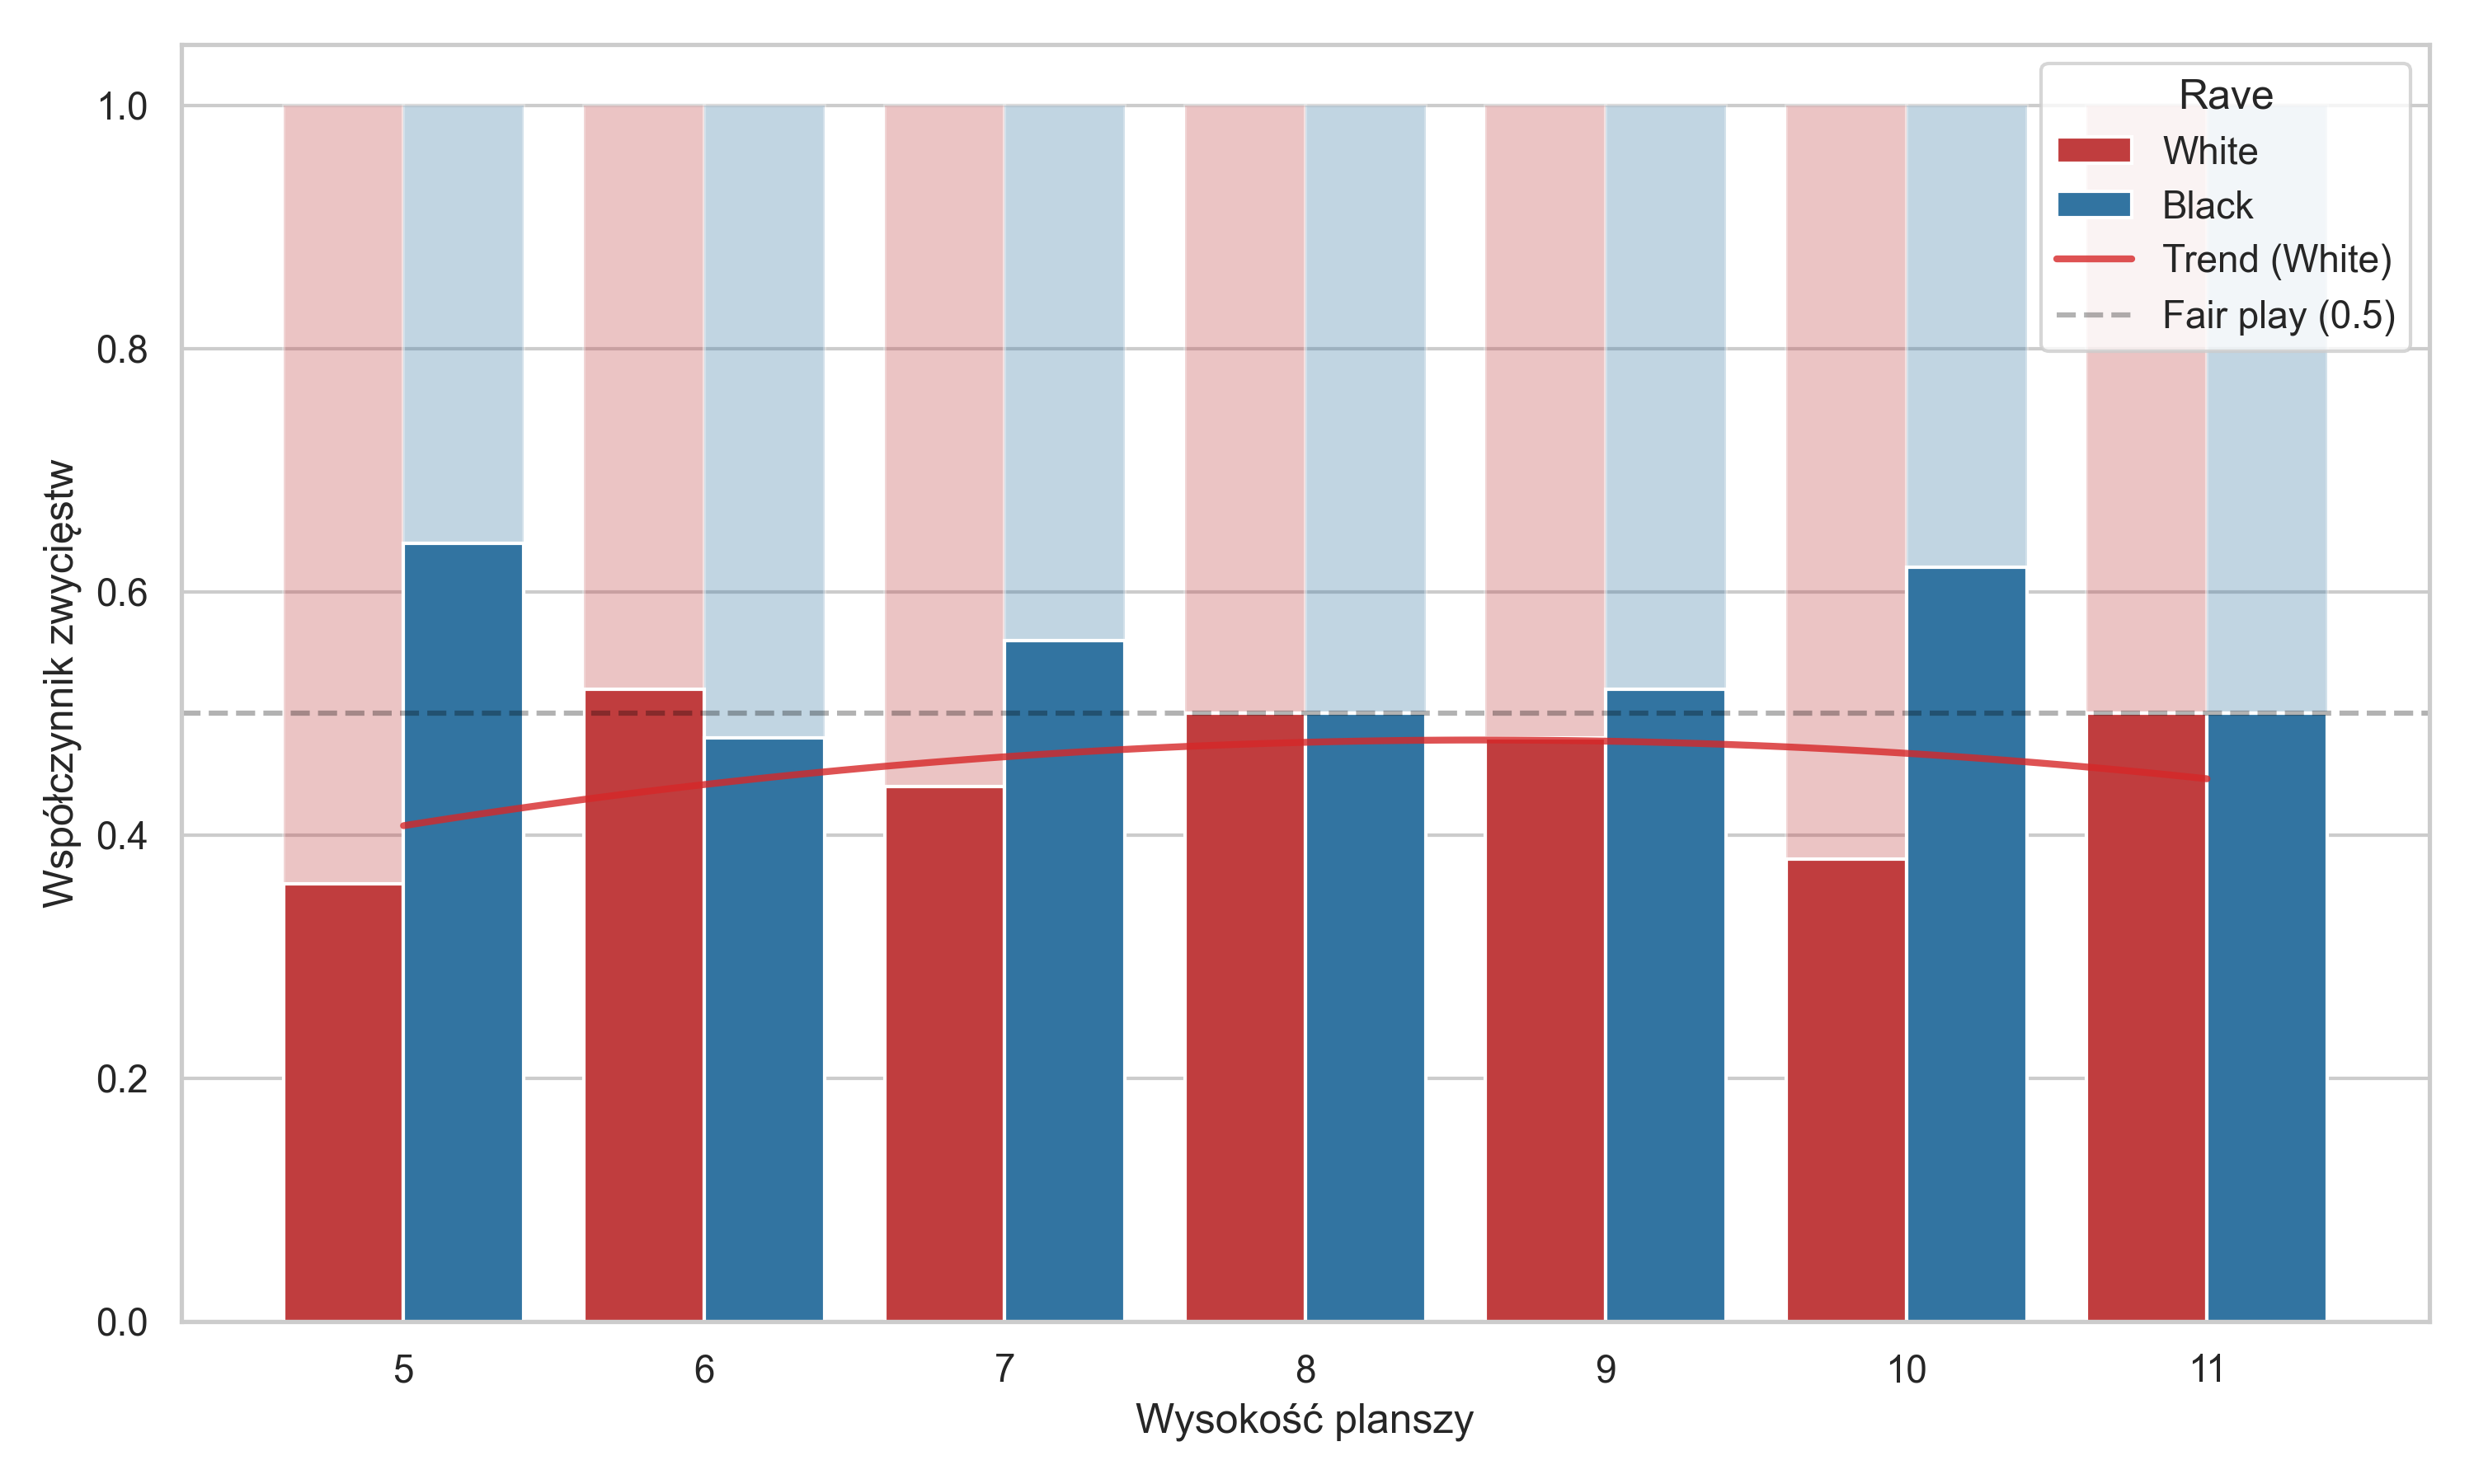
\includegraphics[width=\textwidth]{images/rave_board_size_win_rate.png}
        \caption{MCTS + RAVE}
        \label{fig:h4-rave}
    \end{subfigure}

    \vspace{0.5cm}

    \begin{subfigure}[b]{0.49\textwidth}
        \centering
        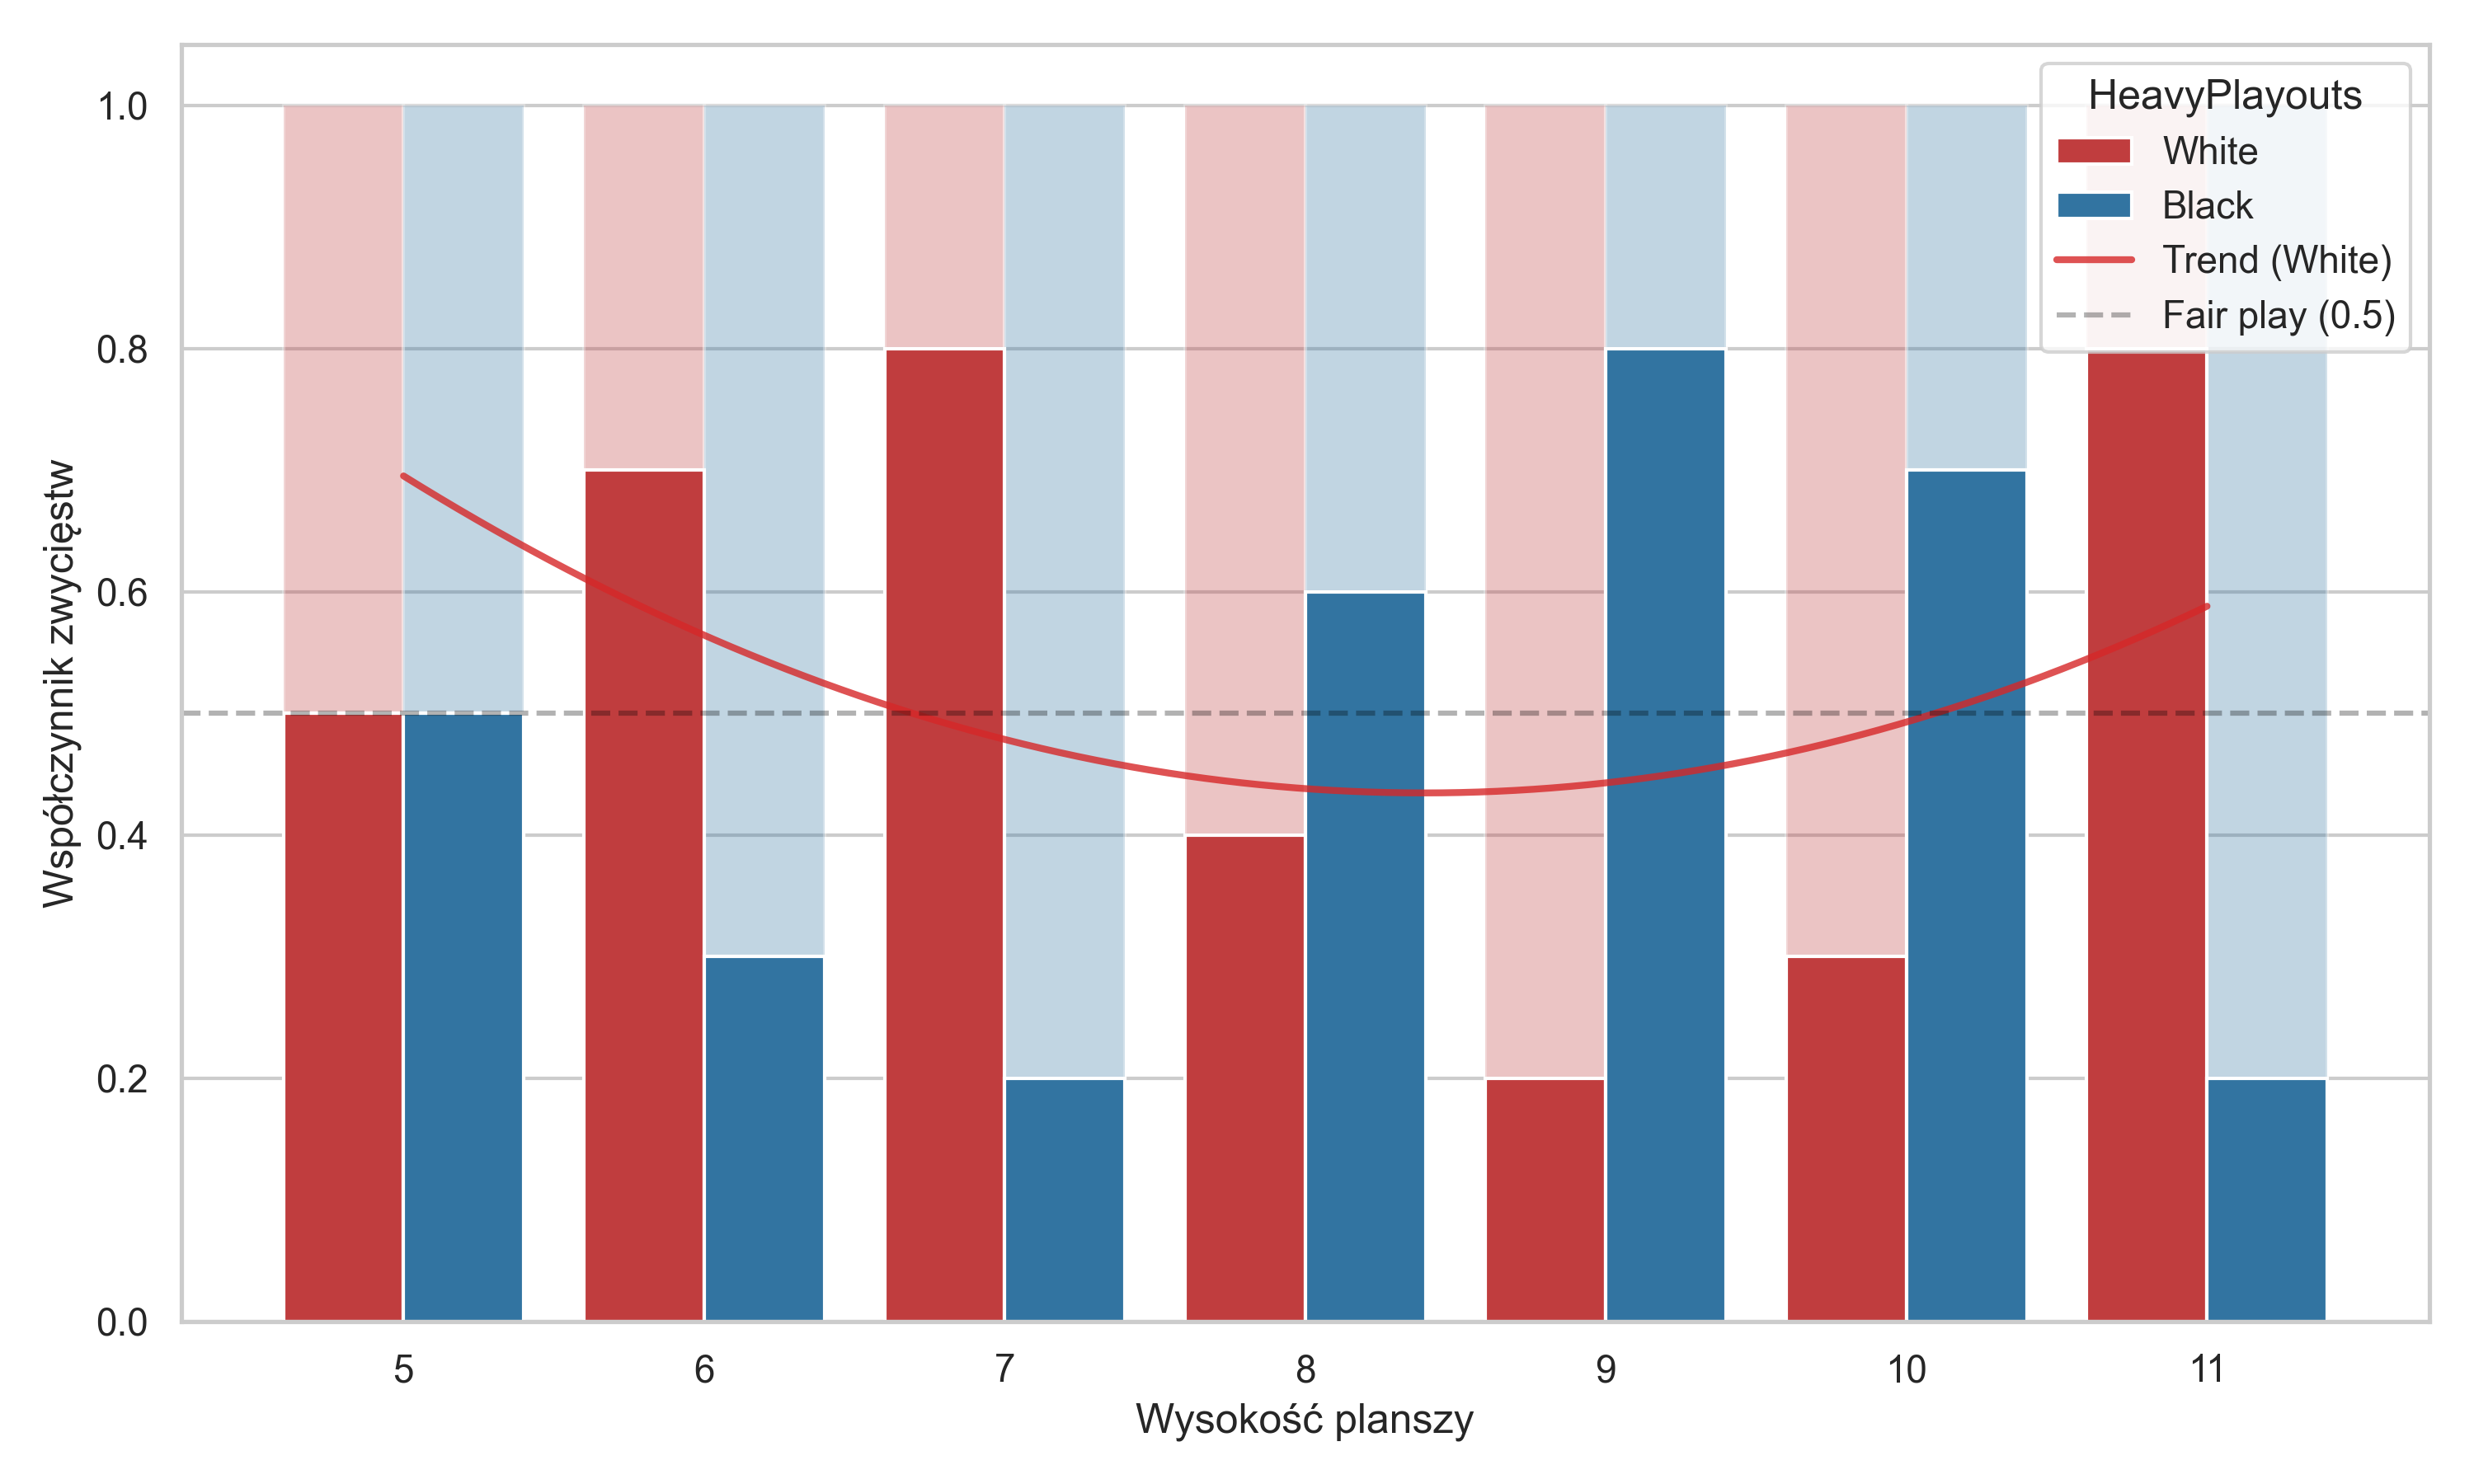
\includegraphics[width=\textwidth]{images/heavyplayouts_board_size_win_rate.png}
        \caption{MCTS + Heavy Playouts}
        \label{fig:h4-heavy}
    \end{subfigure}

    \caption{Odsetek zwycięstw gracza rozpoczynającego (Białe) w starciach symetrycznych w zależności od wysokości planszy ($H$) przy stałej szerokości $W=8$.}
    \label{fig:h4-winrate-comparison}
\end{figure}

\noindent
Wstępna analiza wyników wskazuje na dużą zmienność (wariancję) wskaźnika wygranych w poszczególnych wariantach na szerokim przedziale wysokości planszy. W celu ułatwienia interpretacji tych odchyleń, na wykresach naniesiono linię trendu obrazującą ogólną tendencję zmian skuteczności (modelowaną przez wielomian stopnia 2), a także poziomą linię wyznaczającą próg 50\% (tzw. linię \textit{fair play}), która reprezentuje stan idealnej równowagi szans między stroną rozpoczynającą a broniącą.

Analiza zgromadzonych danych pozwala na pozytywne zweryfikowanie postawionych warunków. Rozpatrując kluczowy przedział wysokości od $H=7$ do $H=9$, zaobserwowano spadek odsetka wygranych Białego. Dla klasycznego MCTS skuteczność Białych spadła z poziomu 54.0\% ($H=7$) do 42.0\% ($H=8$) oraz 44.0\% ($H=9$), co oznacza utratę inicjatywy startowej i przejście inicjatywy (choć z niewielką przewagą) na stronę Czarnych.

Wprowadzenie wiedzy domenowej poprzez modyfikację Heavy Playouts ujawniło wyraźny trend malejący: od dominacji Białych wynoszącej 80.0\% na planszy $8 \times 7$, poprzez spadek do 40.0\% na planszy $8 \times 8$, aż do zaledwie 20.0\% na planszy $8 \times 9$.

Należy zaznaczyć, że trend ten nie zachowuje idealnej liniowości w nieskończoność (co pokazują anomalie dla dużej planszy $H=11$), a wariant RAVE charakteryzował się większą zachowawczością wyników wokół linii remisu (50\%). Nie zmienia to jednak faktu, że w zakładanym w kryteriach przedziale badawczym (odpowiednik plansz średnich i dużych) zjawisko marginalizacji przewagi Białych jest zauważalne.

\begin{table}[H]
    \centering
    \caption{Zestawienie skuteczności i średniej długości partii dla wariantów MCTS w zależności od wysokości planszy.}
    \label{tab:h4-summary}
    \renewcommand{\arraystretch}{1.2}

    \begin{tabular}{|p{1.5cm}|p{1.8cm}|p{2.7cm}|p{2.1cm}|}
        \hline
        \textbf{Wariant} & \textbf{Wysokość planszy} & \textbf{Współczynnik zwycięstw (Białe/Czarne)} & \textbf{Średnia długość partii} \\
        \hline

        \multirow{7}{1.5cm}{Klasyczny MCTS}
            & \hfill 5  & \hfill 50/50\% & \hfill 15.8 $\pm$ 3.5 \\
            & \hfill 6  & \hfill 52/48\% & \hfill 20.4 $\pm$ 4.1 \\
            & \hfill 7  & \hfill 54/46\% & \hfill 25.4 $\pm$ 6.2 \\
            & \hfill 8  & \hfill 42/58\% & \hfill 29.1 $\pm$ 7.7 \\
            & \hfill 9  & \hfill 44/56\% & \hfill 31.3 $\pm$ 7.2 \\
            & \hfill 10 & \hfill 56/44\% & \hfill 39.2 $\pm$ 8.4 \\
            & \hfill 11 & \hfill 56/44\% & \hfill 38.5 $\pm$ 10.7 \\
        \hline
        
        \multirow{7}{1.5cm}{MCTS + Heavy Playouts}
            & \hfill 5  & \hfill 50/50\% & \hfill 16.3 $\pm$ 1.7 \\
            & \hfill 6  & \hfill 70/30\% & \hfill 19.8 $\pm$ 4.7 \\
            & \hfill 7  & \hfill 80/20\% & \hfill 27.5 $\pm$ 2.6 \\
            & \hfill 8  & \hfill 40/60\% & \hfill 34.9 $\pm$ 5.1 \\
            & \hfill 9  & \hfill 20/80\% & \hfill 40.7 $\pm$ 4.0 \\
            & \hfill 10 & \hfill 30/70\% & \hfill 52.7 $\pm$ 6.4 \\
            & \hfill 11 & \hfill 80/20\% & \hfill 56.5 $\pm$ 3.8 \\
        \hline


        \multirow{7}{1.5cm}{MCTS + RAVE}
            & \hfill 5  & \hfill 36/64\% & \hfill 15.2 $\pm$ 3.2 \\
            & \hfill 6  & \hfill 52/48\% & \hfill 18.4 $\pm$ 4.1 \\
            & \hfill 7  & \hfill 44/56\% & \hfill 19.7 $\pm$ 4.3 \\
            & \hfill 8  & \hfill 50/50\% & \hfill 23.0 $\pm$ 5.2 \\
            & \hfill 9  & \hfill 48/52\% & \hfill 25.6 $\pm$ 5.9 \\
            & \hfill 10 & \hfill 38/62\% & \hfill 28.6 $\pm$ 7.0 \\
            & \hfill 11 & \hfill 50/50\% & \hfill 30.9 $\pm$ 8.5 \\
        \hline

    \end{tabular}
\end{table}

\subsubsection{Wnioski końcowe}

\textbf{Hipoteza 4 zostaje przyjęta}. Rozmiar planszy w grze Breakthrough w istotne znaczenie na balans rozgrywki, a na rozszerzonych planszach przemyślana strategia (reprezentowana przez ukierunkowane symulacje) pozwala na statystycznie istotne przejęcie kontroli nad partią przez gracza broniącego (Czarne).

\newpage
\section{Testy z udziałem ludzi}

\subsection{Metodologia i przebieg badania}

Ostatnim etapem ewaluacji była seria rozgrywek z udziałem ludzi. Celem tego eksperymentu była analiza tego, jak agent radzi sobie z przeciwnikiem, który nie gra według deterministycznego skryptu, może świadomie wykorzystywać słabości zauważone w trakcie rozgrywki oraz adaptować się do stylu gry przeciwnika.

W badaniu wzięło udział pięciu testerów, którzy nie byli twórcami agentów. Każdy z nich rozegrał osiem partii: po jednej przeciwko każdemu z agentów na planszy $7 \times 7$ oraz po jednej na planszy $8 \times 8$. Łącznie zebrano więc 40 próbek. Algorytmy były następujące:

\begin{enumerate}
    \item klasyczny MCTS,
    \item MCTS z heurystyką RAVE ze stałą $k=100$,
    \item MCTS z Heavy Playouts,
    \item Minimax o głębokości przeszukiwania $d=8$.
\end{enumerate}

\noindent
W rozgrywkach na planszy $7 \times 7$ człowiek grał kolorem białym, a na planszy $8 \times 8$ kolorem czarnym. Kolejność konfiguracji była zapisana osobno dla każdego uczestnika w plikach \texttt{pXX\_order.csv}. Na końcu każdej rozgrywki uczestnicy badania otrzymywali dwa pytania: o poziom trudności oraz o naturalność strategii przeciwnika i oceniali je w skali od 1 do 5.

\subsection{Analiza wyników}

Zestawienie wyników ilościowych przedstawiono na Rysunkach~\ref{fig:human-winrate-agent}--\ref{fig:human-pieces}. W całym badaniu gracze ludzcy wygrali 27 z 40 rozegranych partii, co odpowiada skuteczności 67.5\%.

\begin{figure}[H]
    \centering
    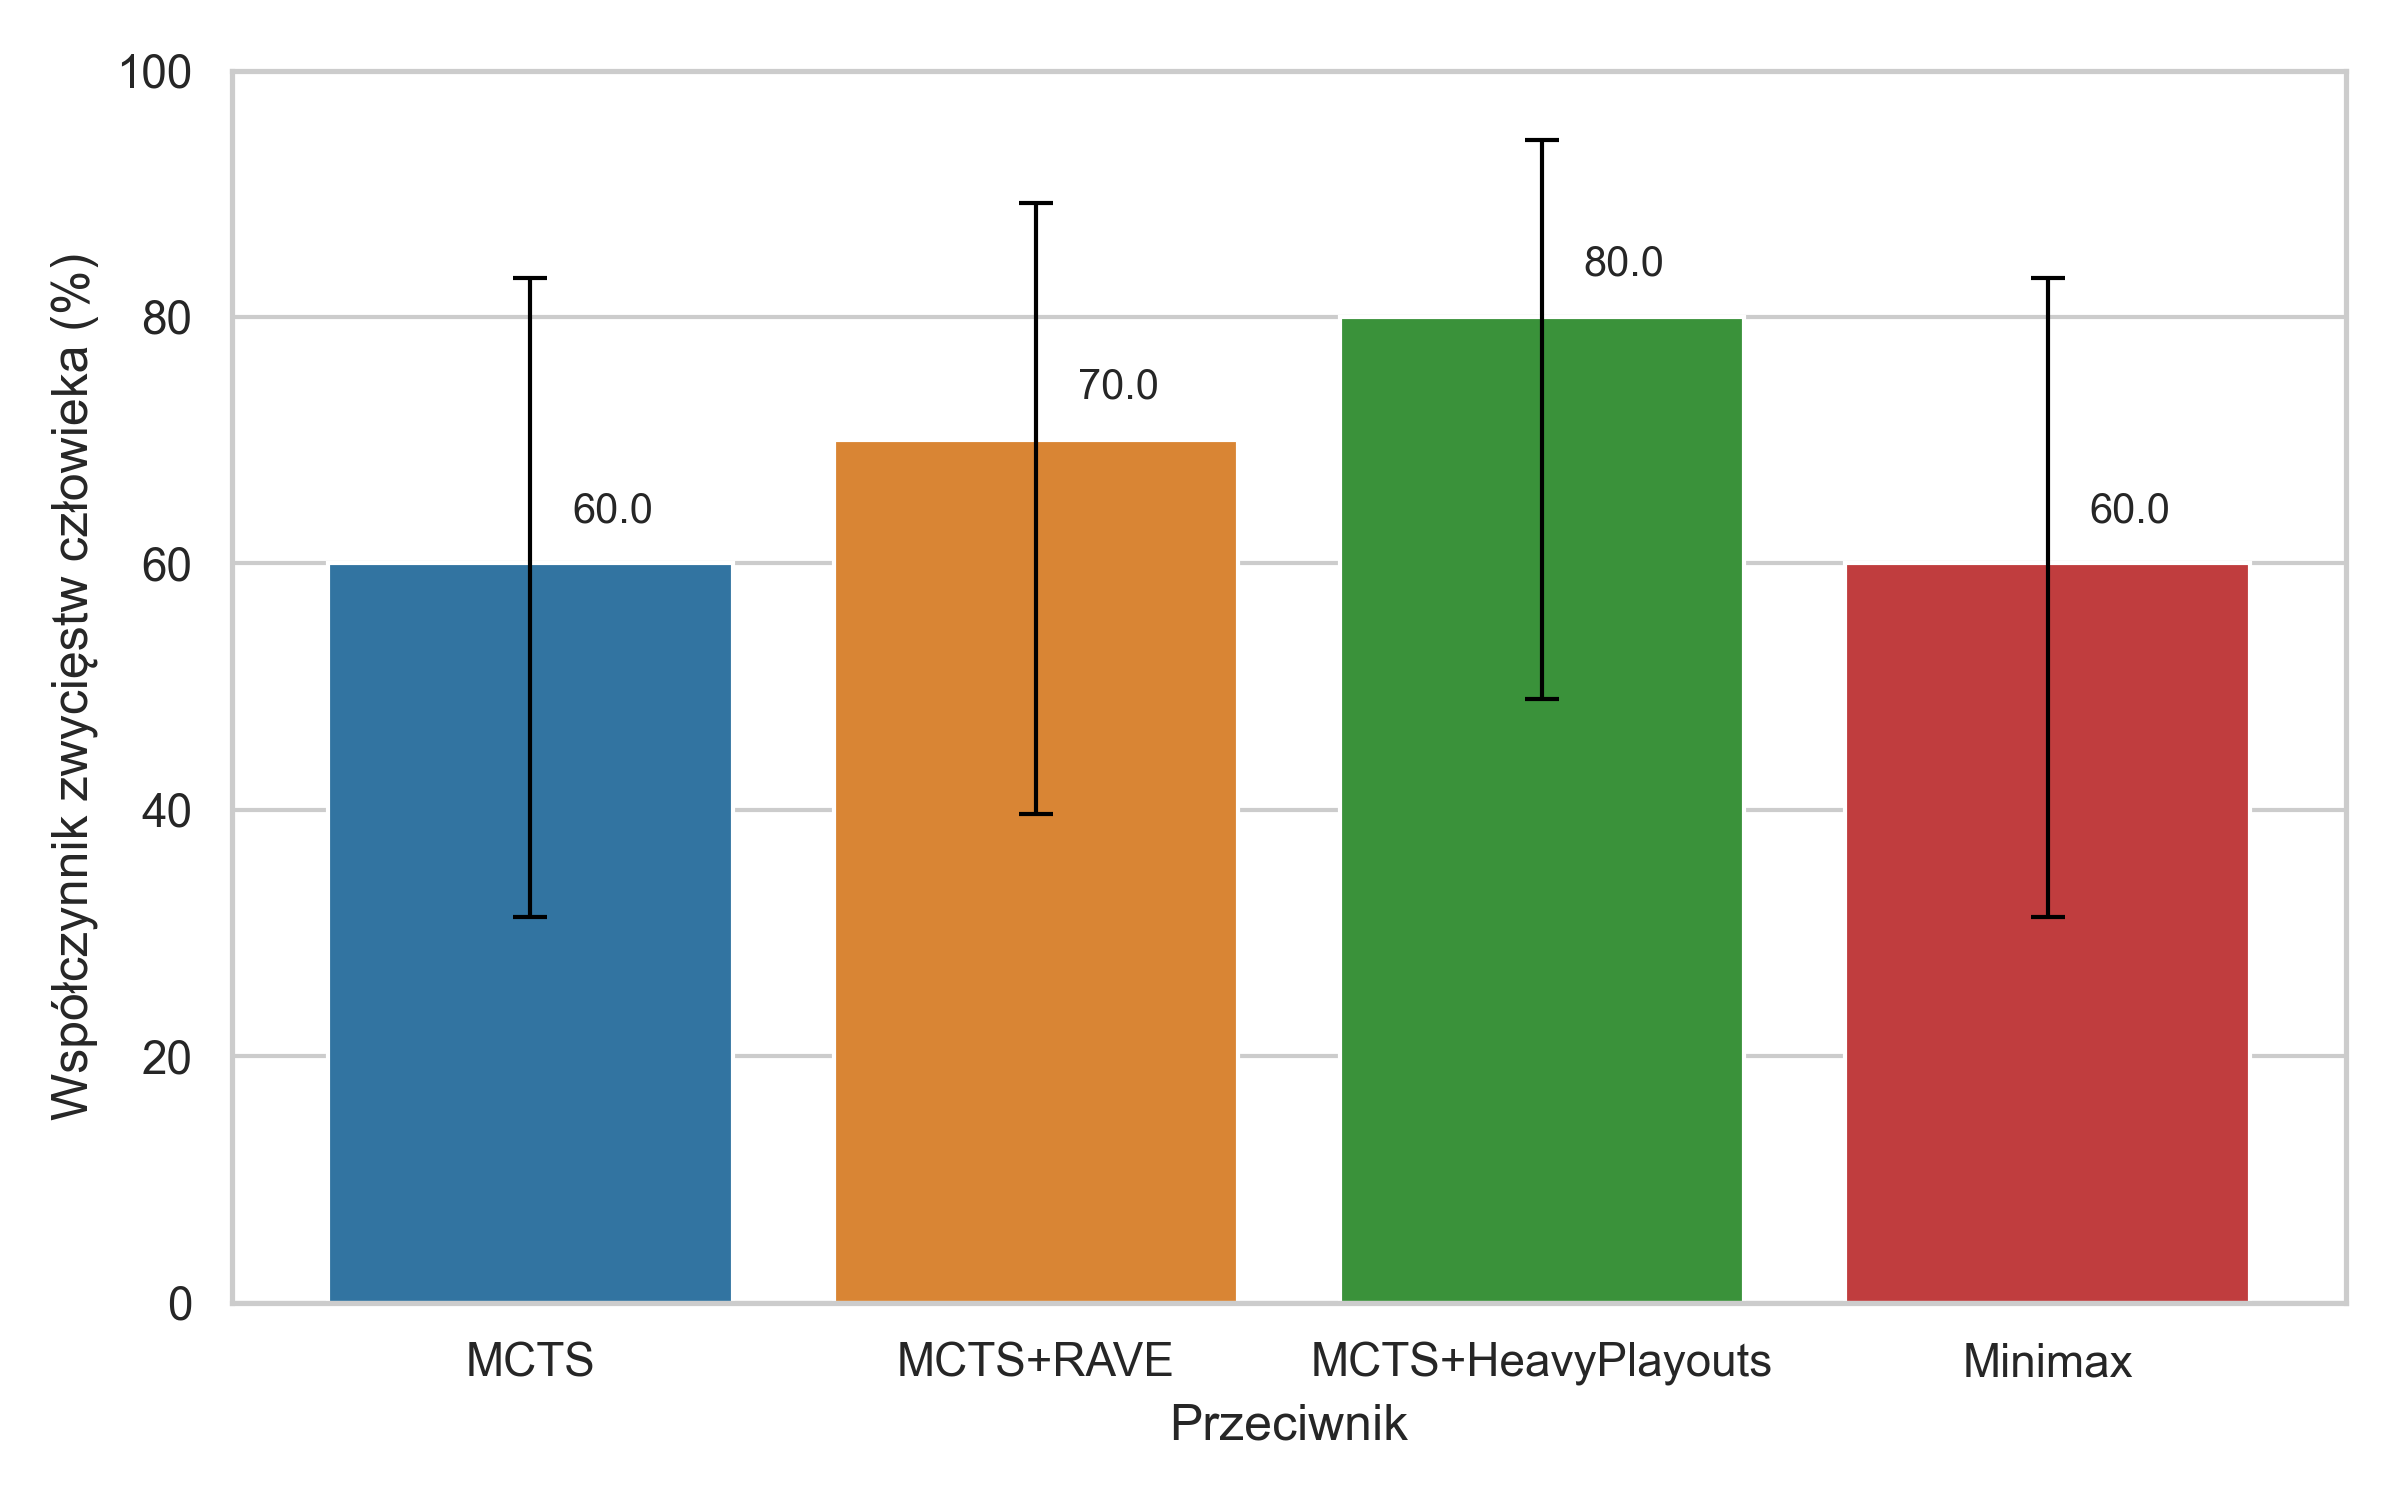
\includegraphics[width=0.78\textwidth]{images/human_win_rate_by_agent.png}
    \caption{Współczynnik zwycięstw ludzi w zależności od wariantu przeciwnika. Słupki błędu oznaczają przedziały ufności Wilsona.}
    \label{fig:human-winrate-agent}
\end{figure}

\noindent
Najwięcej problemów ludziom sprawiały klasyczny MCTS oraz Minimax, przeciwko którym gracze uzyskali po 60.0\% zwycięstw. Najłatwiejszym wariantem w bezpośredniej rywalizacji z ludźmi okazał się MCTS + Heavy Playouts. Testerzy wygrali z nim aż 80.0\% partii.

\begin{figure}[H]
    \centering
    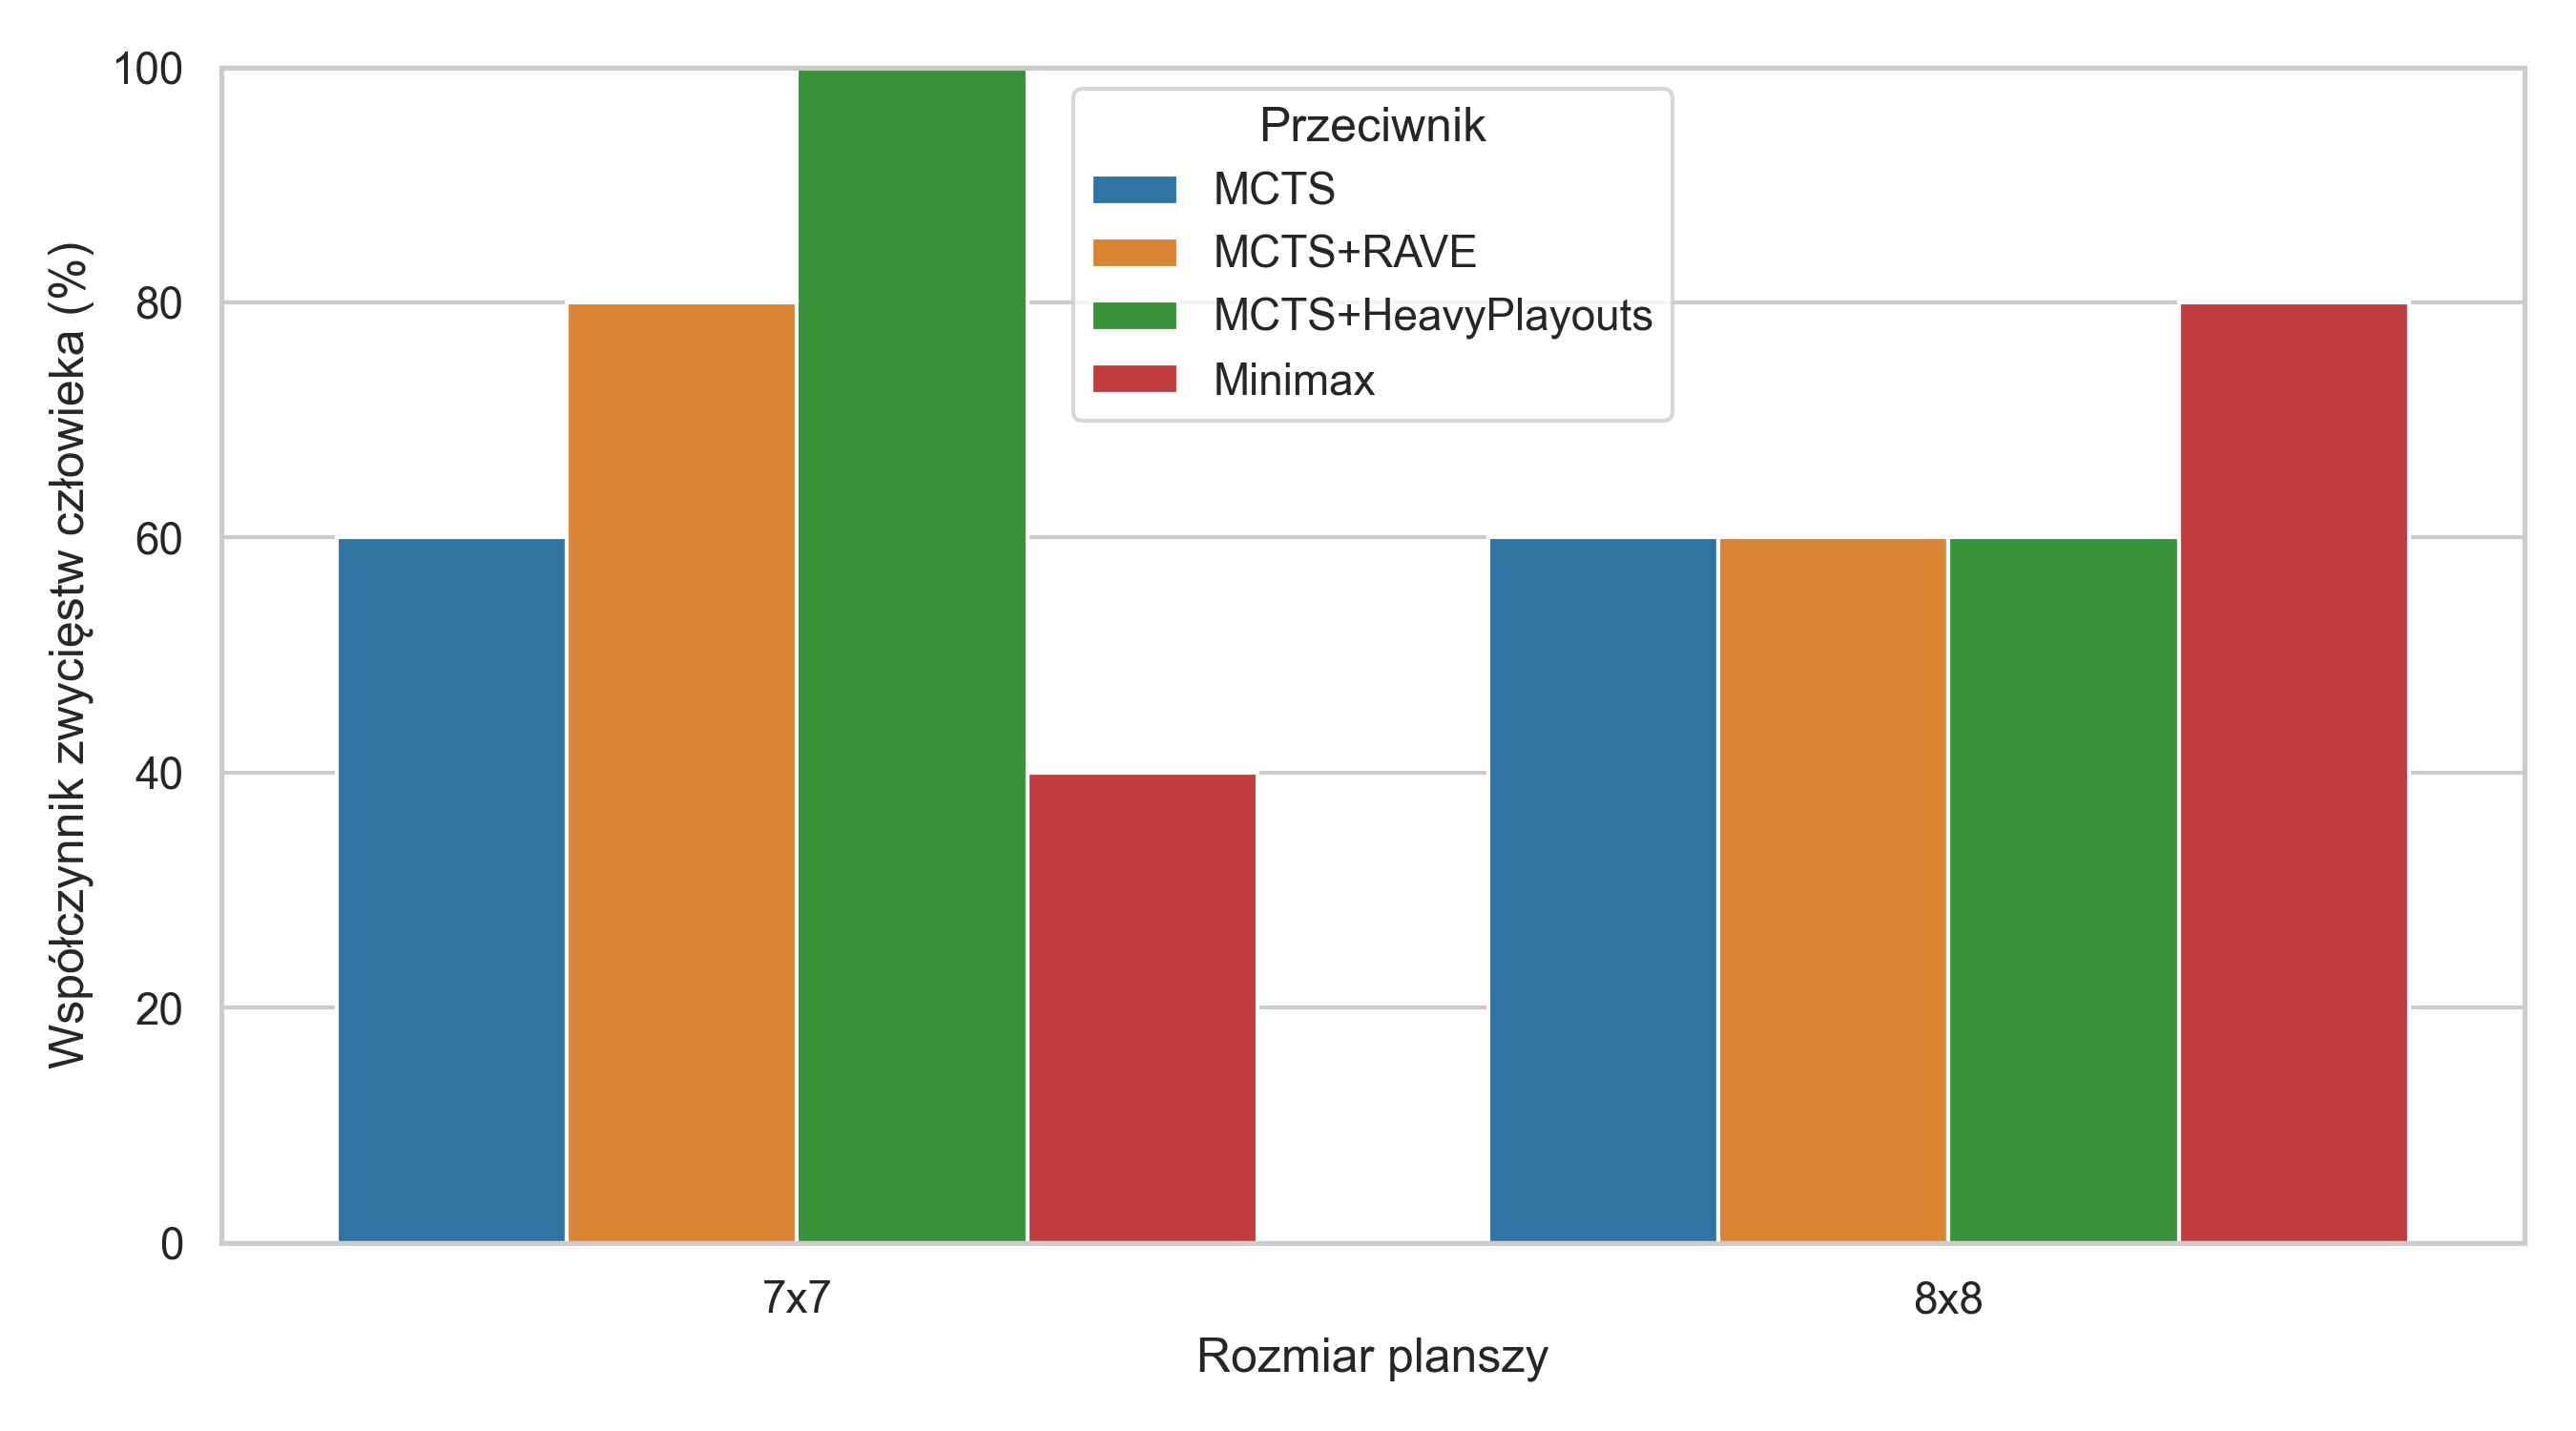
\includegraphics[width=0.82\textwidth]{images/human_win_rate_by_board_and_agent.png}
    \caption{Współczynnik zwycięstw ludzi w podziale na rozmiar planszy oraz wariant przeciwnika.}
    \label{fig:human-winrate-board}
\end{figure}

\noindent
Podział względem rozmiaru planszy wskazuje, że ludzie wygrali 14 z 20 partii na planszy $7 \times 7$ oraz 13 z 20 partii na planszy $8 \times 8$. Oznacza to, że zmiana strony i rozmiaru planszy nie wpłynęła znacząco na sam wynik rozgrywki. Różnice były natomiast widoczne dla konkretnych agentów. Na planszy $7 \times 7$ Minimax wygrał z ludźmi 3 z 5 partii, natomiast na planszy $8 \times 8$ ludzie pokonali go w 4 z 5 partii. Może to sugerować, że na małej planszy taktyczny charakter Minimaxa był trudniejszy do zatrzymania: agent znajdował ścieżki prowadzące piony do celu, które umykały badanym. Na większej planszy gracze mieli więcej przestrzeni do formowania struktur oraz lepszego zarządzania pionami.

\begin{figure}[H]
    \centering
    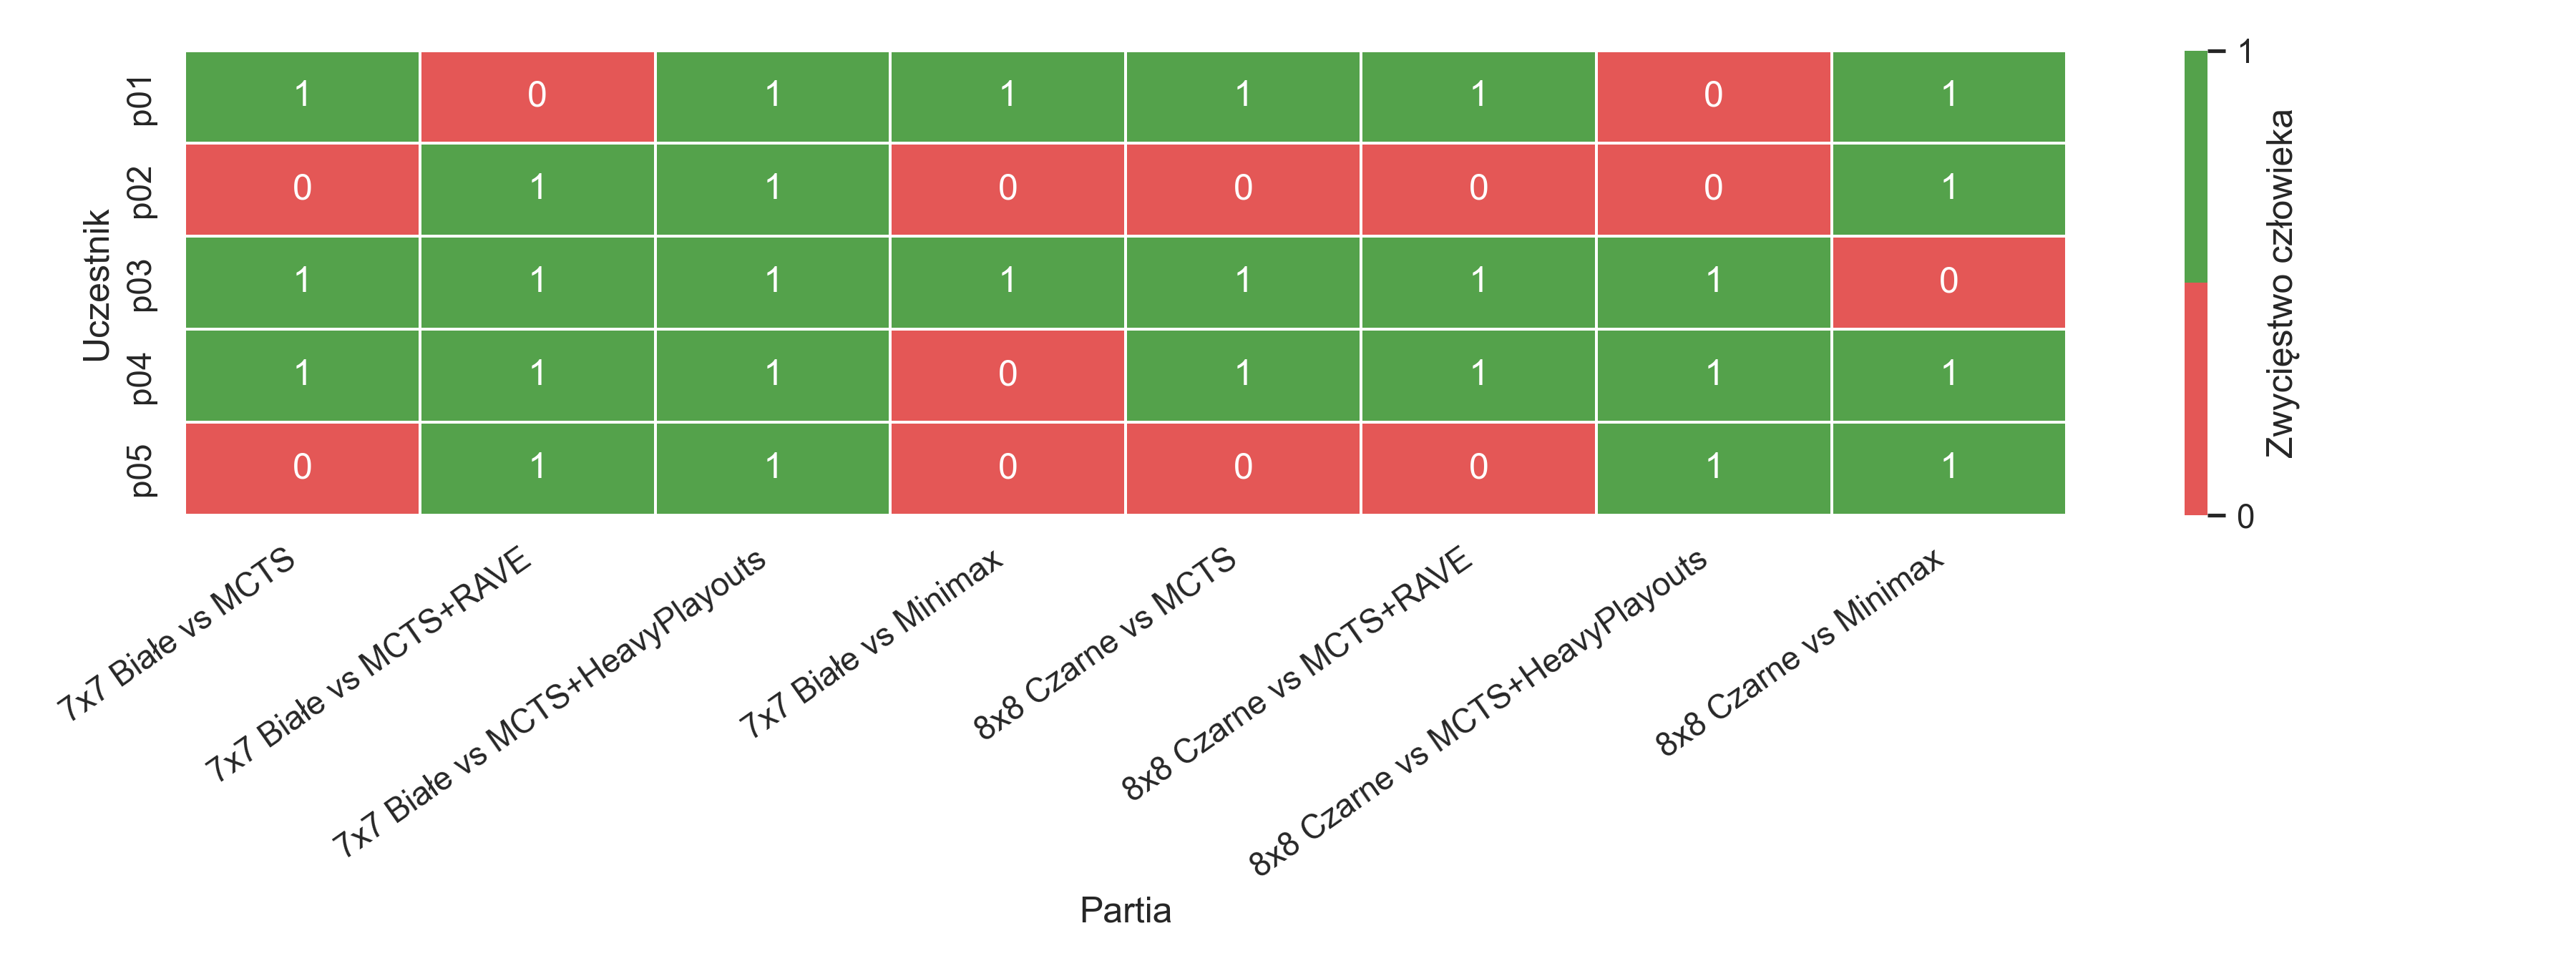
\includegraphics[width=\textwidth]{images/human_participant_outcomes.png}
    \caption{Macierz wyników poszczególnych uczestników. Wartość 1 oznacza zwycięstwo człowieka, natomiast 0 zwycięstwo agenta.}
    \label{fig:human-participant-outcomes}
\end{figure}

\noindent
Macierz wyników pokazuje dużą zmienność między uczestnikami. Mimo że każdy uczestnik został przeszkolony przed pierwszą rozgrywką, widoczna jest wyraźna dysproporcja pomiędzy badanymi. Jeden z testerów wygrał 7 z 8 partii, podczas gdy inny wygrał jedynie 3 z 8 partii. Gracze, którzy szybko zauważali podatność agentów MCTS na przepuszczanie wysuniętych pionów, byli w stanie regularnie wykorzystywać tę słabość. Z kolei gracze mniej konsekwentnie broniący wszystkich kolumn częściej dopuszczali do sytuacji, w której agent sam wymijał ich strukturę pionów.

\begin{table}[H]
    \centering
    \caption{Zestawienie wyników ludzi przeciwko poszczególnym wariantom AI.}
    \label{tab:human-summary}
    \renewcommand{\arraystretch}{1.2}
    \small
    \begin{tabularx}{\textwidth}{|p{4.0cm}|p{1.8cm}|p{1.8cm}|p{2.2cm}|X|}
        \hline
        \textbf{Przeciwnik} & \textbf{Wygrane ludzi} & \textbf{Wygrane AI} & \textbf{Skuteczność ludzi} & \textbf{Śr. długość partii} \\
        \hline
        MCTS & \hfill 6/10 & \hfill 4/10 & \hfill 60.0\% & \hfill 40.5 \\
        MCTS + RAVE & \hfill 7/10 & \hfill 3/10 & \hfill 70.0\% & \hfill 52.2 \\
        MCTS + Heavy Playouts & \hfill 8/10 & \hfill 2/10 & \hfill 80.0\% & \hfill 50.9 \\
        Minimax & \hfill 6/10 & \hfill 4/10 & \hfill 60.0\% & \hfill 56.1 \\
        \hline
    \end{tabularx}
\end{table}

\subsection{Długość partii i zachowanie materiału}

Oprócz samego wyniku przeanalizowano również liczbę wykonanych ruchów oraz liczbę pionów pozostających na planszy po zakończeniu partii. Metryki te pozwalają wnioskować, jak szybko przełamywana była linia przeciwnika.

\begin{figure}[H]
    \centering
    \begin{subfigure}[b]{0.49\textwidth}
        \centering
        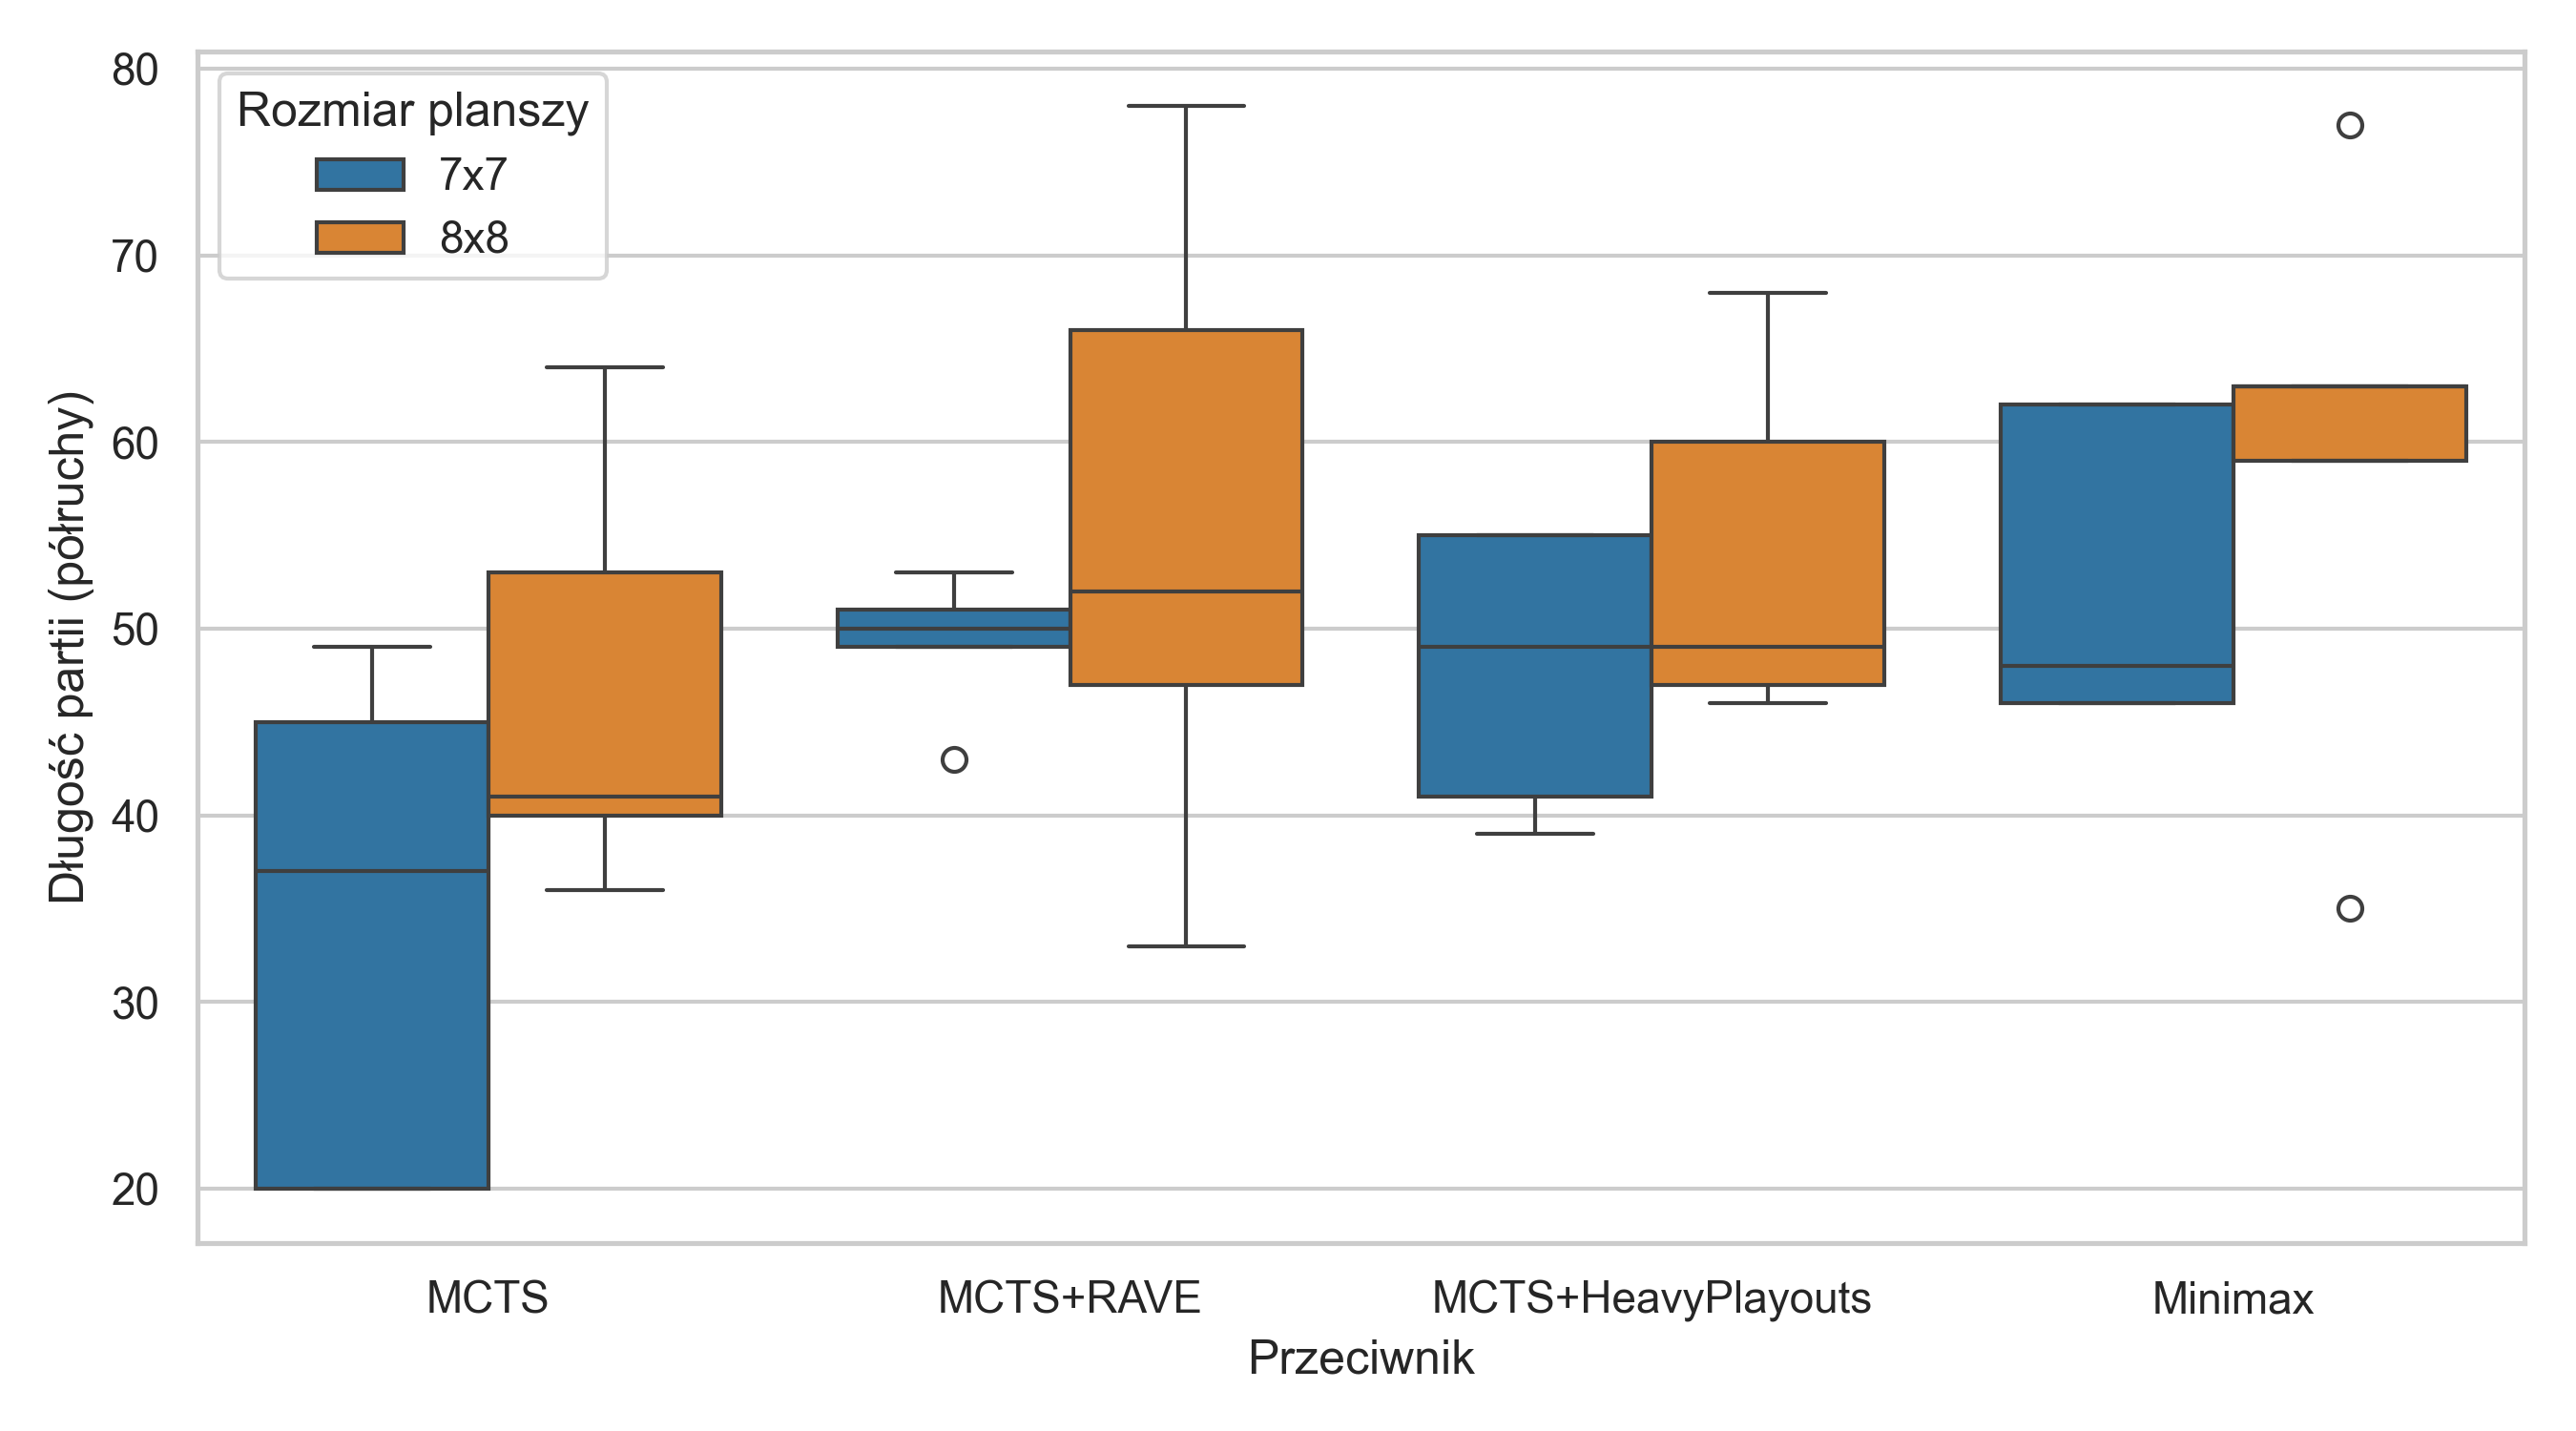
\includegraphics[width=\textwidth]{images/human_game_length_by_agent.png}
        \caption{Łączna długość partii}
        \label{fig:human-game-length}
    \end{subfigure}
    \hfill
    \begin{subfigure}[b]{0.49\textwidth}
        \centering
        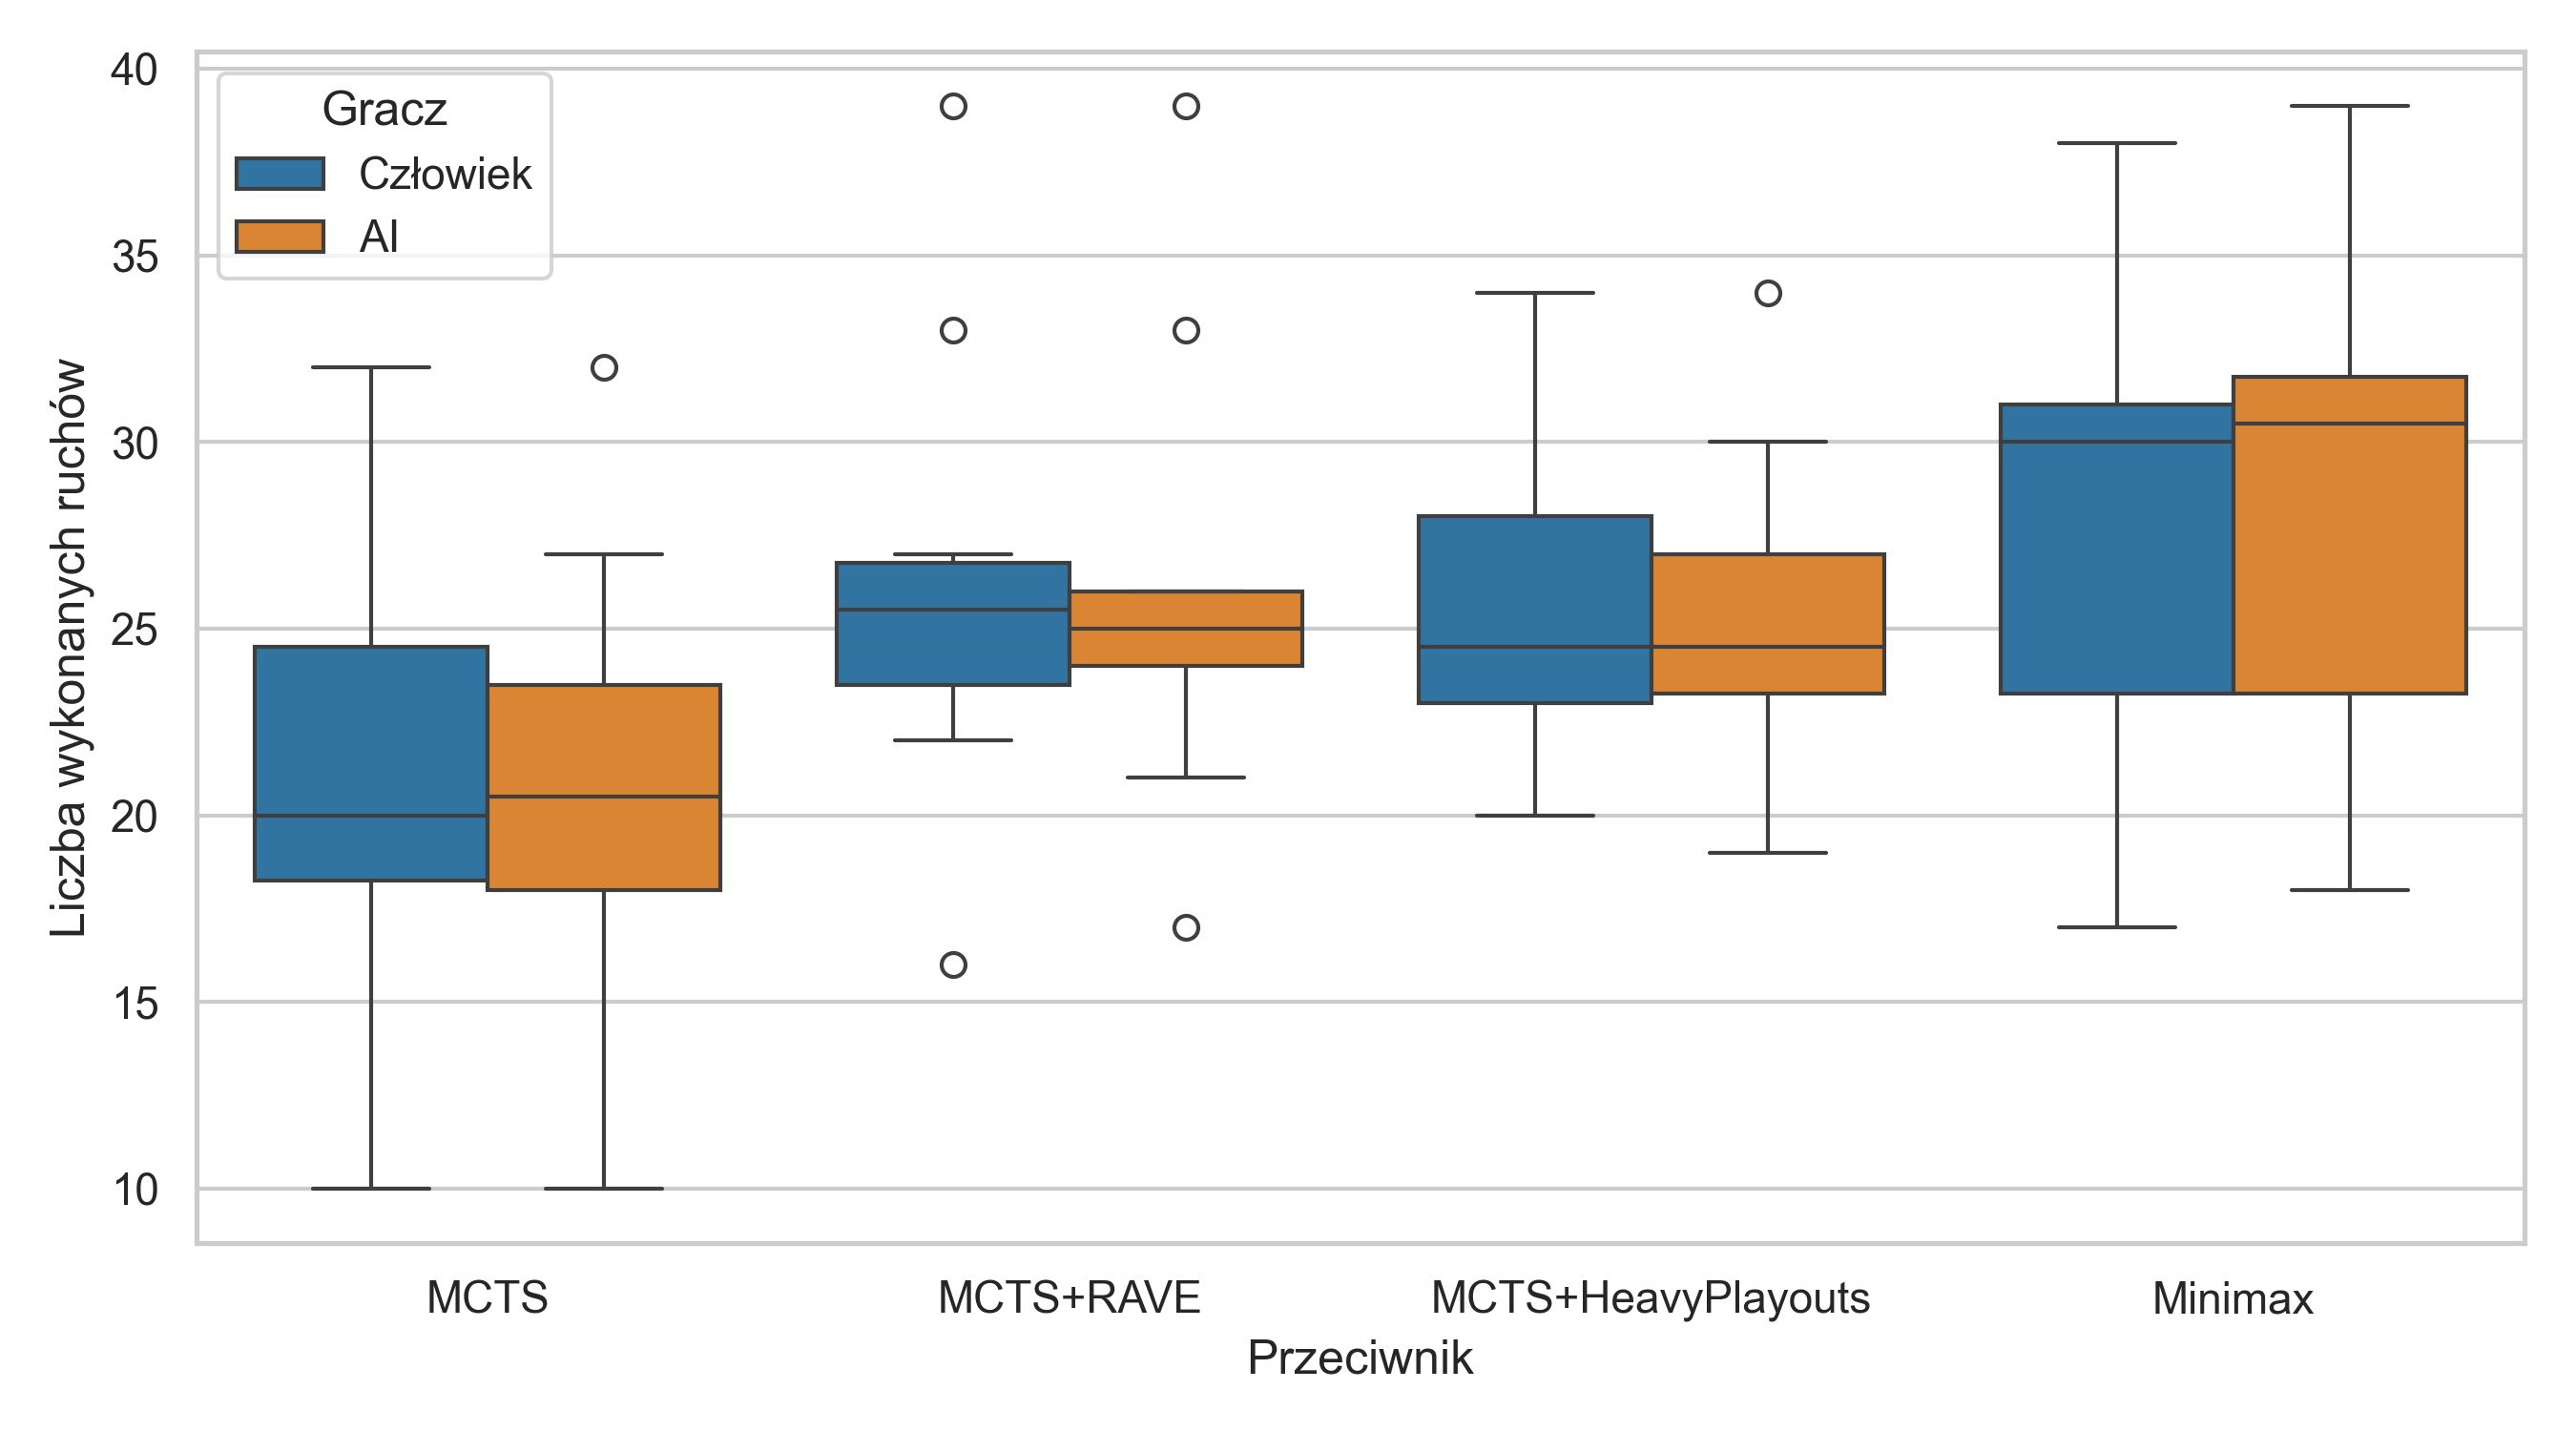
\includegraphics[width=\textwidth]{images/human_moves_by_agent.png}
        \caption{Liczba ruchów wykonanych przez strony}
        \label{fig:human-moves}
    \end{subfigure}
    \caption{Porównanie długości partii oraz liczby ruchów wykonanych przez człowieka i agenta.}
    \label{fig:human-length}
\end{figure}

\noindent
Najkrótsze partie występowały przeciwko klasycznemu MCTS, gdzie średnia długość wyniosła 40.5 półruchu. Partie przeciwko Minimaxowi były najdłuższe i trwały średnio 56.1 półruchu. Wynik ten jest zgodny z obserwacjami jakościowymi: Minimax często grał bardziej zwartą strukturą, przesuwał większą część linii pionów do przodu i rzadziej natychmiastowo odsłaniał pojedynczą kolumnę. W efekcie partia wymagała od człowieka dłuższego szukania przełamania lub obrony. Klasyczny wariant MCTS często bez widocznego uzasadnienia oddawał swoje piony w środkowych kolumnach. Następnie próbował zapełnić powstałą lukę pionami z bocznych stref planszy, co odsłaniało skrzydła i pozwalało badanym kończyć partie właśnie tymi kanałami.

W przypadku wariantów MCTS liczba ruchów człowieka i agenta była bardzo zbliżona, co wynika z naprzemiennego charakteru gry. Różnice można jednak zauważyć na Rysunku~\ref{fig:human-pieces}, który przedstawia liczbę pionów pozostających na planszy po zakończeniu partii.

\begin{figure}[H]
    \centering
    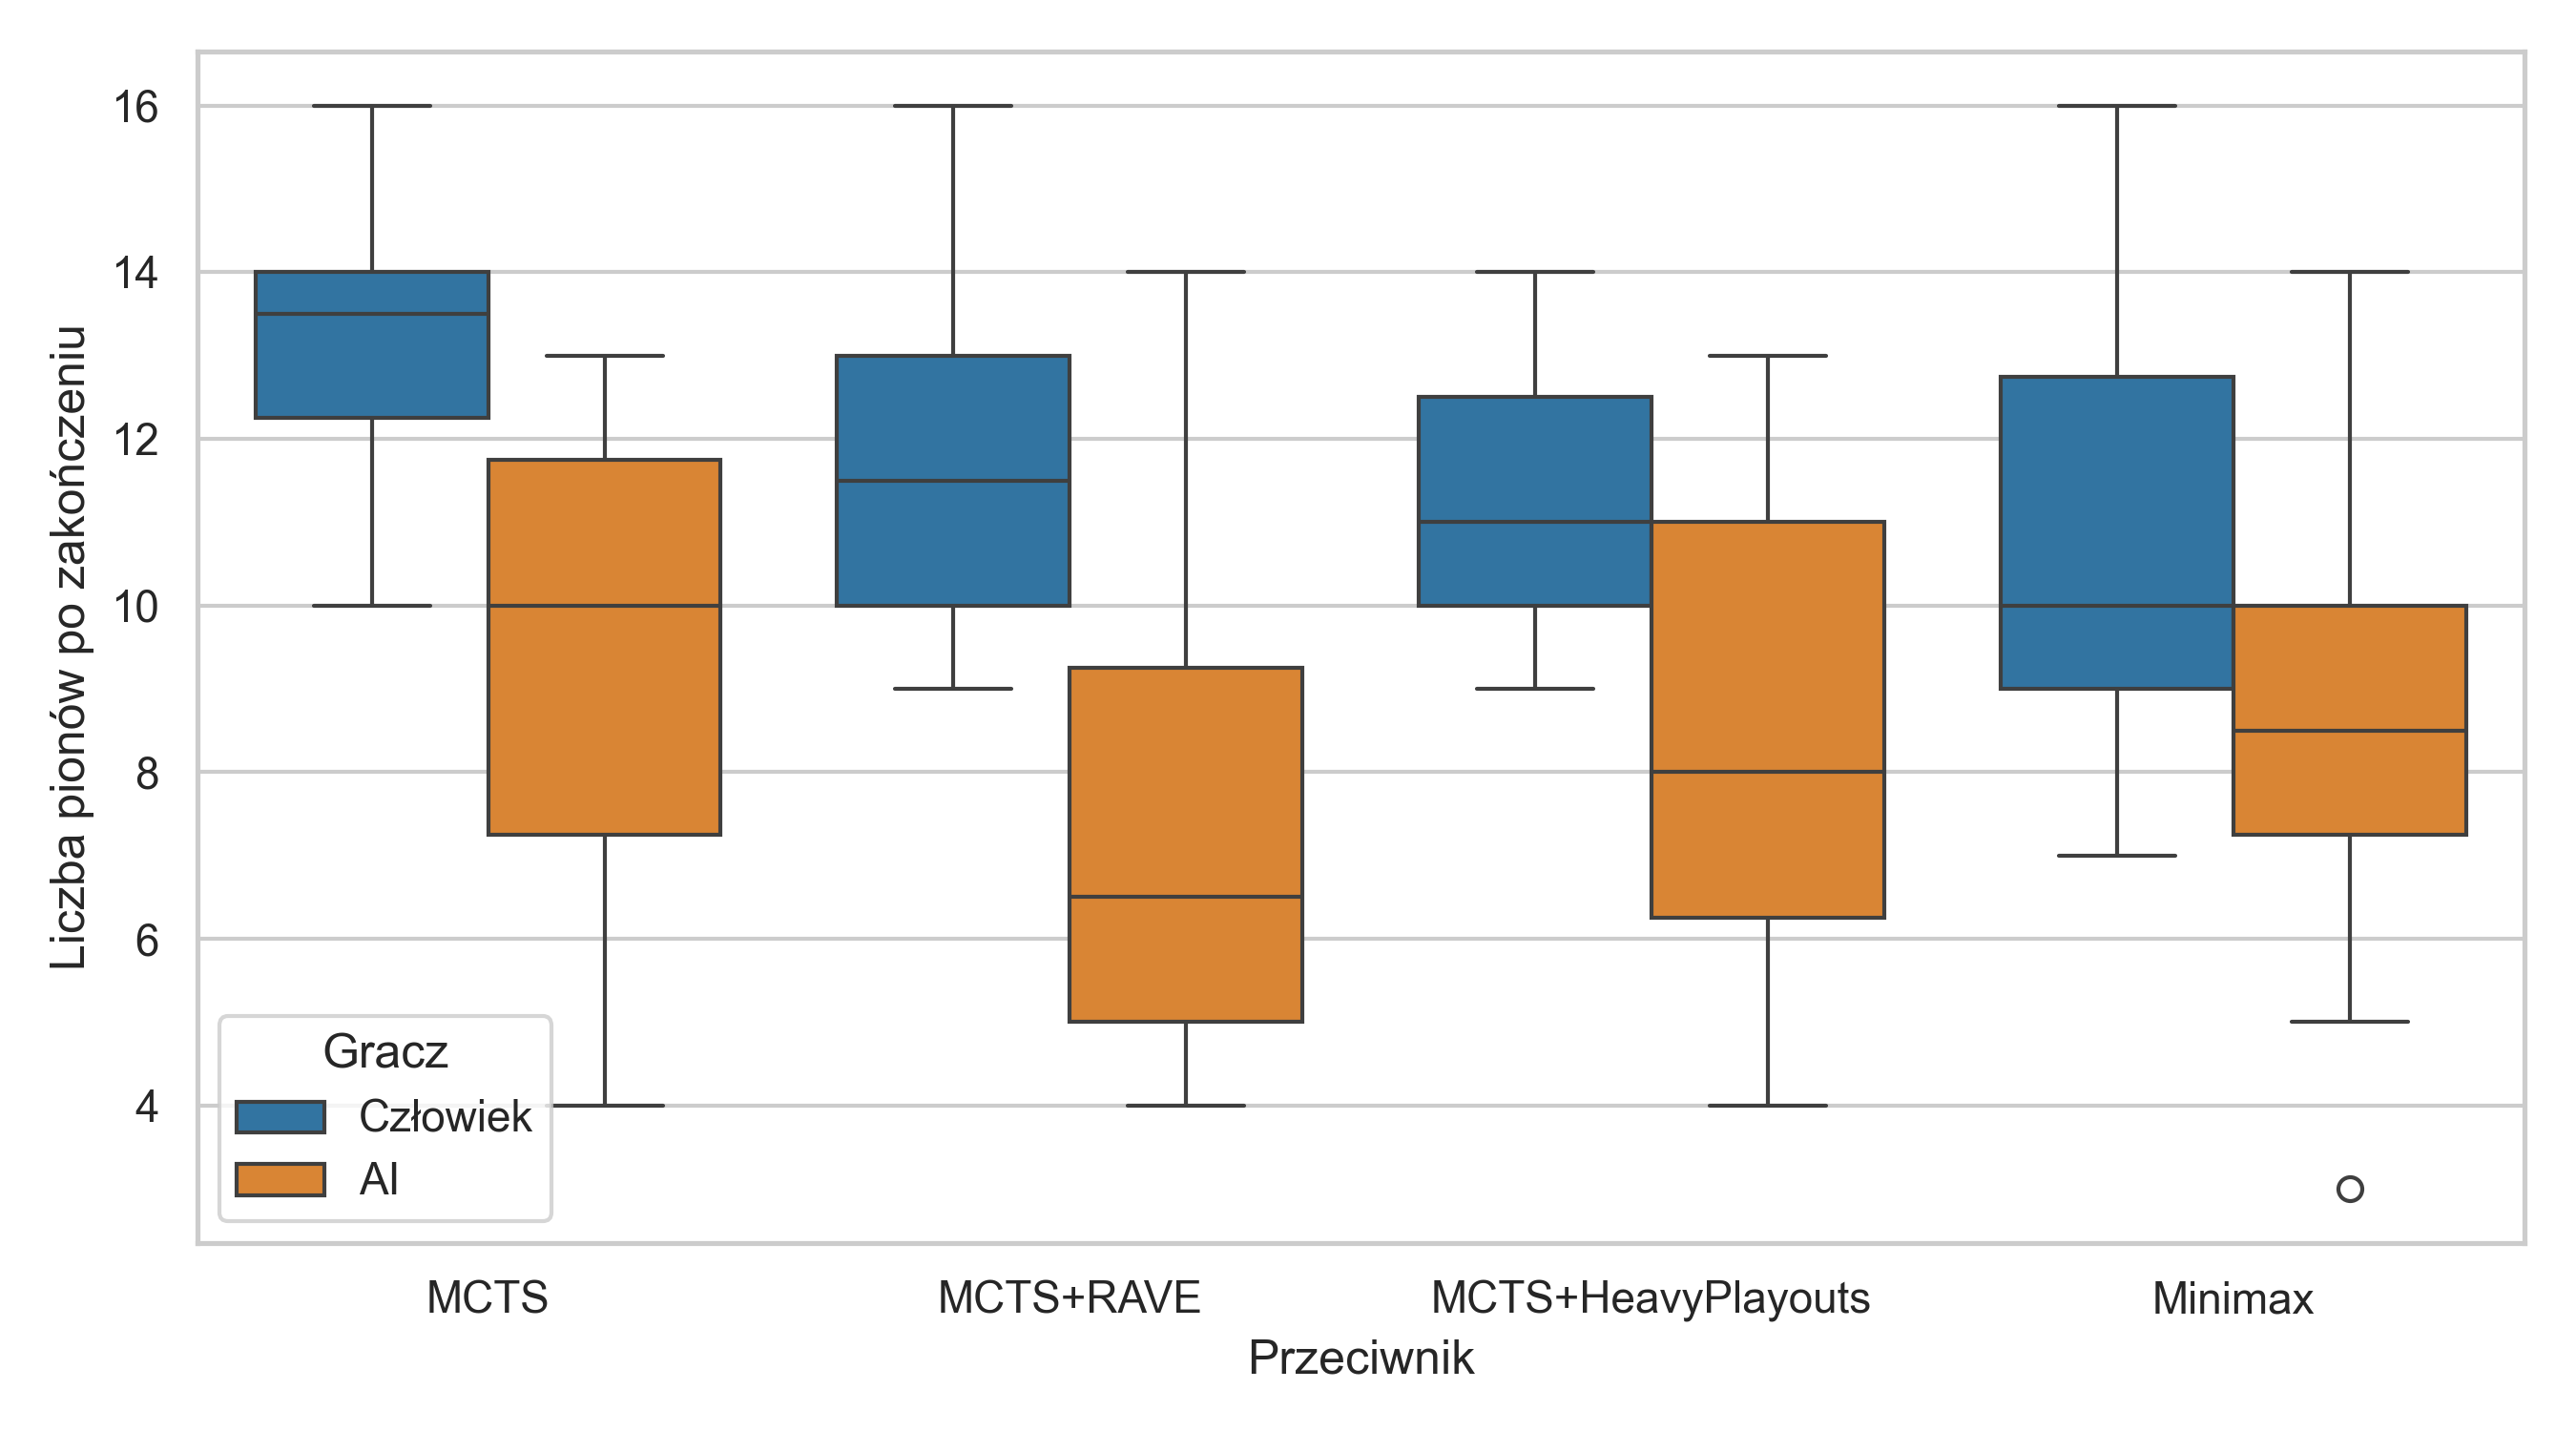
\includegraphics[width=0.85\textwidth]{images/human_pieces_remaining_by_agent.png}
    \caption{Liczba pionów człowieka i agenta pozostających na planszy po zakończeniu partii.}
    \label{fig:human-pieces}
\end{figure}

\noindent
We wszystkich wariantach końcowa przewaga materialna była po stronie ludzi. Średnio po partiach przeciwko MCTS człowiek zachowywał 13.2 pionu, a agent 9.3 pionu. Dla MCTS + RAVE wartości te wynosiły odpowiednio 11.9 oraz 7.4 pionu, dla MCTS + Heavy Playouts 11.3 oraz 8.2 pionu, natomiast dla Minimaxa 10.8 oraz 8.4 pionu. Przyczyną takiej dysproporcji może być to, że w pozycjach przegranych agenci poświęcali piony, starając się opóźnić porażkę. Badani, mimo że często mogli już bezpośrednio wygrać partię, zbijali podstawiane piony, budując dodatkową przewagę materialną. Dysproporcja ta sugeruje również, że zwycięstwa ludzi nie były wyłącznie efektem pojedynczego szybkiego przebicia lub sprytnego ruchu, lecz często wiązały się ze stopniowym budowaniem przewagi strukturalnej i materialnej.

\subsection{Ocena ankietowa i obserwacje jakościowe}

Uczestnicy oceniali trudność oraz naturalność ruchów przeciwników w skali od 1 do 5. Zestawienie średnich ocen przedstawiono na Rysunku~\ref{fig:human-survey}. Najwyżej ocenionym wariantem w obu kategoriach był Minimax. Średnia ocena trudności wyniosła dla niego 3.7, a naturalności strategii 4.1. Klasyczny MCTS uzyskał średnią trudność 3.1 i naturalność 2.9, MCTS + RAVE odpowiednio 2.8 i 2.8, natomiast MCTS + Heavy Playouts 2.8 i 3.3.

\begin{figure}[H]
    \centering
    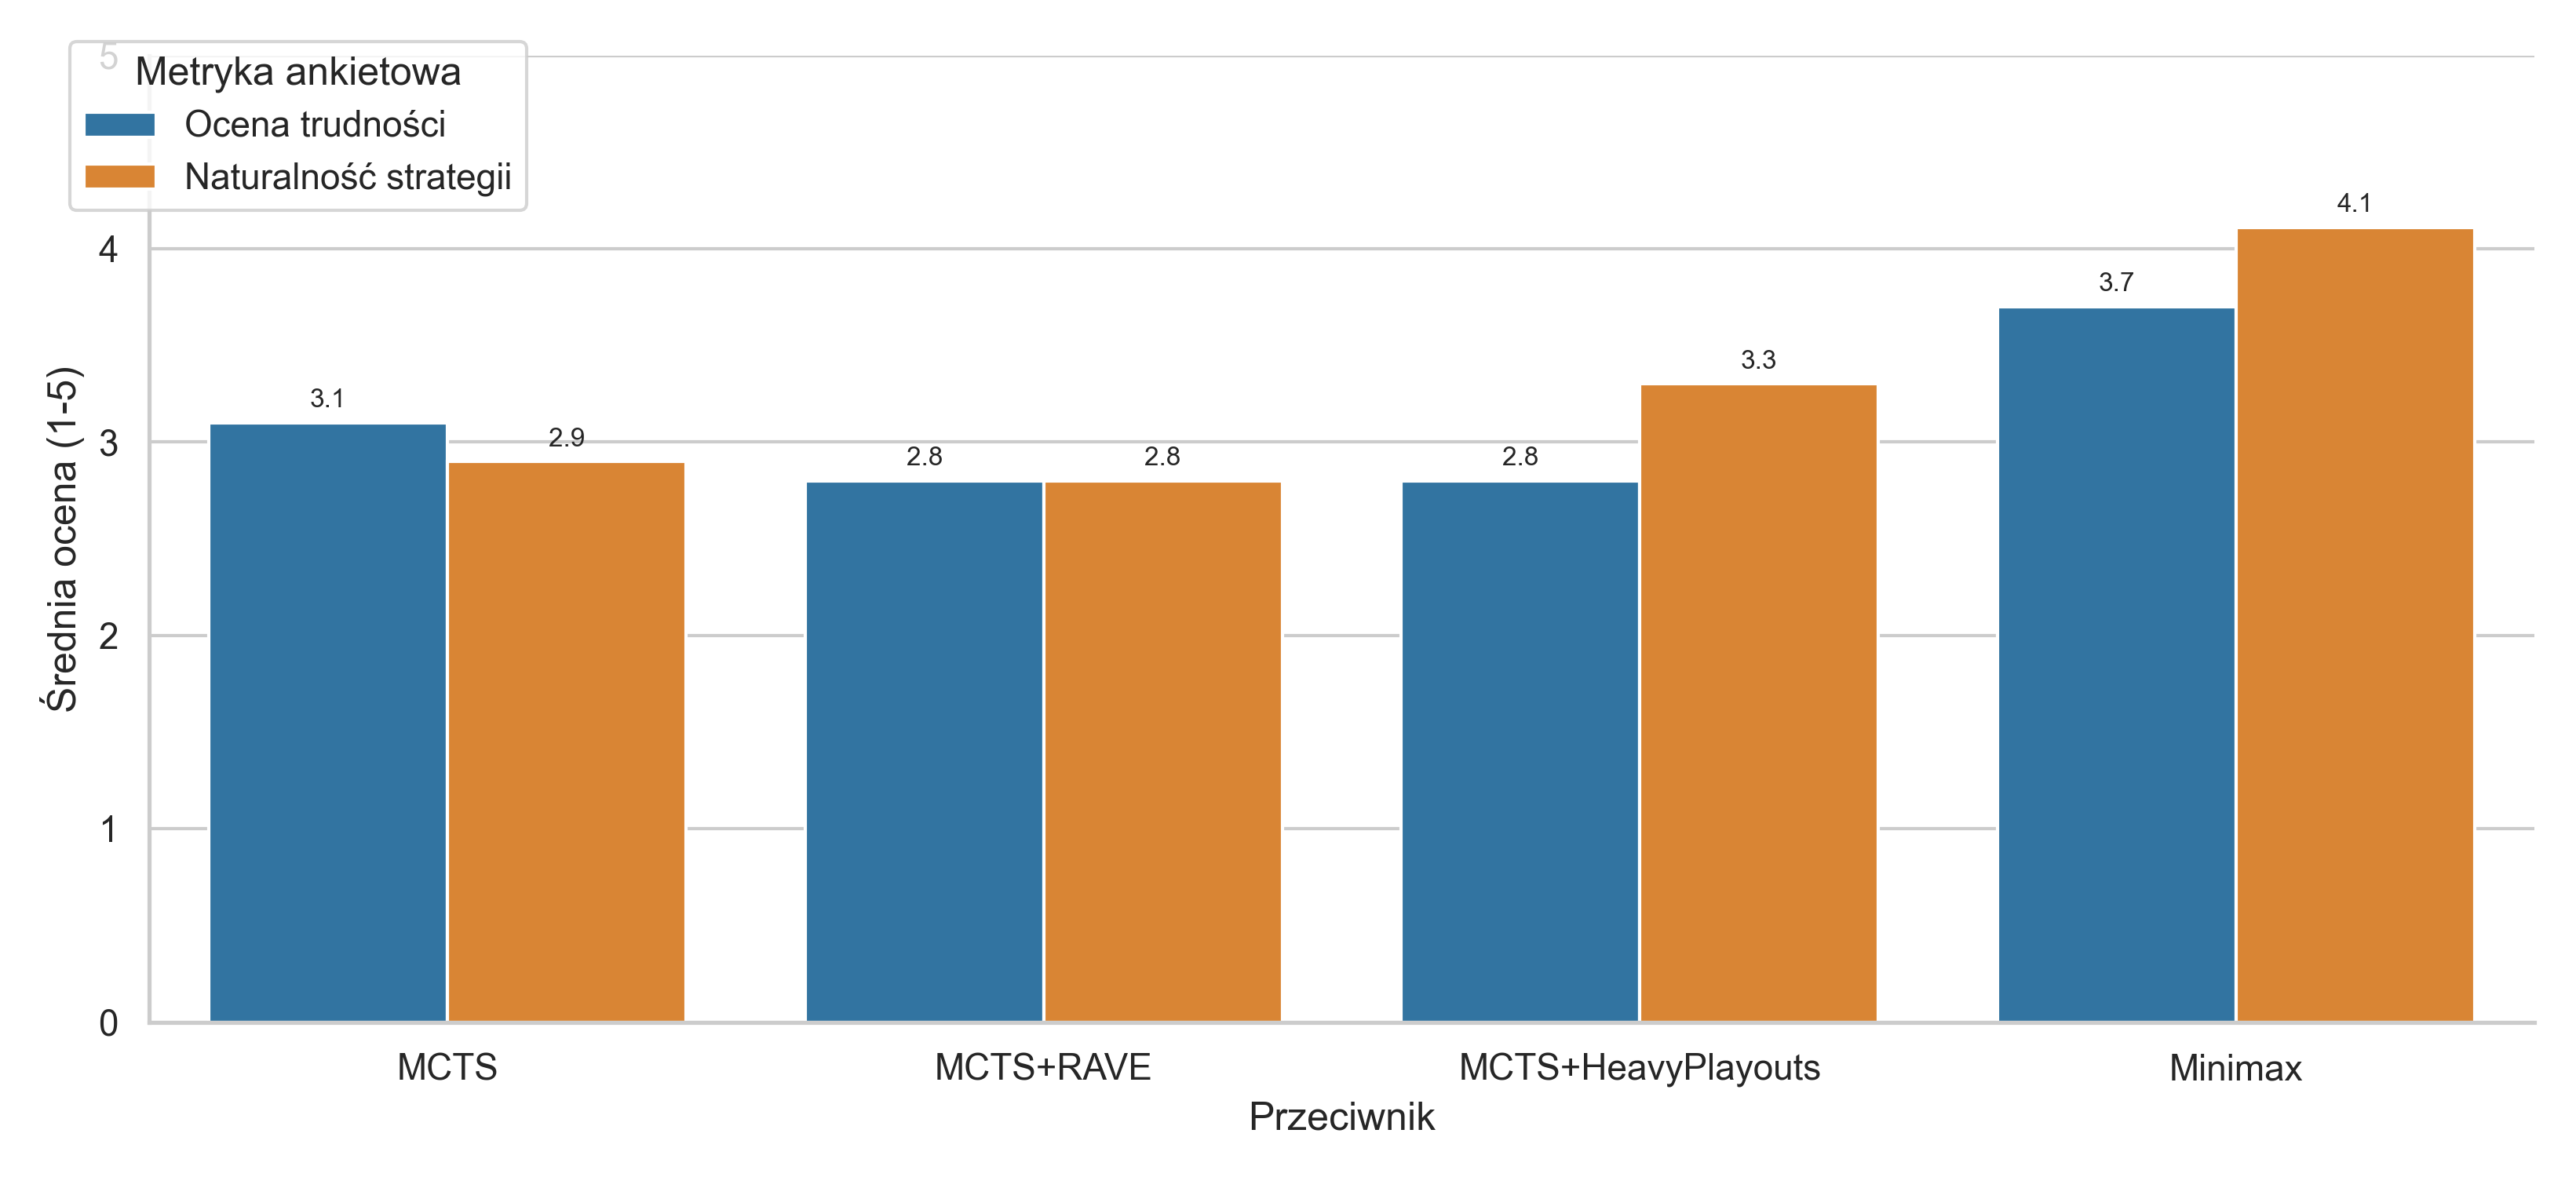
\includegraphics[width=0.82\textwidth]{images/human_survey_ratings_by_agent.png}
    \caption{Średnie oceny ankietowe przeciwników AI w skali od 1 do 5.}
    \label{fig:human-survey}
\end{figure}

\noindent
Oceny ankietowe są spójne z feedbackiem testerów oraz z obserwacjami prowadzonymi podczas rozgrywek. Minimax był odbierany jako przeciwnik najbardziej agresywny i najbardziej planowy. Testerzy zwracali uwagę, że często przesuwał całą linię pionów w sposób symetryczny, przez co wymuszał analizę kilku możliwych przełamań jednocześnie. Na planszy $8 \times 8$ przeciętny badany miał trudność z konsekwentnym sprawdzaniem wszystkich ruchów do przodu, podczas gdy Minimax systematycznie przeszukiwał takie możliwości. 

Warianty MCTS były oceniane bardziej ambiwalentnie. Testerzy zauważali, że potrafiły dobrze bronić zastawione pułapki oraz reagować na przenoszenie pionów na jedną stronę planszy. Wielokrotnie udawało im się ominąć strukturę obronną zbudowaną przez badanego. Często pojawiały się też podobne schematy gry, na przykład ustawianie dwóch pionów jeden za drugim w jednej kolumnie. Dzięki takiemu ustawieniu bicie lub łatwe ominięcie struktury staje się trudniejsze. Z drugiej strony klasyczny MCTS oraz MCTS + RAVE miewały tendencję do zbyt odważnego wypychania najbardziej wysuniętego pionu, co w praktyce prowadziło do oddawania materiału. Według autorów prawdopodobną przyczyną jest losowy charakter fazy \textit{playout}: w symulacjach takie zagranie nie zawsze kończy się natychmiastową karą, ponieważ zbicie pionu jest tylko jedną z wielu losowych możliwości, a czasem wysunięty pion może przypadkowo doprowadzić do zwycięstwa, zaburzając statystyki drzewa.

Ostatnią obserwacją zgłoszoną w ankietach było to, że gdy agent znajdował się w sytuacji trudnej do obrony, często zaczynał wykonywać ruchy poświęcające materiał w celu opóźnienia porażki. Z perspektywy człowieka wyglądało to czasem jak desperackie oddawanie pionów, ale jest to naturalna konsekwencja funkcji celu agenta. Wpływ tego zachowania na liczbę pionów pozostałych na planszy po zakończeniu rozgrywki został opisany wcześniej.

\subsection{Wnioski końcowe}

Testy z udziałem ludzi pokazały, że skuteczność agentów w rozgrywkach automatycznych nie przekłada się bezpośrednio na odbiór ich siły przez badanych. Pomimo tego, że Minimax osiągał miażdząco najlepsze wyniki w poprzednich eksperymentach, a gracze z najlepszym współczynnikiem zwycięstw przegrywali pojedyncze partie tylko z nim, całościowo nie osiągnął on ewidentnie najlepszego wyniku procentowego przeciwko ludziom. Wynika to z jego deterministycznego, taktycznego charakteru gry: nawet jeśli popełniał błędy wynikające z ograniczonej funkcji heurystycznej, jego ruchy częściej sprawiały wrażenie elementów spójnego planu. Był to jednak wariant, który nie wybaczał błędów i jeśli znajdował sekwencję ruchów prowadzącą do zwycięstwa, konsekwentnie ją realizował.

Warianty MCTS, zwłaszcza bez Heavy Playouts, częściej ujawniały zachowania trudne do uznania za ludzkie: nadmierne wysuwanie pojedynczych pionów, lokalne oddawanie materiału oraz brak wyraźnej symetrii w strukturze. Strategie te nie były jednak całkowicie losowe, co potwierdzają spostrzeżenia badanych. Badanie z ludźmi wskazuje, że stabilność gry, reakcja na błędy przeciwnika oraz subiektywne wrażenie planowości nie muszą bezpośrednio pokrywać się z końcowym wynikiem partii. Ostatecznie w grze liczy się zwycięstwo, ale przy ocenie agenta warto pamiętać również o tym, jak jego styl jest odbierany przez człowieka. Nie można też zapominać, że próba była bardzo mała, a różnice w odsetkach zwycięstw między wariantami są ograniczone.

\newpage
\section{Podsumowanie}

Celem niniejszego projektu była implementacja, optymalizacja oraz ewaluacja algorytmu Monte-Carlo Tree Search (MCTS) wraz z jego modyfikacjami w środowisku deterministycznej gry planszowej Breakthrough. W tym celu stworzono w pełni funkcjonalny system w języku Rust, obejmujący silnik obliczeniowy do porównywania różnych wariantów algorytmu w zautomatyzowanych turniejach self-play oraz graficzny interfejs użytkownika przeznaczony do testów z udziałem ludzi.

Przeprowadzone eksperymenty pozwoliły zweryfikować cztery wcześniej postawione hipotezy oraz sformułować wnioski dotyczące przeszukiwania przestrzeni stanów w grze Breakthrough. Weryfikacja hipotezy H1 pokazała, że samo zastosowanie heurystyki RAVE (AMAF) nie przyniosło oczekiwanej poprawy jakości gry. Ze względu na taktyczny charakter Breakthrough kolejność ruchów oraz tempo dojścia do linii końcowej mają duże znaczenie, dlatego kluczowe założenie RAVE o względnej niezależności wartości ruchu od momentu jego wykonania okazało się w tym przypadku zbyt silne.

Odmienne rezultaty przyniosła weryfikacja hipotezy H2. Wprowadzenie wiedzy domenowej do fazy symulacji wyraźnie podniosło skuteczność agenta w starciu z klasycznym wariantem. Poprawa ta wystąpiła mimo istotnego narzutu obliczeniowego powodowanego przez Heavy Playouts. Wskazuje to, że podniesienie jakości pojedynczej symulacji może kompensować straty wynikające ze zwiększonego czasu obliczeń i mniejszego rozmiaru generowanego drzewa gry.

Starcia wariantów probabilistycznych z deterministycznym algorytmem Minimax w ramach H3 ukazały słabość metod statystycznych przy średnich horyzontach planowania oponenta. Jednocześnie ponownie widoczna była przewaga MCTS + Heavy Playouts nad klasycznym wariantem oraz RAVE, ponieważ był to jedyny wariant MCTS, który nie odstawał wyraźnie od Minimaxa. Badania nad geometrią planszy w ramach H4 pokazały natomiast, że wydłużenie dystansu między graczami skutecznie ogranicza asymetrię szans wynikającą z przewagi pierwszego ruchu białych.

Istotnych obserwacji dostarczyły również testy z udziałem ludzkich graczy. Pokazały one różnicę między skutecznością agenta w starciach z innymi wariantami AI a jego skutecznością w grze przeciwko człowiekowi. Paradoksalnie, agent MCTS + Heavy Playouts, który był zdecydowanym zwycięzcą turnieju różnych wariantów MCTS, okazał się najłatwiejszy do pokonania przez ludzi. Najtrudniejszymi przeciwnikami były natomiast Minimax, tworzący spójne struktury defensywne i logiczne sekwencje bić, oraz klasyczny MCTS. Może to sugerować, że heurystyki optymalizowane pod kątem ulepszania symulacji generują luki taktyczne, które ludzka intuicja potrafi stosunkowo szybko zidentyfikować i wykorzystać.

Podsumowując, zastosowanie metod opartych na Monte-Carlo Tree Search w grze Breakthrough stanowi skuteczne rozwiązanie, choć jego efektywność silnie zależy od sposobu wykorzystania wiedzy domenowej. Kolejnym kierunkiem badań mogłoby być łączenie kilku modyfikacji algorytmu lub jego poszczególnych faz, w szczególności połączenie Heavy Playouts z RAVE oraz wykorzystanie zrównoleglenia obliczeń. Interesującym obszarem dalszych analiz byłaby także modyfikacja funkcji heurystycznej tak, aby lepiej odzwierciedlała taktyki wykorzystywane przez silnych graczy. Najlepsze wyniki w eksperymentach automatycznych zapewniał wariant Minimax, jednak stworzenie agenta, który nie tylko optymalizuje współczynnik zwycięstw, lecz także prezentuje styl gry wymagający od człowieka naturalnej i elastycznej odpowiedzi, pozostaje otwartym wyzwaniem.

%----------------------------------------------------------------------
\newpage
\begin{thebibliography}{9}

\bibitem{rust-install}
\emph{The Rust Programming Language -- Installation}, \url{https://doc.rust-lang.org/book/ch01-01-installation.html\#installation} (dostęp 28.01.2026r.).

\bibitem{rustc-man}
\emph{What is rustc?}, \url{https://doc.rust-lang.org/stable/rustc/index.html\#what-is-rustc} (dostęp 28.01.2026r.).

\bibitem{cargo-book}
\emph{The Cargo Book -- Installation}, \url{https://cargo-book.irust.net/en-us/getting-started/installation.html} (dostęp 28.01.2026r.)

\end{thebibliography}

\end{document}
